%%%%%%%%%%%%%%%%%%%%%%%%
% Sample use of the infthesis class to prepare an MSc thesis.
% This can be used as a template to produce your own thesis.
% Date: June 2019
%
%
% The first line specifies style options for taught MSc.
% You should add a final option specifying your degree.
% *Do not* change or add any other options.
%
% So, pick one of the following:
% \documentclass[msc,deptreport,adi]{infthesis}     % Adv Design Inf
% \documentclass[msc,deptreport,ai]{infthesis}      % AI
% \documentclass[msc,deptreport,cogsci]{infthesis}  % Cognitive Sci
% \documentclass[msc,deptreport,cs]{infthesis}      % Computer Sci
% \documentclass[msc,deptreport,cyber]{infthesis}   % Cyber Sec
% \documentclass[msc,deptreport,datasci]{infthesis} % Data Sci
% \documentclass[msc,deptreport,di]{infthesis}      % Design Inf
% \documentclass[msc,deptreport,inf]{infthesis}     % Informatics
%%%%%%%%%%%%%%%%%%%%%%%%

\documentclass[mphil,deptreport,ianc]{infthesis} % Do not change except to add your degree (see above).
\usepackage[final]{pdfpages}
\usepackage{siunitx}
\usepackage{hyperref}
\hypersetup{
    colorlinks=true,
    linkcolor=black,
    filecolor=gray,
    urlcolor=blue,
    pdftitle={Spiking neural network model inference},
    pdfpagemode=FullScreen,
    }
\usepackage[section]{placeins}
\usepackage{amsmath}% \usepackage[printonlyused,withpage]{acronym}
\usepackage[withpage]{acronym}

\begin{document}
\begin{preliminary}


\title{Spiking neural network model construction, inference, analysis and applications}

\author{William Peer Berg}

    
\abstract{
    Computational models have long been used as hypotheses to illuminate and unravel aspects of neural functioning, with seminal works including models such as the Hodgkin-Huxley model,
    which also exemplifies that model hypotheses may be tested with in vivo or vitro experiments.
    However, designing high-dimensional biologically realistic spiking models can be an arduous endeavour, and may require a large amount of resources in hand-engineering.
    Automating this arduous process could potentially greatly accelerate computational research within neuroscience.
    Therefore, statistical approaches have been used to try and aid in such modelling, with the current state-of-the-art being based on approximate Bayesian computation.
    However, this approach does not scale well with growing model size and complexity, i.e. both the number of neurons and the number of parameters.
    In the current data driven era, where deep learning is the prevalent state-of-the-art within machine learning, we investigate whether its key ingredient; gradient based optimisation (GBO) may be leveraged for spiking neural network (SNN) model inference.
    To this end we implement a modular gradient based optimisation framework on top of PyTorch, a modern ML Python library, and test to what extent GBO may be used for SNN inference, particularly because this approach scales well with network size.
    GBO is tested for a rate based loss metric, the van Rossum distance which also emphasises the timing of spiking, for the Bernoulli or Poisson negative log-likelihood for probabilistic stochastic models, over different classes of SNNs, including generalised versions of leaky integrate-and-fire, non-leaky integrate-and-fire, and probabilistic general integrate-and-fire spiking models, with extensions to subthreshold synaptic current models as the readout signal used during optimisation instead of a surrogate over the membrane potential, which greatly increases optimisation performance.
    The results show that due to the temporal state-dependence of the membrane potentials and thus spikes in SNNs, the van Rossum distance metric and emphasis on the precise timing of spiking may obscure the gradient signal.
    As for the spike trains themselves produced by the models, we test whether higher-order statistics are captured to a greater extent in the SNNs irrespective of the loss variability, and compare model fits to generalised linear models as a baseline model.
    When factorising the spike trains by using non-negative matrix factorisation (NMF), the resulting ensembles reveal similar functional ensembles for the synthetic data - however, the SNNs capture the functional NMF ensembles to a greater extent, reflected in a higher NMF module similarity.
    When testing whether this was due to inductive bias by SNN model definition by also fitting to biological data, we found that indeed the similarity was greater for the SNN models than for GLMs, suggesting that GBO may be leveraged to some extent for SNN inference with regards to capturing higher-order spike train statistics.
    Further, the parameter landscapes formed by the rate-based metric contains no global saddle point, and at best a frontier as the global minima.
    These observations and results are reflected in the inferred parameters when compared to the ground-truth models for the synthetically generated data, where the inferred SNN likely retrieved a different parameter configuration, while yet capturing the higher-order spike statistics, or solving the task at hand.
    When introducing a lower-dimensional intput-output task and using a readout of a continuous subthreshold synapse current model as the output, we were able to show that optimisation convergence was robust, and that the tasks were solved with low error - albeit yet with completely different final SNN parameter values.
    This emphasises the point that the biological brain may elegantly solve different tasks with completely different configurations, as is the case in every individual, and may suggest that we should not seek to retrieve some target parameter values, as much as higher-order spike statistics.
}


\maketitle

\section*{Lay summary}

Computational models are a highly useful tool, employed in nearly all domains of science and engineering. A model is in itself a hypothesis of a system that we’re studying - whether in biology, physics, or psychology.
Some of these models, particularly within computational neuroscience, are more complex than others. As such, they may better and in a more detailed way describe what is going on in the biological system that we’re modeling - by in fact being a closer match to the system, such as for instance a collection of neurons from which we have recorded signals using probes.
A fundamental issue with these models is however that we do not currently have a satisfactory way of automatically inferring and attaining them, i.e. there is not algorithm or procedure that allows us to infer such model, no matter how much data we may have.
Therefore, researchers often spend a great deal of time and resources in hand-engineering such models, which also typically requires expert knowledge.
As such, a central challenge in computational neuroscience, which could greatly aid in modeling research, is how one might go about inferring more biologically realistic models.
With the recent widespread success of the algorithmics applied in deep learning, which has given rise to successful applications and better models in a myriad of different disciplines, we investigate whether we may combine the technique employed within deep learning, namely gradient based optimisation, with inference of a more biologically realistic class of neural networks; spiking neural networks.
These networks are more realistic in that each neuron models a membrane potential, and potentially more parameters that represent biological properties.
We look at what has been done up until now for this model type, including a range of different such spiking models, and implement inference using the aforementioned gradient based optimisation methodology in a modern machine learning library called PyTorch.
This lets us test to what extent the model reproduces and behaves like the data that we feed it during training/inference, as well as whether the model itself looks similar to what we would expect when comparing to either another model that has generated data, or to some biological properties.
Further, we can look at whether the neurons spike in similar patterns and ensembles on a network-level.
It turns out that we may find models that behave similarly on a network-level, but not at all at a single-neuron level.
This may be expected if one considers that there are many different ways in which a network may capture similar patterns, potentially representing the same feature, or learning to perform some task.
% We begin by revisiting the state-of-the-art within the domain of spiking neural network models (SNNs), and then define a number of different SNNs. 
% We then describe how we may perform gradient based optimisation for SNNs, and how we may evaluate the inferred models, and describe how we have implemented this in a modern machine learning library in Python, called PyTorch.
% We test different ways of performing the optimisation, by guiding it differently with different functions defining the signal that we’re using for optimisation - called loss metrics, and adopt different works that introduce different model types, loss metrics, as well as data and model tasks.
% Overall, we find significant limitations to the current statistical approaches, particularly for when the SNNs increase in size or complexity. However, these might be overcome by using gradient based optimisation (GBO). In our experiments pertaining to GBO, we find that the exact model parameters vary greatly - but that the inferred model configuration yet capture the data, and optionally perform the task at hand well.
This may suggest that like in the biological brain, there is a myriad of possible solutions, and the precise configuration may not matter as much as commonly suggested. Arguably the precise wiring and neural ‘configuration’ varies greatly between individuals - what is crucial is that we functionally arrive at solving the task at hand well.
Furthermore, when we introduced a synapse (the cell that connects different neurons, and relays electric signals between them) model that varies continuously with the neurons’ excitation, as well as presented the model with a simpler training signal, both training and task performance were excellent. This might suggest a role in the slower waves observed in biological brain waves in learning, which also contains a parallel to the sleep research literature in that sleep is thought to also facilitate learning, and that we have this synchronous slow-wave mode of brain-wide activity during sleep.

\clearpage

\section*{Acknowledgements}

I would like to thank my supervisory team for offering their advice throughout my research.
I would also like to thank members of my lab group whom offered invaluable support and advice on everything from my project work to mastering stress and finding a flat in Edinburgh.
I also sincerely appreciated input relating to mathematics and philosophy from two special friends in Ediburgh whom are outside of my lab group.
I would also like to thank friends and family at home, whose support was important to me throughout my research.
Lastly, I would like to sincerely thank the head of our collaborative lab at the University of Strathclyde whom gave us access to in vivo data from the brainstem that was analysed with regards to sleep regulation. It was truly inspiring and exciting to be able to see their experimental lab from early on in my project work.

\clearpage
\section*{Declaration}

I declare that the thesis has been composed by myself and that the work has not been submitted for any other degree or professional qualification. I confirm that the work submitted is my own, except where otherwise stated.
% I have presented the included posters at the conferences UK Neural computation 2019, and the FENS forum 2020 (as indicated on the poster), and the included report was submitted to a conference (the International Conference on Machine Learning (ICML) 2021).
My contribution and that of collaborations have been referenced explicitly both in the text, and the collaborations are indicated below. I confirm that appropriate credit has been given within this thesis where reference has been made to the work of others.

Part of the work presented in Chapter \ref{chpt:sleep}, namely that in section \ref{subsect:bio_data} was previously published in the referenced paper: Tsunematsu, T., Patel, A. A., Onken, A., \& Sakata, S. (2019). State-dependent pontine ensemble dynamics and interactions with cortex across sleep states. BioRxiv, 752683. \href{https://doi.org/10.1101/752683}{DOI} \cite{Tsunematsu2019}, 
in which my principal supervisor is a co-author.
I did not contribute to this publication, but was granted access to the data used in the publication after its submission.
The data access was granted via the collaboration setup by my principal supervisor Arno Onken with the experimental lab led by Shuzo Sakata at the University of Strathclyde in Glasgow, Scotland.
I replicated some of the findings of the original study before proceeding to employ the data in the unrelated gradient based optimisation work presented in this thesis, and have stated that I have replicated findings where this is the case. 


% Nina.
% Matthias.
% Shuzo.
% Luke.
% Patricia.
% Etienne.

\tableofcontents

\clearpage
\section*{List of Acronyms}
\begin{acronym}
 \acro{GBO}{Gradient based optimisation}
 \acro{SNN}{Spiking neural network}
 \acro{NMF}{Non-negative matrix factorisation}
 \acro{ML}{Machine learning}
 \acro{RNN}{Recurrent neural network}
 \acro{DNN}{Deep neural network}
 \acro{LIF}{Leaky integrate-and-fire}
 \acro{GLIF}{Generalised leaky integrate-and-fire}
 \acro{NLIF}{Non-leaky integrate-and-fire}
 \acro{SGIF}{Stochastic general integrate-and-fire}
 \acro{GLM}{Generalised linear model}
 \acro{ABC}{Approximate bayesian computation}
 \acro{SBI}{Simulation-based inference}
 \acro{ODE}{Ordinary differential equation}
 \acro{BP}{Backpropagation}
 \acro{BPTT}{Backpropagation through time}
 \acro{GD}{Gradient descent}
 \acro{HH}{Hodgkin-Huxley}
 \acro{XOR}{Exclusive-or}
 \acro{GRU}{Gated recurrent unit}
 \acro{LDA}{Linear discriminant analysis}
 \acro{PDF}{Probability density function}
 \acro{MAP}{Maximum a posteriori}
 \acro{MLE}{Maximum likelihood estimation}
 \acro{TNGS}{Theory of neuronal group selection}
 \acro{REM}{Rapid eye-movement}
 \acro{NREM}{Non-rapid eye movement}
 \acro{Adam}{Adaptive moment estimation}
 \acro{KDE}{Kernel density estimate}
 \acro{SGD}{Stochastic gradient descent}
 \acro{frd}{Firing rate distance}
 \acro{vrd}{van Rossum distance}
 \acro{STDP}{Spike-time dependent plasticity}
 \acro{MCMC}{Markov-chain Monte-Carlo}
 \acro{SNPE}{Sequential Neural Posterior Estimation}
 \acro{NLL}{Negative log-likelihood}
 \acro{RMSE}{Root mean squared error}
 \acro{WN}{White noise}
 \acro{OU}{Ornstein-Uhlenbeck}
 \acro{PPT/LDT}{Pedunculopontine and laterodorsal tegmental areas}
 \acro{AE}{Auto-encoding}
 \acro{GPE}{General predictive encoding}
 \acro{DB}{Database}
\end{acronym}



\end{preliminary}



\chapter{Introduction}


% The report then contains a bibliography and any appendices, which may go beyond
% page~40. The appendices are only for any supporting material that's important to
% go on record. However, you cannot assume markers of dissertations will read them.

% Citations (such as \cite{P1} or \cite{P2}) can be generated using
% \texttt{BibTeX}. For more advanced usage, the \texttt{natbib} package is
% recommended. You could also consider the newer \texttt{biblatex} system.

% You may not change the dissertation format (e.g., reduce the font
% size, change the margins, or reduce the line spacing from the default
% 1.5 spacing). Over length or incorrectly-formatted dissertations will
% not be accepted and you would have to modify your dissertation and
% resubmit.  You cannot assume we will check your submission before the
% final deadline and if it requires resubmission after the deadline to
% conform to the page and style requirements you will be subject to the
% usual late penalties based on your final submission time.

% MPhil:
% One who strives towards a goal to prove themselves, may suffer along the way.
% One who strives towards a goal as a means of self-expression, may enjoy the way.

% \section{A synthesis from the brain to deep learning and back again?}

Spiking neural networks (SNNs) contain variables that represent biological properties such as the membrane potential, cell membrane time constant relating to the type of cell and ion channels, and potentially other neurotransmitter dynamics \cite{Johnson2017}.
Their definition results in dynamics resembling that of biological neurons, including the release of action potentials upon reaching a certain threshold.
Due largely to the biological plausibility of this class of neural network models, they are appealing to study in computational neuroscience, as they maintain these biological parallels to an extent which feed-forward networks in deep learning do not \cite{Wu2018, Taherkhani2018, Taherkhani2020}.
However, SNN inference research is currently limited, and faces a number of challenges due to the temporal nature of SNNs, i.e. the dependence on past and current neuronal activations, which all have effects on the current membrane potentials and spikes, as well as the high complexity associated with this state-dependence. 
This can result in significantly different neuronal behaviour, and thus also potentially complicate traversing gradients in order to perform model inference.
On the other hand, machine learning has seen a recent surge of interest due to the large success of employing gradient based optimisation for recurrent neural networks (RNNs), in part enabled by the increase in available computational power and data allowing to increase the network size (which deep learning typically denotes) and complexity, but also by algorithmic advances, such as by using adaptive moment estimation during gradient descent \cite{Schmidhuber2014, Bengio2011}.
Numerous fields have replaced their state-of-the-art models with surrogate neural network models that capture the structure in the data \cite{Lueckmann2018, Lueckmann2021, Tejero-Cantero2020, Cranmer2020, Greenberg}.
Thus, it is only natural to ask whether the foundational methodology of gradient descent may be applied in other fields, and arguably of particular interest when considering computational neuroscience, which is after all the origin of neural networks in machine learning, loosely inspired in the networks of coupled nodes, thought to represent neurons, which can be traced back to \cite{McCulloch1943}.
Some of the ongoing research in computational neuroscience is now in fact focused on whether deep learning may inspire model inference within a domain closer to its origin; namely for biologically plausible neural network models \cite{GrunSonjaRotter2010, Schwalger2017, Taherkhani2020}.
However, these approaches either greatly constrain model fitting by making statistical assumptions, inferring models with a low number of nodes, or using statistical representations to try and learn the relation between SNN parameters and spike outputs.
This work is focussed mainly on more direct in-place inference of SNN models using gradient based optimisation, with the aim of accelerating research towards and extending the scalable inference algorithm of gradient based optimisation also to this model class, namely that of biologically plausible and interpretable spiking neural network models.

As more and more data, and data of a higher resolution, is becoming available from neural brain recordings, the potential benefits of developing a scalable approach for model inference only grows.
We here revisit the state-of-the art for inferring SNN models using both surrogate gradient based optimisation and some of the most prominent spike metrics, as well as deep neural network amortized learning and approximate Bayesian computation (ABC) \cite{Lueckmann2017, Lueckmann2018}, and compare how these approaches may be employed for SNN inference. Further, we hypothesise that recent ML techniques may be leveraged for successful and efficient model inference using gradient descent based optimisation, and test this both for leaky integrate-and-fire (LIF) models \cite{Rolls1998Book, Dayan2001, Paninski2004, Burkitt2006}, generalised leaky integrate-and-fire (GLIF) models \cite{allen_glif_white_paper, Teeter2018a}, a probabilistic type of stochastic general integrate-and-fire (SGIF) models \cite{Rene2020, Schwalger2017}, and non-leaky integrate-and-fire (NLIF) models \cite{Huh2018}.
We find that while ABC may be successful for lower-dimensional population-level SNN models, as has been shown recently in the literature, its algorithmic and computational complexity and cost thereof limits the methodology to models with a low number of nodes and complexity.
On the contrary, when using a surrogate gradient approach, we find that model inference for larger networks is made possible, albeit only retrieving local minima, and that the inferred models capture the functional ensembles in the spike data even better than coupled Poisson generalised linear models, both for synthetic as well as biological spike data.
% , as well as for complex generalised leaky integrate-and-fire and probabilistic/stochastic general integrate-and-fire models.
% Since it would greatly help with SNN model construction if automatic inference based on various data became possible and available to the research community, this has been one of my primary research goals.
We perform model inference using the aforementioned LIF, GLIF, and SGIF using both synthetic and biological data, and demonstrate that higher order statistics may be captured (to some extent) even when performing neuron-level model inference over a mixed neuron-type network.
The results are verified by comparing geodesic similarities of inferred model spike train outputs with predicted spike trains produced by fitting generalised linear models (GLMs) (see section \ref{subsect:GLMs}) to the target data.
Our findings there illuminate that the inference procedure is in fact capable of capturing the higher-order statistics to the same extent as a coupled Poisson GLM.
% This may advance research on SNN inference, and also demonstrates how modern ML frameworks as well as techniques may be leveraged to this end.
However, we observe that it is highly unlikely to aim for retrieving ground-truth parameters in SNN models when using gradient based optimisation. 
This is in part due to the issue of constructing a well-defined loss metric, but also importantly due to that there are multiple configurations that may well capture the statistics of the data.
Further, we test fitting LIF and NLIF SNNs to lower-dimensional data with a continuous subthreshold synaptic currents model, and find that both model classes; leaky and non-leaky converge and perform well for the different task-instances and associated data sets.
This demonstrates that successful gradient based optimisation setup is possible for SNNs, but illuminates that a different training signal than the more high-dimensional and stochastic spike train input-output may be required. The explanation for the success in training using the auto-encoding and general predictive coding tasks may be attributed to a more well-constrained parameter landscape given the lower-dimensional signal, with the signal being far less noisy.
However, the signal varies over time, and the network activity itself requires a high degree of synchrony. This begs the question of whether such signals could support, or even be crucial, in learning in the biological brain. After all, we do observe rhythms in the neural activities, or brain waves.
% As our best results were produced when using a binned rate-based metric, the resulting error landscape for the parameters often does not contain a single point, or even a basin, for the global minima.
% Instead, this is a region or space in which the gradient may wander arbitrarily when performing GBO. As such, we will likely only end up within this space, but the global minimum is not retrievable, or well-defined, when considering this through the lens of the rate-based metric.
% A large part of the work presented in this thesis will revolve around why SNNs do not lend themselves as well as feedforward neural networks as within deep learning, even though they also implement a type of recurrence using recurrent units with memory, in addition to potential recurrent connectedness.

To try and give a more general an intuition about the point pertaining to the loss metric; if we think about deep neural networks (DNNs) in the machine learning (ML) domain - these may approximate arbitrary data well, given that they are universal function approximators \cite{Hornik1989MultilayerApproximators}. 
However, this requires that the data are of such a structure that it may be represented and captured by a function which the network may learn, i.e. which may be learnt as a combination of sequential (usually linear pattern) transformations.
However, in the domain of SNNs, we introduce several new crucial and non-linear properties, which result in significantly different, if not distinct model dynamics. 
Each neuron now has a state, which depends on its previous state, and the behaviour is modelled typically as a system of ordinary differential equations (ODEs), containing parameters representing the membrane potential, membrane time constant relating to a refractory period, transmitter interaction, and other biological properties. 
While this makes the model biologically interpretable with direct parallels between parameters and biological and cellular counterparts, it also changes the entire system's behaviour.
The system now has activity independently of input perturbation. 
The transformation of an input signal is no longer deterministic in the sense that it will result in one given output given a set of initial model parameters - it now depends on the current system's state, which again depends on the previous state.
As such, gradients calculated in a manner similar to that of for DNNs in ML will also depend on the system's and neurons' state, greatly increasing complexity.
In a way, one may still maintain the parallel to backpropagation through time for DNNs. 
However, there is a crucial difference in that a neuron's output is now of a much more binary nature; a spike or no spike, and in that the time series evolution of spikes, whilst potentially encoding much more information, now is a series of spike evolving over time, and thus the target signal cannot be regarded in the same way as in DNNs.
This being said, like noted by other authors such as \cite{Sindaci2018} that researchers are looking for a connection between the field of machine learning and computational neuroscience, the former having had its subfield of DNNs created based on inspiration from the brain, but now in a reverse way in which we may leverage the advances from the domain of ML in model construction.
Even though we are not there yet, the search for a connection here may both be highly beneficial for the community, and spawn a new sub-field of dynamical systems modelling using inference in computational neuroscience.

% My main findings, although included throughout in the rest of my thesis, may be summarised as following:
SNN inference using GBO could potentially be a great tool in the field, but there are some key issues that we have identified and only partly been able to address in our work that remain to be solved. Some of these are outlined in the subsections below.


\subsection*{SNNs are hard to optimise}

% I am starting to believe that they’re in fact not possible to optimise, due to the parameter landscape, which results from the temporal nature of the target signal.
In machine learning, we typically only consider approximating a spatial transformation of the input data with our model. Not only does this allow for higher parallelisation of the training algorithm, but it may also greatly constrain the parameter landscape in the sense that it does not depend on the past activity of the network itself, which vastly increases both the complexity and stochasticity of parameter inference. 
This is an issue for SNNs, where current work for applying optimisation is limited in successfully inferring models using in-place signals. Typically surrogate signals are used \cite{Neftci2019, Tavanaei2019}, and the model complexity and performance is limited.
In an attempt to facilitate gradient based optimisation, \cite{Huh2017, Huh2018} rewrite the standard LIF-formulation to a non-leaky formulation, essentially removing the leakage term, which then allow us to also calculate the exact gradients of the system given a set of inputs and expected outputs.
Since we may computationally set the system’s initial conditions and random seed, the resulting computations have little to no stochastic variability and fluctuations. 
Further, with no leakage, gradient propagation may be computed exactly according to the error signal.
Interestingly, we find in this work that we may achieve the same performance even with leaky models when studying the synaptic model of \cite{Huh2018} for their outlined tasks - the crucial part for the model inference performance observed seems to be the continuous subthreshold current synapse model signal, which may provide a much better suited training signal for parameter inference by gradient based optimisation.

In any case, one may hypothesise that there should exist solutions to the set of coupled ODEs that maximise a given loss metric. 
The question would then be how large the solution space is, and to what extent the different regions are reachable. 
Furthermore, we are not guaranteed that the solution(s) given by our metric arrives at the "true" parameters, i.e. most correct given either a synthetic model or biological parameters.
% In fact, it is limited how much of this information can be incorporated into and made relevant by the loss metric.
Nevertheless, since BPTT \cite{Rumelhart1986} and optimisation within ML and deep learning has been shown to be able to be able to infer highly complex data sets \cite{LeCun2015}, it is our goal to study the extent to which a similar methodology may be applied in SNNs, to evaluate the performance of this novel algorithmic design, and to illuminate where work that bears potential may lie.
Therefore, we test SNN inference using GBO for surrogate gradients using spike train data as the target data, and compare this with the state-of-the-art procedures in approximate Bayesian computation, and also quantify and evaluate the extent to which we may capture both the spike train data, as well as potentially the ground-truth parameters when the target data is synthetically generated.
Further, we also test SNN inference using GBO with the subthreshold model of \cite{Huh2018} after observing that we could capture the spike statistics for spike trains, but not the generative model parameters. This was in part to assess whether we would then arrive at the ground-truth parameters with a more continuous synapse model and thus training signal, and also to test whether a more well-defined partly known input could facilitate this.
As it turns out, we cannot expect to retrieve the ground-truth parameters in any of the cases, but using lower-dimensional training signals, as well as the gated subthreshold synaptic currents, greatly facilitate gradient based optimisation.
This is despite that the error landscape remains very similar, which may indicate that some more stable input-output is required or beneficial computationally in spiking networks.


\subsection*{The binary nature of spiking}

Spikes are quite binary events, firing very rapid pulses of action potential, or releasing neurotransmitters, upon reaching a certain threshold.
However, binary signals aren't very suitable for optimisation, which is an issue when aiming to employ optimisation for spiking network model inference. 
As such, a common approach when using gradient descent based optimisation has been to instead optimise over a surrogate signal, such as for a function of the membrane potential instead. Using a function such as the sigmoidal function, this then lets us compare the surrogate signal directly with a target spike train - which we may also choose to transform to a shape or signal that will lie closer to the surrogate signal.
One such example is the van Rossum distance \cite{VanRossum2001}, in which each spike pulse is convolved with an exponentially decaying kernel, such that we may operate over a smoother signal. 
However, this signal transformation transforms each spike pulse the same, and doesn't really provide us with more than just spike-time information (although in the optimisation procedure, the idea is that the signal is more widely and continuously available during inference - i.e. that it allows to 'align' two spike trains if one is just slightly shifted).
If, however, some of the timing information is relevant - as is arguably the case biologically - such a metric should provide a better training signal for optimisation than simply a purely rate-based metric.
This is however based on the assumption that emphasising the timing of spiking is meaningful also from a gradient based perspective, and not just a general information theory perspective.
In this work we therefore test using the van Rossum distance as a loss metric when performing adaptive moment estimation gradient descent with varying temporal kernels which effectively lets us vary the metric emphasis between a rate based (a wide kernel) and a precise spike-time based (a slim kernel). In both cases each spike will represent a peak in the error landscape, and we will traverse the error landscape such that we try to align these peaks (and spikes) between the model and target spike trains.

Another way of addressing the binary nature issue is by incorporating the signal below spike-threshold, i.e. the membrane potential, and have this generate a signal inside of an active zone, such as when the potential is above 0 \cite{Huh2017}. 
It can be argued that this is more biologically realistic, whilst also offering the advantage of a continuous signal centred around potential spike pulses, or action potentials. 
As such it also provides a gradient signal for spike generation even when the potential may be below threshold, still making the excitation 'visible' to the optimiser, rendering the sub-threshold gating synapse model a more fine-grained candidate than surrogate membrane potential signals, as it contains richer information.


% Temporal kernel no new information - but transforms signal such that it contains a trace which may be more easily optimised. Think about aligning two waveforms, rather than two short pulses, where the information gain is only visible in the step which matches them.


\subsection*{The parameter landscape contains a frontier of local minima (at best)}

Even when addressing the issues above with the proposed approaches, and even if fixing all model parameters but the weight matrices, there are multiple weight configurations that may result in very similar behaviour and outputs.
As noted by other researchers in the DNN as well as SNN literature; the initial configuration may have a profound effect on the resulting inferred model \cite{Thimm1995NeuralInitialization, BenAtitallah2022RandomlyImages, Sun2020EvolvingClassification}. 
This also holds true for SNNs, where the previous model state also has an effect on the future state, and the model neurons may be brought to exert different modes of behaviour, depending on the previous and current input and state.
In any case, this begs the question of how hard we want to pursue the retrieval of the ground-truth parameters. 
In fact, is retrieving the ground-truth at all something we should strive for, or necessary?
When it comes to learning meaningful representations in a network, biologically speaking there are multiple configurations in the motor cortex that may elegantly solve a motor task at hand \cite{Marblestone2016}.
The question of the relevance of the ground-truth parameters is one that has been particularly problematic for me throughout my research. 
No matter how hard we tried to shape the parameter error landscape, there was always a myriad of parameter combinations, and a rich parameter solution space, that would allow for modeling and capturing the spike train data.
This is in line with the point discussed below in \ref{subsect:in_sum} about sloppiness on the network level, and the observed flat regions in the parameter error landscape, and raises the question of whether it may at all be possible to infer ground-truth parameters, as well as whether it is meaningful to do so.
After all, the goal of in this thesis is primarily to model the target data, but as a side-goal we wish to test whether and to what extent the parameters match those of the synthetic models that generated the data (if the target data was generated in silico).


\subsection*{Optimisation may aid in automating model construction by inference}

More complex models, therein SNN models, often require expert resources during implementation and/or model design, in which certain parameters have to be constrained or calibrated according to a desired target regime of behaviour.
This may to some extent result in more detailed models that may demonstrate and thereby hypothesise some of the dynamics that are at play in generating some observed data.
% exhibiting patterns and behaviour that are qualitatively similar to that of specific desired patterns or behavioural regimes. 
However, in the case of SNNs this may not be sufficient for capturing the network organisation, or other desired higher-order statistics such as functional ensembles. 
In any case, model inference may be a better and more importantly less time-consuming alternative, which may also be used easily in conjunction with more manual processes if so desired. 

\subsection*{In sum}\label{subsect:in_sum}

This work surveys the literature on GBO related to SNNs and introduces the model definitions, loss metrics, evaluation procedures, and algorithmic approaches in chapter \ref{chpt:background}, demonstrates a way in which GBO may be implemented and performed scalably for these various SNN model classes, and tests the limitations of the procedure, as well as connects it with and compares it with the state-of-the-art for a specific stochastic model type, and for a prominent simulation-based inference by approximate Bayesian computation approach in chapter \ref{chpt:frontier} (with an introduction to the simpler leaky integrate-and-fire model in chapter \ref{chpt:LIF}).
The goal is to (1) test whether we may capture spike train data (both biological and synthetic) in SNN models using gradient-based optimisation (GBO), and to test whether the parameters can be assumed to be close to the ground-truth by comparing with the ground-truth parameters when fitting to synthetically generated data, and (2) based on the finding in (1) that we may capture the spike statistics, but not parameters, to test whether we may capture the parameters by greatly constraining the target and training signal to lower-dimensional tasks. Note that these different setups also allows us to assess the performance of GBO under different network input-output conditions. Whilst we find that the neuronal parametrisations vary greatly in both cases, we find that performance is excellent for low-dimensional non-noisy signals, but not for spike trains, for which the input is also assumed to be unknown.

Further, using the insights gained in chapter \ref{chpt:frontier}, and mainly to also test the framework and approach on biological data, as well as with the goal of assessing functioning relating to the site from which the data stems, we apply the inference methodology and framework to spike train data from the rodent brainstem in chapter \ref{chpt:sleep}, and assess the extent to which we may capture higher-order spike train statistics by non-negative matrix factorisation analysis and comparison. Due to the rich number of potential model configurations/solutions, as illuminated in both chapter \ref{chpt:frontier} and \ref{chpt:sleep} - particularly with the parameter error landscape plots - what can be hypothesised from the specific inferred parameter values is highly limited.
Lastly, before our concluding chapter, inspired by the limitation pertaining to exact parameter estimation, as well as convergence and training issues with and difficulties of constructing the loss metrics for SNNs when fitting to spike train data, we extend the work of \cite{Huh2018}, and interestingly find that using their synapse model allows for excellent task performance and convergence rates also for leaky models (thus the exact gradient calculation is not a strict requirement for the procedure to be successful). This demonstrates that synapse models containing richer subthreshold information may be key to enabling scalable and robust SNN inference using GBO, and also highlights that while there are multiple, different configurations that may be inferred by the approach, they may be equally elegant in solving the task at hand - as has also been noted by neuroscientists when studying data relating to the motor cortex \cite{Marblestone2016}.
On this note, we also briefly discuss the possible implications of this work for representational drift and sloppiness in this chapter, which is compatible with both observations in that the error landscape is observed to be "sloppy" on the network level with flat regions in the parameter hyperspace, but drifting on the neuron-level, as seen in part by that their parametrisations and responses vary drastically between inference runs.

To sum up,
GBO may be leveraged for a more scalable SNN model inference procedure, which may capture the data that we are fitting to, but not the "true" generative model parameters.
% When it comes to more large-scale networks with spike trains as the target signal, networks of a single layer are seemingly too "free" in their parameter landscapes and stochastic nature in order to be able to form a well-defined optimisation problem.
% However, we may infer single-layer models that yet capture the higher-order statistics to a greater extent that the GLMs we fitted using maximum likelihood estimation.
While the inferred SNNs may thus not be used for "ground-truth" parameter estimation, it may yet be analysed and probed functionally to asses characteristics and dynamics of the site which the spike data stems from, or as a starting point for model construction.
When testing this hypothesis on biological data, we find that the same as observed for GD SNN inference on synthetic data holds. Namely that we may still attain a higher geodesic NMF module similarity for spike trains predicted by inferred SNN models than by coupled Poisson GLMs.


% =======================================================
% =======================================================
\chapter{Background: Biologically plausible computational modeling}\label{chpt:background}

% Mainly surrogate gradient descent, but also some conversion approaches.
% Spiking neural networks
In disciplines pertaining to biology, maintaining a more direct link in hypothesised models by incorporating a greater level of detail may allow for correspondingly more illuminating findings \cite{Izhikevich2004}.
% Izhikevich which model to use
However, this comes at the cost of increased complexity, often resulting in that construction of such models by sheer hand-engineering is too time-consuming, as the combinatorial expansion of possible solutions to model parametrisations quickly rises to one above where manual search is out of the question.
Of course, hand-engineering often involves both expert system and domain knowledge for constraining the semi-manual parameter search, and model proposals, and some type of programmatic model search.
However, inference of spiking neural networks remains an unsolved task \cite{Taherkhani2020, Cramer2019}.
With the recent advent of widespread success of deep learning models for arbitrary data sets, we here revisit applying a similar inference procedure for automating inference of biologically plausible models, too - namely spiking neural networks.

There are multiple model definitions and topologies one may consider when studying neural network architectures, which in turn affects network behaviour and inference.
Ranging in complexity from the original perceptron \cite{McCulloch1943, Rosenblatt1956} to the Hodgkin-Huxley (HH) model \cite{HH1952}, and from single-neuron to multi-layer networks.
On the one hand, the HH model is complex enough that fitting the parameters of a single node using electrophysiological data requires a significant amount of computational resources, which in turn allows the model to accurately replicate biological membrane potentials and spikes.
% The \cite{HH1952} 1952 paper more or less hand designing the ODE system in a way that generalises well to describe neuronal and cellular electrophysiology.
Perceptrons, on the other hand, are far less costly to train and fit, and of a different nature entirely, requiring only straightforward matrix multiplications for weight inference, with the nodes' values being either 0 or 1 - however, the behaviour these networks may exert is highly limited and implausible.
A common mentioned example to illustrate this is that a two-layer network consisting of perceptrons cannot learn or perform the XOR-task, as hidden layers are required to perform this non-linear separation.
More complex models, however, may incorporate non-linearities also in single nodes.
The question is whether we may learn from learning and inference algorithms that have been successful in one domain of neural networks and apply it on more complex classes of network models, and if so what the limitations are, and how one may address these.
More specifically, we wish to address the question: Can we employ gradient-based optimisation (GBO) for inference of spiking neural networks (SNNs), and how well does it perform for this temporal, more complex class of neural network models? What are the limitations, and do there appear to be any ways of addressing these?

These are some of the questions that we have kept in mind when focussing on inference of spiking neural networks (SNNs), along with that they a maintain a higher level of biological plausibility. The latter point is relevant when considering biological data.
To elaborate on this point: When evaluating the performance of GBO for SNN inference, we wish to study both how well models can capture target data, as well as whether we can expect inferred model parameters to lie within close regions of the ground-truth parameters (when these are available, i.e. when training using synthetic data).
When it comes to whether we may capture and model target data, we study this along two strands:
(1) with the aim of capturing target spike-trains in order to be able to model functional organisation on the network-level, and (2) with the aim of performing a simpler task - motivated by the finding that we cannot expect to retrieve ground-truth parameters, but that we may capture higher-order spike-train statistics.
The second strand is also an interesting one with respect to capturing ground-truth parameters, as we also remove noise and train on a simpler signal - which then strengthens the hypothesis that we cannot aim to retrieve ground-truth parameters via GBO.
In fact, it raises a more philosophical question about whether this is at all meaningful. More on this later on in the discussions of the various chapters.

When it comes to GBO for SNN inference there are different approaches for tackling the associated increased complexity, as well as binary nature of spiking itself, resulting in non-linear changes of the internal neuronal state and associated variables \cite{Jang, Taherkhani2020, Thalmeier2016, Tavanaei2019a, Bellec2019a, Neftci2019, Bohte2002, Nicola2017, Tavanaei2019, Mostafa2018, Goncalves2019}.
On the one hand the temporal unfolding resulting from the internal state changes requires loss metrics that are adapted to also measure this non-linear temporally dependent effect, and on the other hand the limited information in biological data poses a constraint on the extent to which we may emphasise such information.
Traditionally a type of rate-based encoding has largely been the preferred rate-metric for SNNs due to its simplicity and robustness to sudden spike-changes, however this comes at the cost of being more or less agnostic to, and not making use of the rich information available in the precise timing of spiking.
Another reason why rate-based metrics has been used is that it has been hypothesised that the brain may employ a rate-based encoding scheme. However, it has more recently been accepted that this scheme is not succinct in capturing the rich information processed by the brain, neither on an information content level, nor on a processing speed level (i.e. quick neural computation and responses, on the order of milliseconds), as has been shown by information theorists \cite{Brette2015PhilosophyBrain}.
Therefore, it is our aim in this work to incorporate temporal information into the spike metrics used for gradient-based optimisation, in order to try and model not only the neuronal rates, but also the timing of spiking.
If successful, non-negative matrix factorisation should infer spatial modules of similarly temporally co-active ensembles of neurons in the model as in the target data.
Note however that this does not measure to what extent we have captured spike-patterns unfolding in space and time in the model. However, this is arguably far out of scope in this attempt to combine GBO and SNN inference, as this would require a highly precise model, which we cannot hope to achieve by a best-effort GBO methodology that currently lies in between a rate and precise timing encoding in the loss metric.

Population-encoding \cite{Rene2020} is another type of approach which may make readouts and learning more stable in a network, but also imposes a significant information bottleneck on the amount of information that may be processed and encoded by the network.
It is likely that the brain employs an encoding scheme in which the rich information contained in the timing of spikes is relevant \cite{Buzsaki2006}. 
However, as we shall see throughout the work studied in this thesis, it is not possible to do so simply by means of a global gradient descent procedure, which seems to be neither sufficient for precise timing emphasis, nor is biologically plausible \cite{Houghton2008, VanRossum2001, GrunSonjaRotter2010}.
This being said, the scenarios we have tested only include conditions where the input is unknown, and only the probabilistic nature of it is incorporated.
We also only study using error back-propagation by using rate based loss metrics, which was found to be the best-performing procedure when doing gradient descent when fitting to spike train data.
Surprisingly, when fitting to a lower-dimensional signal, such as a linear combination of a sum of sine-modulated white noise inputs, we may retrieve a model configuration that almost perfectly learns the input to output mapping, by extending the work of \cite{Huh2017}.
There are a number of key aspects for why this works, including greatly constraining the parameter landscape by using a lower-dimensional target signal, by using a well-defined, non-noisy signal, and by using a means of gradient-descent that in fact may be said to approximate a type of STDP, as we are using sub-threshold synapse currents instead of a surrogate over the spike signals - which allows for distinct sub-threshold signals instead of a uniform signal surrounding each spike.
For further reading on different learning procedures currently studied in the context of SNNs, we refer the reader particularly to \cite{Taherkhani2020}.


\section{Fundamental differences between SNNs and spike train PDF models}

In this thesis, we have mainly focussed on spiking neural network models, which we regard as a set of neurons that are each modelled by a set of ordinary differential equations (ODEs), and coupled by a set of synapses, which are in turn modelled by a set of ODEs, ultimately producing spikes, or spike trains when considering intervals of activity. 
These spikes may either be completely binary as in the spike trains decoded from in vivo LFP recordings, or continuous in the synthetic model formulations where we use continuous sub-threshold synapse currents as the spike readouts.
In the case of target data, however, we have chosen to always consider binary spike trains as the target data when fitting to spike trains - except for in the chapter on inference using continuous sub-threshold synapse models and fitting to a lower-dimensional target signal (i.e. encoding tasks), where we investigate whether some of the issues identified when fitting to the arguably less informative binary spike trains could be ameliorated.
In order to place our work on SNN inference using GBO into the context of the current state-of-the-art and field of current research, we have also chosen to include probabilistic spike train models, in which each neuron is modelled by assuming that it produces spikes according to a probability density function, such as a Poisson probability distribution and corresponding density function, or a Bernoulli probability density function.
This also lends itself to GBO, albeit by using maximum likelihood estimation over the PDF parameters, i.e. by minimising the negative log-likelihood given by the PDF.
We compare both our SNN GBO results with the PDF-based SNN GBO results, as well as with published results on PDF SNN inference \cite{Rene2020}.

As mentioned above, a spike train can be modeled by drawing from a probability distribution $P(X; \lambda)$, such as a Poisson distribution, where $X$ here denotes the number of observed spikes, and $\lambda$ the rate.
This is the case in the generalised linear model (GLM), which is a fairly simple, yet robust spike train model.
Due to that spike trains can be considered to be drawn from a Poisson probability density function, i.e. distributed in a Poisson distribution, we may expect to capture neuronal rates if simply using a set of random Poisson variables for each neuron.
If we take this one step further, and consider a coupled Poisson model, in which each node is coupled with the others by a weight matrix, and the activities are propagated using a link function, this forms a model that should also capture some of the ensemble activity as seen in the target data.
Since such coupled Poisson GLMs have been successfully used in other modelling work, we also fit this model class to our target data and use it as a baseline model for comparison with models inferred using GBO.
% However, this type of model may quickly break down when not assuming dependence between neurons.
% It may also be updated assuming independence, resulting in a more complex probability distribution function (PDF).
% Another baseline model would be a generalised linear model, in which a spike train may be modelled by assuming a Poisson distribution as the spike response model for each neuron (as spike trains are often assumed to be of a Poissonian nature as an approximation, as it is hard to disentangle the intricate spike-dependence), with dependence between nodes, coupling them over either the spikes or modeled spike responses - we fit GLMs (section \ref{subsect:GLMs}) of both natures in this work as baseline models for comparison with inferred SNN models.
GLMs may capture spike correlations and rates well, but not exert different neuronal modes of behaviour in the way that SNNs may (see \cite{Izhikevich2004} for different modes of behaviour exhibited by different SNN formulations).
I.e. it is a spatio-temporal model with the temporal signatures being limited to static functions over spike-responses, which may be somewhat affected by input, but not fundamentally change its dynamics and behaviour, as opposed to in SNNs, which may exert distinct modes of behaviour.
The golden standard should as such be to infer models that also capture different modes of behaviour, thus also the dynamics that are at play and may be exerted under different input conditions.
This may be extremely hard to capture using current inference methodologies, and has to the best of my knowledge not been successfully attained by the research community.
In this work, we use non-negative matrix factorisation (NMF) \cite{Seung1999, Seung2001}, described in more detail later in this chapter, to assess the functional ensembles captured by models, as it has shown to be able to capture ensembles sufficient for predicting future brain state almost as well as the raw neuron-signals themselves, suggesting that the factorised modules is a suitable representation of potentially functional ensembles, and may well pertain to the dynamics observed in the data.
Further, different input and stimulus conditions is in fact something that may be tested both synthetically and in vitro or vivo by stimulation e.g. patch-clamp tissue stimulation or optogenetically \cite{VanDort2015}.

% Typical leaky integrate-and-fire SNN neuron model definition:

% \begin{equation}
%     \tau_m \frac{dv}{dt} = E_L - v(t) + I(t)
% \end{equation}

% where $v(t)$ is the membrane potential, and $I(t)$ is the synaptic current, usually summing over some stimulus as well as neuronal synaptic inputs and associated weights, potentially summed through a transfer function that bounds the current,

% \begin{equation}
%     I = \sum_{i,j}^{N} W_{i,j} s_i + I_{ext}
% \end{equation}

% where $W_{i,j}$ is the synaptic weight from neuron $i$ to neuron $j$, and $s_i$ is the pre-synaptic current from neuron $i$.

\section{The link to ML}

As mentioned previously, SNNs are systems in which each node is modeled by a set of ordinary differential equations (ODEs), where each variable or parameter may have a more or less direct biological parallel, such as representing the rest potential $E_L$, the spike threshold $V$, and other properties.
Together, these result in a model whose membrane potential $v_t$ has a temporal trajectory similar to that of biological neurons.
The main idea is that under the right conditions, SNNs may mimic biology so closely, that we can in fact use them to study what might be going on in the modeled brain area; the model becomes the hypothesis.
The stronger the link between the model and the brain area, the stronger the hypothesis, and associated predictions made by perturbing and probing the model under specific conditions.

In RNNs, however, the criterion of each node or neuron being a system of ODEs that maintain biological parallels is relaxed or no longer valid. 
Each node may simply be one value that is some sum over synaptic input that has been transformed by a transfer function, or it is more commonly some slightly more complex unit such as the gated recurrent unit (GRU) \cite{Bengio2013b, Chung2015a} or long short-term memory (LSTM) unit, engineered for application in the domain of machine learning \cite{Hochreiter1997, Schmidhuber2014}.
When dealing with nodes that are commonly used in machine learning, the temporal dependence is more limited than in more complex SNNs and neuronal ODE systems.
Further, RNNs are usually trained on tasks in which the input is known, and is some specific transformation of inputs to outputs, such as is the case in image processing data for CNNs, which forms the data set.
In other words, the data modeled is usually less noisy and of a more straightforward nature than (decoded) brain recordings such as spike trains, which it might be argued are more heterogeneous from an information theoretic input-output mapping. At the very least, the mapping is unknown, including in our work when using spike trains the input.
These aspects result in that work on RNNs consider a setup more suitable for chaining the error gradients backwards in time, which may be done over each time-step for each error gradient by a modification to the backprop-algorithm by chaining the error gradients, known as back-propagation through time (BPTT) \cite{Rumelhart1986}.
Note also that RNNs typically deal with continuous, smooth signals in each node, whereas SNNs incorporate non-linear value-changes upon binary spike-events, which also greatly complicates training, let alone inference of model parameters.
\cite{Neftci2019} describe the connection between RNNs and SNNs well, including the efforts that have been made to employ (surrogate) gradient descent for spiking neural networks.
In order to give an intuition about the differences, between SNNs and RNNs, the definition of the GRU unit is included below, and may be written as,

% RNN transfer function, unit as GRU versus dv/dt etc.
\begin{equation}
    \textbf{h}_t^j = \textit{f}(W^{i,j}\textbf{h}_t^i) + \sum_{i=1}^L g^{i,j} U^{i,j}\textbf{h}_{t-1}^i
\end{equation}

where $h$ is the hidden units, $W$ the weights, and $g$ a gating function,

\begin{equation}
    g^{i,j} = \sigma ( \textbf{w}_g^{i,j}\textbf{h}_t^{i} + \textbf{u}_g^{i,j}\textbf{h}_{t-1}^{*})
\end{equation}

basically treating the network instead of a conventional RNN which may be regarded as a process in which each hidden layer has gated recurrent connections determined by a reset gate function, which allows the ignoring of previous hidden states by transition through the reset gate function, which greatly simplifies optimisation when compared to SNNs, where the gradients necessarily are chained backwards in time for all previous state.
The reset gate function weights may also be updated by the same methodology;
estimating a probability distribution over sequences, factorising the probability of the sequences, and training an RNN by means of negative log-likelihood minimisation of the training sequences:

\begin{equation}
    p(x_1, ..., x_N) = p(x_1)p(x_2|x_1) ... p(x_N|x_1,...,x_{N-1}), \\
    p(x_N|x_1,...,x_{N-1}) = g(\textbf{h}_t)
\end{equation}

Note that this bears resemblance to SNNs, and is brought somewhat closer particularly by the probabilistic model version of \cite{Rene2020}, which we have based a spike time and gradient compatible model implementation on in section \ref{microGIF}.
There, a spike train is assumed to be a Bernoulli or Poisson distributed spike history, which may be estimated with the ODE system and its recurrent connections.
However, connections in a GRU \cite{Chung2015a} system are optimised in a more straightforward manner, with the other parameters and internal dynamics instead being what decides on the "gating".
Also, the weights are typically the only inferred parameter in ML models using some gradient based optimisation algorithm. 
As such, it might be argued that the link between RNNs and SNNs is somewhat weak - but we have chosen to include a short section on RNNs for the sake of consistency, and to more clearly outline and contextualise the GBO methodology for SNNs by describing the model class that is arguably the most closely related to SNNs and also importantly for which GBO is successfully applied for inference.

There exists work in which SNNs are transformed such that they are more compatible with BPTT, including probabilistic models in which each node projects a probability of spiking for each time step or interval, and models in which synaptic signals are made continuous and smooth, either by constructing a surrogate gradient signal such as over the membrane potential, or by modeling the signals as a function over the sub-threshold membrane potential, such as for instance when it is above zero, or within a given interval, or by modeling sub-threshold synaptic currents.
% The former approach has been studied in works such as \cite{}
% Should talk about points relating to where rate-based metrics is the best one can do wrt spikes
The same often holds for SNNs in which surrogates are constructed, due to elements such as the initial model configuration, initial conditions, or model perturbation.
Works such as \cite{Jin2018} employ a rate-based error metric for data and readouts pertaining to image classification tasks.
By considering how these complex systems behave differently under different conditions, and that they may be heavily affected by their current and thus past state, it may be seen that designing an error-metric that emphasises the timing of spiking is problematic. As such, approaches pertaining to rate codes have seemed to largely be the extent to which it is possible to incorporate temporal precision whilst successfully optimising and inferring models.
While these works are valuable in studying how one might combine optimisation and spiking models, they often are limited not only to rate-based encoding \cite{Brette2015, Brette2019} and/or loss metrics, but also to non-noisy ML domain types of data.
However, the sole basis for studying SNNs in this work is to maintain the biological parallel, such that the model may be used as an interpretable system and hypothesis of recorded site dynamics, and studied as such.
Therefore, it is important to study how the precise timing of spiking may be made relevant in the models, as that is arguably not only a relevant source of information, but a rich encoding scheme employed by the neural circuitry in the biological brain.
While this was initially debated, it has been argued both by information theorists, neuroscientists and computer scientists alike recently that the precise timing of spiking is not only relevant, but is in fact necessary in order to encode all of the information that has shown to be processed by the brain, i.e. a rate-coding is not enough to represent a task which is solved by a neural network.

In our work we have studied employing gradient based optimisation as well as approximate Bayesian computation using amortised learning for both a probabilistic class of stochastic spiking neural networks \cite{Rene2020}, for leaky types of integrate-and-fire SNNs \cite{allen_glif_white_paper}, and for closed-form exact-gradient types of non-leaky integrate-and-fire SNNs \cite{Huh2017}.
We have also replicated and analysed Izhikevich SNNs, but chosen not to apply GBO to this model class due to planes of chaos in the parameter landscape, simply resulting in that the Izhikevich neuron ODEs are a lower-dimensional projection of the Hodgkin-Huxley ODEs - resulting in that while they are of lower complexity simulation-wise, the collapse of several variables into fewer results in variable intervals for which model behaviour is unrealistic and/or chaotic, making GBO impossible.


\section{Bayesian approaches}

We assume that the reader is familiar with Bayesian statistics. However, just to give an outline of our notation to the extent that we may also outline the SBI approach used, we may define a sample of observations $O$ given priors $p$, making the posterior over the parameters given an observation,

\begin{equation}
    P(\theta|X_o) = \frac{P(x_o|\theta)P(x_o)}{P(\theta)},
\end{equation}

Where $P(\theta|X_o)$ is the probability of the (model) parameters $\theta$ given the observations $X_o$ (spike train), here written out using Bayes' rule, which is used to infer a posterior over the prior, given specific observations (spike data $x_o$).
One way of doing so is to generate observations with a simulator, for which we may generate samples over priors, enabling us to estimate a full posterior over the parameters for a given observation \cite{Lueckmann2017, Lueckmann2018}.
Note that this does not avoid the difficulty of modeling the more 'external' conditions, including the model perturbation and external input.
Further, the computational cost requires sampling a great number of samples in order to estimate the posterior over the parameters, thus increasing drastically with the model dimensionality and number of parameters.
The approach does, however, come with the benefit of being able to assess and directly measure the certainty by usual statistical metrics around the centres of the posterior distributions, as well as that the full posterior distribution contains samples across all parameters, dependently, which may capture dependencies not so easily captured when estimating using GBO.

% \subsection{MCMC sampling}
% \cite{Rene2020} "special case" i.e. mesoscopic-microscopic inference using first ABC (or GD?) on pop. level and then MCMC sampling for full approx. posterior?

% “To understand how rich dynamics emerge in neural populations, we require models which exhibit a wide range of dynamics while remaining interpretable in terms of connectivity and single-neuron dynamics. However, it has been challenging to fit such mechanistic spiking networks at the single neuron scale to empirical population data. To close this gap, we propose to fit such data at a meso scale, using a mechanistic but low-dimensional and hence statistically tractable model.”
% Argue that instead of making the reduction to a population-level model, we may instead make the dimensionality reduction for the parameters.
% There exists work on fitting GLIF parameters to physiological data. 
% Also, inferring weights with fixed parameters is possible using GD, given data.
% This could mean that we could, given the correct neuron classes, infer a topology or the connectivity of a site recorded from!
% Parameters may be inferred prior to the weights using an appropriate procedure.
% However, in the Rene-paper they use aggregate population activity, or spike histories, and derive the likelihood for the parameters. Can be used to either optimise, or do Bayesian inference.
% They conclude that population inference impact and improve the accuracy in single-neuron parameter inference.

% The René paper assumed known input when inferring models. They also generated data with sine-modulated input.
% They also made a quasi-renewal approximation, and assumed independence between neurons in each time bin.


\subsection{Amortised learning with DNNs}

% SNPE
\cite{Lueckmann2018} propose using sequential neural posterior estimation, in which a simulator network to generate samples, and a deep neural network to approximate the posterior over the parameters given the sampled observations.
This can then be used to estimate the posterior given a target observation, which may be outlined as,

\begin{math}
    O: \Phi(\theta) \sim X, \quad
    DNN = F_\Phi(\theta; X) \approx P(\theta|X)
\end{math}

% Since DNNs are universal function approximators, they may be used to approximate the function of the posterior distribution over the parameters given observations for a given model system.
It seems that DL is an excellent candidate for this type of function approximation, and that in this regard GBO works just as well as it does in ML, depending on how well-defined the posterior distribution in fact is in the data.
We find in our work that particularly when working with models that have larger spaces which may be thought of as "frontiers" in the parameter landscape for which the loss is approximately equal, the posterior is similarly not condensed around fixed points.
\cite{Lueckmann2021}, however find that the posterior approximation still contains the relationship, i.e. dependence, over the parameters. % TODO: Check ref.
In other words, while they cannot be sampled independently for marginals, sampling over the full posterior still generates realistic data, even if necessarily still suffering from the same local minima samples from the posterior, due to the input-output ambiguity.


\section{Other key works}\label{sect:key_works}

% short presentation; advantages and limitations in order to clearly motivate my work.
% "such as in 2.3.1"

% Stringer et al. (2016)
\subsection{Stringer et al., (2016)}
In this section, I have included some key relevant published works, presenting some of their key findings, advantages, and limitations, and how they relate to the work in this thesis.

It should be mentioned that whilst pursuing our line of research on GBO for SNN inference I was unaware of one key publication, which is highly related to the work in this thesis, namely that of \cite{Stringer2016InhibitoryNetworks}.
In this publication the authors fit quadratic integrate-and-fire spiking models to multi-neuron recordings from different rodent species and brain modalities across different brain states, which is essentially what my goal was initially, and is to a large extent what is attempted in chapter \ref{chpt:sleep}, albeit for only one rodent species, but across several individuals.
However, \cite{Stringer2016InhibitoryNetworks} use non-linear Monte Carlo based approaches for model fitting in conjunction with first sequentially identifying meaningful parameter regimes for each parameter that had a significantly pronounced effect on model behaviour, in contrast to our gradient-based "in-place" optimisation approach, i.e. adjusting parameters of the model throughout inference.

Notably, the authors of \cite{Stringer2016InhibitoryNetworks} state in their introduction that: "For our results to provide direct insights into physiological mechanisms, we required a model with several properties: (1) the model must be able to internally generate the complex intrinsic dynamics of cortical networks, (2) it must be possible to fit the model parameters directly to spiking activity from individual multi-neuron recordings, and (3) the model must be biophysically interpretable and enable predictions that can be tested experimentally.", \cite{Stringer2016InhibitoryNetworks}, which is highly similar to what our goals were when setting out to devise a methodology for SNN inference.
In our work however, we assumed some external model perturbation, upon which the model was dependent, and found that we could not retrieve the ground-truth parameters.
That being said, the authors of \cite{Stringer2016InhibitoryNetworks} employed statistical methods to look at distributions of parameters, constrained after sequential parameter searches that were found to pass qualitative similarity, in which sequential "wide parameter sweeps" over the model parameters were performed and used to identify parameters that may exert a significant effect on model behaviour and meaningful intervals for them.
They also observed different modes of behaviour similar to those reported in \cite{Izhikevich2004}, and chose parameter intervals for which activity was observed to be qualitatively similar to that as observed in the target data, hinting that ground-truth was not a goal, but behaviour was.
Further, there is no mention of the ground-truth parameter distance.
However, the authors reported accurately capturing diverse patterns of activity without requiring external stimulus in the models, due largely to the intrinsic dynamics generated by inhibition, and the different strengths in feedback inhibition.
One question that arises based upon these results is whether they have identified behavioural regimes, with corresponding regions in parameter hyperspace - particularly because the Izhikevich model, for which a subset of the parameters may form such regions (see chapter \ref{chpt:izhikevich} for more on this).
In any case, these findings may provide some clues as to what may be captured in spiking models per se, as well as what is needed in order for the system to more robustly model and capture the spike statistics and precise patterns of activity; namely a range of inhibitory dynamics, which is the main focus in \cite{Stringer2016InhibitoryNetworks}.
This is notably in line with other works on that feedback inhibition drives synchronisation \cite{Pastoll2013}.
Further, the synchronised population patterns of activity bears resemblance to my complementary poster on the Izhikevich SNN model \ref{chpt:izhikevich}. It would be interesting to test whether some of the synchrony could also stem from a subset of the model variables, under some stable inhibitory configuration, or if it is simply due to the hypothesised dynamics associated with the variability in the feedback inhibition along with the internal model variables' states.
It is also worth mentioning that the authors outline the link between brain states and inhibition, and specifically mention acetylcholine and norepinephrine, whose activity are particularly seen as increased during states with higher desynchronisation, such as during wakefulness and REM sleep.
In \cite{Stringer2016InhibitoryNetworks} the parallel is mostly drawn to cortical neurons, for which the neuromodulatory effects on excitation and inhibition is not yet well understood. 
The same holds for the brainstem, from which PPT/LDT neurons were recorded in the target data used in chatper \ref{chpt:sleep}, for which both the role of the neurons as well as the neuromodulatory effects remains highly debated and unexplained, particularly wrt sleep regulation.

Algorithmically, the authors of \cite{Stringer2016InhibitoryNetworks} developed a novel computational technique for fitting model parameters, involving a non-linear parametrisation, as well as non-linear loss functions over the parameters.
Due to the non-linearities, the authors employed a non-gradient based method, and used Monte Carlo simulations, lending itself well to various statistical methods that is based on sampling to estimate a posterior.
To make up for the increased cost associated with this, they wrote a GPU-compatible implementation, and also used Gibbs sampling with simulated annealing to further scale up computational speed.
Fundamentally, however, the computational cost associated with Monte Carlo methods cannot scale very well to models of increasing size and complexity, although GPU-implementation and various algorithmic tricks such as Gibbs sampling are important contributions for amending the issue of algorithmic computational complexity and cost.
Therefore, investigating GBO for model inference remains relevant also in terms of scalability.

Lastly, the authors of \cite{Stringer2016InhibitoryNetworks} scaled the stimulus such that the model response spike rate matched that of in the spike recordings.
This is a clever trick that one may consider doing in future research using GBO for SNN inference, although it may also limit parameter exploration somewhat due to constraining the neuronal response(s).


% Zenke Superspike
\subsection{Zenke \& Ganguli, (2018)}

The authors of \cite{Zenke2018} propose a framework and model called SuperSpike, in which the van Rossum distance is used to calculate gradients for deterministic integrate-and-fire neurons, but using a continuous auxiliary function over the membrane potential as the surrogate output, rather than the spike outputs themselves, resulting in a three-factor multiplicative voltage based nonlinear Hebbian-like learning rule with STDP-properties.

Interestingly, the authors used two types of stimuli, depending on the task; frozen Poisson noise as the input for tasks where the precise timing was important, or pseudorandom stimulus with similar firing rates, but different firing time offsets.
In the first case, this fixes the input such that the output may be better used for convergence due to the deterministic model (and target data produced by the model), and is one way of addressing the issue pertaining to the input being unknown, and should drastically improve the applicability of the van Rossum distance metric, specifically.
Because we aimed to perform model inference for biological spike train data for which the input was unknown, we chose not to fix the input to frozen Poisson noise. 
In retrospect, however, it may be argued that a transformation over a frozen mapping, if converged towards an accurate spike timing of the target output, may be as informative, or even more informative, than a less accurate model fit not using frozen Poisson input as its perturbation, although less realistic in its learning scheme.
However, it may also be argued that on the contrary, freezing the Poisson noise may not only be highly unrealistic, but also lead to a highly skewed inference procedure, which may introduce issues including only exploring a subset of the parameter landscape given the less variable, frozen input, or potentially break down entirely under different perturbation schemes that may bring the model into an unstable state.
At the core of our concerns in freezing the input was not exploring the parameter landscape very well.
However, as it turns out, this trade-off may have resulted in even more catastrophic effects on parameter exploration than the frozen Poisson noise input scheme, since we could not employ the van Rossum distance as the loss metric due to the high variability in the input, which then correspondingly varied the output spikes, and thus rendered an emphasis on the precise timing of spiking less meaningful, or even misguiding, as observed in many of our experiments.

The synaptic model, eligibility traces, error signals, and corresponding parameter learning all have biological parallels, which makes the model interesting not only from an inference perspective, but also with regards to biological learning.
It is unclear however whether more parameters than the weights were inferred, and whether these were at all close to ground-truth parameters in the case of using synthetic target data.

In any case, the authors managed to notably capture complex, precise-timing of output spikes in single-neuron, multi-neuron, and multi-layer deterministic LIF models, by using frozen Poisson noise as input.
It would be interesting to design a setup where one looks at gradually increasing input variability, and how this might impact the output, van Rossum distance, and model convergence.


% Nicola and Clopath
\subsection{Nicola \& Clopath, (2016)}

In \cite{Nicola2016}, the authors use the ML method of FORCE-training for learning complex patterns in spiking neural networks, such as a songbird song (using the spectrogram over sound waves as the input), a Beethoven song (using a transformation of the notes as the input), or complex spike pattern and replay of a movie (with parallels drawn to hippocampal memory replay).

Methodologically, the FORCE-method is implemented as to decompose the weights into the sum of a linear combination of the weights and some static matrix, and a learnt output decoder, which is learnt by recursive least squares.
While the FORCE-method may be biologically implausible, the successful application to SNNs for capturing the complex spike outputs is promising in modeling, and may well be competitive with the methods put forth in this thesis on GBO.
However, the approach only pertains to learning the model weights.
It is also interesting that the authors note that the Izhikevich model was the one observed to lend itself best to FORCE-learning.
One speculation why this might be is that they can naturally become oscillatory pattern generators, as seen in \cite{Oliveira2019}, and in chapter \ref{chpt:izhikevich}, which in turn should provide a model that lends itself well to generating signals that may then be decoded into some target task signal, particularly for the cyclic data and tasks described above. Arguably, songs with notes, sound waves, and short movie replay is highly cyclic.
It would be interesting to see the FORCE-method applied to all SNN parameters, as well as to less cyclic data, such as for in vivo activity recorded throughout different brain states.

\subsection{In sum}

Different works on SNN inference incorporate different methods, including gradient-based error backpropagation, or the FORCE-method. 
The main focus is on capturing the spike output by adjusting the parameters of the model, which is mostly done by adjusting the weights, as is typical in ML models.
Modeling and capturing the output is attained with varying degrees of constraints being put on the input, and in some without external perturbation.
Notably, the goal is NOT to capture the ground-truth model parameters that are inferred, but to capture and model the output. Therefore, parameter inference is fixed to the ones that are necessary in doing so, such as the weights.
This may be an important point to consider, as it might be argued that one cannot hope to fit all model parameters in parallel, let alone that they will converge towards the parameters of the model that generated the target data. The reason for this is arguably that there is a myriad of parameter configurations that may produce similar outputs, and thus we may converge towards an entirely different set of parameters.

Another point to make is regarding the scalability of learning and inference algorithms for SNNs.
SNN simulation in itself requires on-line simulation due to the state-dependence on for instance the membrane potential, and can only be partly ameliorated by batch-simulation, where the idea is that averaging over batches in parallel approximates the same GBO inference as when doing inference completely sequentially per model.
Batch-training for SNNs is to the best of our knowledge a novel proposal in its combination of batching and SNNs put forth in this work.
When it comes to statistical methods, they may also be parallellised similarly, but require sampling over a large number of simulations, which scales very poorly with network size and complexity, as is the case in \cite{Stringer2016InhibitoryNetworks}.
In other works where a type of error-backpropagation is performed, precise timing may be successfully emphasised and spike patterns learnt by learning model weights when freezing input drawn from a Poisson PDF as in \cite{Zenke2018}, or by using FORCE-learning over some sum over an output-decoding and a combination of a set of fixed input data and model weights in an Izhikevich model, in conjunction with parameters that were determined to allow for meaningful weights inference.


\section{Evaluating SNN models}

% Not straightforward how to analyse... 
% Should this be in background or later?
% Refer reader to report or poster in which these are explained, and only provide "glue"-text here, explaining usage and placing them in the context?

While it is non-trivial to exactly evaluate the information processing of two networks, i.e. the precise functions they compute, we may use statistical measures such as spike correlations, or dimensionality reduction methods to identify prominent features, or modules of co-active neurons.
As mentioned previously in the introduction, we use non-negative matrix factorisation (NMF) \cite{Seung1999, Seung2001} in order to identify these sets of co-active neurons in a spike history, which have been found to be good low-dimensional abstractions of functional behaviour, further strengthened by the finding that factorised modules are as good state predictors as the raw neuron-signals when applying linear discriminant analysis (LDA) or random-forest regression, as done in \cite{Onken2016a}, and replicated in \ref{chpt:sleep}.

\subsection{Non-negative matrix factorisation (NMF)}

% In order to assess functional organization in the neural data we employ non-negative matrix factorization (NMF) \cite{Seung1999} to infer ensembles of coactive neurons. 
% NMF is a dimensionality reduction technique which has been shown to be particularly suitable and well-performing for neural data \cite{Onken2016a}.
The NMF factorization may be written as,

\begin{equation}
    M \approx WH,
\end{equation}

where the original data set $M$ of dimension $n \times t$ is factorised into two matrices of dimensionality $m \times n$ and $m \times t$.
What makes this dimensionality reduction method particularly suited for spike train data is its non-negativity constraint, which naturally leads to a parts-based representation, and which importantly holds for all parts when it comes to neural spike activity.
% Further, NMF has been shown to outperform other common dimensionality reductions such as independent component analysis, principal component analysis, and factor analysis \cite{Onken2016a}.

While NMF may be used to discover spatial and temporal firing patterns in spike data, the geodesic similarity measure between the modules may be used to assess how well these features were recovered in a fitted model.
The geodesic distance $o$ between two matrices $A$ and $B$ of dimensionality $m \times n$ may be written as,

\begin{equation}
    o(A, B) = (1-\frac{2}{\pi}\cos^{-1}(A^TB)),
\end{equation}

where $m$ is the number of modules, and $n$ is the number of nodes in the data set.
This then quantifies a similarity between the modules that are a factorised representation of the spike trains. 
In this work quantify the geodesic distance between the spatial modules $W$ as a one-dimensional value. One interpretation of this measure since it is a similarity measure between the (factorised) spatial modules is as functional similarity, and to which extent this may have been captured in the model.


\subsection{Generalised Linear Models}\label{subsect:GLMs}

In order to assess the extent to which the spike statistics are encompassed by inferred models, a suitable baseline model is the generalised linear model (GLM) \cite{Nelder1972, Fernandez2000}, as this model is well-suited for capturing the statistics of spike trains.

For binned spike trains, the spike counts may be assumed to be Poisson distributed, and may thus be approximated by a Poisson PDF.
Correspondingly, we may model each neuron as a Poisson PDF, with the rate parameter $\lambda$ giving a probability for spiking, or an approximate number of spikes for an interval.
In the GLM model, this is extended by linking the observed spike counts $\mu$ with the probability distribution's (here Poisson) corresponding density function - or rather the inverse of it, assuming that the observed variable is a linear combination of a set of parameters, which in turn lets us numerically fit the GLMs to a spike history.
Further, we may also choose to couple each node's spike response with the other's activities, thus also assuming dependence on these. This may be written as,

\begin{equation}
    y_t|X_t, w \sim Poiss(y_t; f(x_t^T w)\Delta),
\end{equation}

i.e. the predictor $y_t$ (via the Poisson PDF link function) given the observed activity $x_t$ and a set of weighted couplings $w$ between the other nodes. This allows us to write models that may capture the spatiotemporal statistics that may be inferred using maximum likelihood estimation (numerically as indicated by $\Delta$) with linked Poisson PDFs, by (a) link function $f$, given the observed spike histories $x_t$, weighted also on the other nodes' estimations $w$.
This gives the log-likelihood of

\begin{equation}
    log p(y|X, w) = \sum_{t=1}^T log p(y_t| x_t, w) = \sum_{t=1}^T(y_t log f(x_t^Tw) - f(x_t^Tw)\Delta),
\end{equation}

where $p$ is the probability of the predicted spike responses $y$ given the observed spike responses $x_t$ and the weights $w$, $f$ is a link function, and $\Delta$ is the step size,
which may be approximated using MAP estimates by numerical methods.

% Coupled GLMs, in which spike histories depend on one another, may also be approximated. This allows to capture second-order and potentially higher-order spike correlations, depending on the link functions used.

% GLMs are a suitable basline model for spike train data, as spike trains are Poissonian in nature, and thus fitting parameters for a Poisson probability distribution for each node provides spike trains of similar nature.
% Further, to capture correlations between neurons in spike trains, this definition may be expanded over a set of probability distributions, where each is parameter is dependent on the others.

% For more details, please see the references included above, or the sample code given in \ref{appendix:sample_GLM_code}.


\section{Model definitions}

\begin{figure}
    \centering
    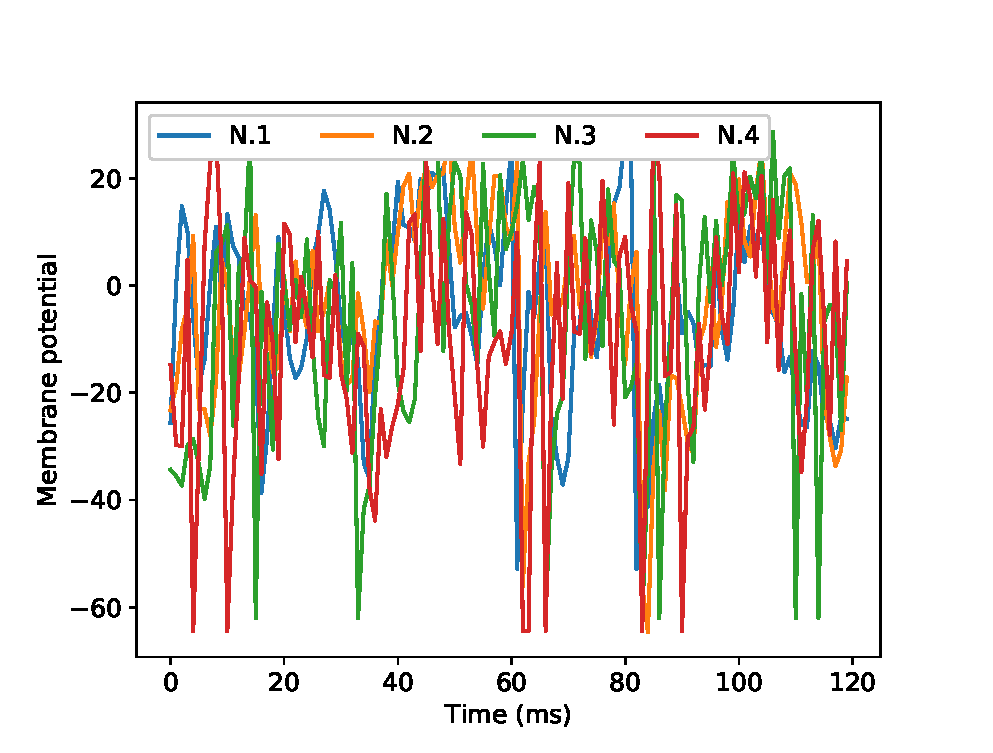
\includegraphics[width=0.7\linewidth]{figures/samples/membrane_potentials/export_sample_LIF_white_noise.eps}
    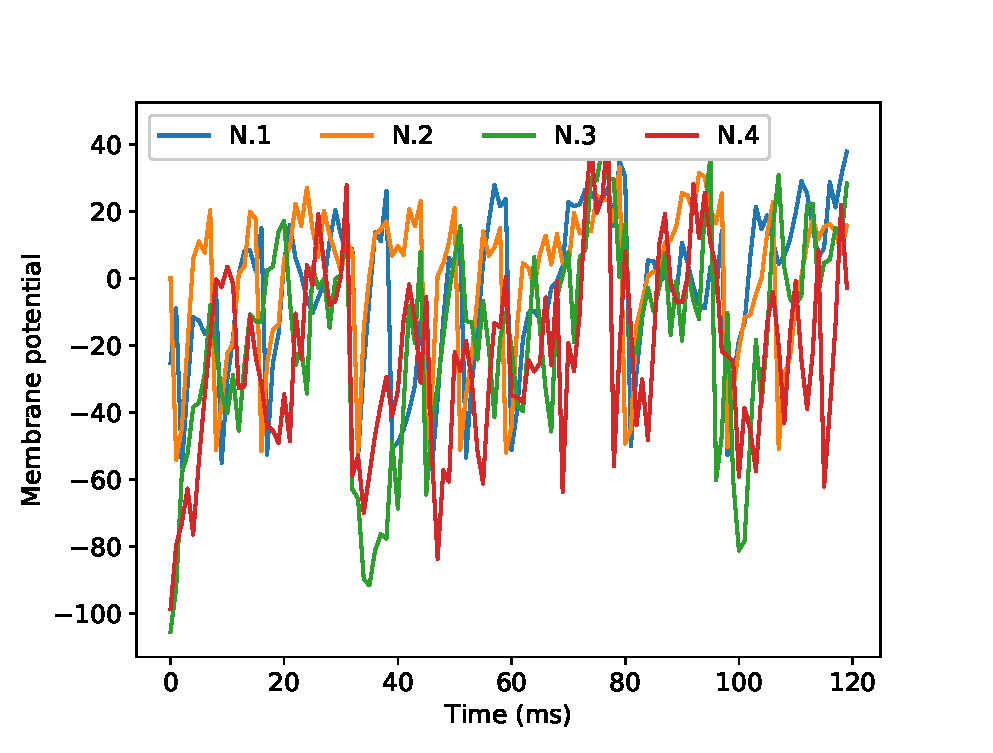
\includegraphics[width=0.7\linewidth]{figures/samples/membrane_potentials/export_sample_GLIF_white_noise.eps}
    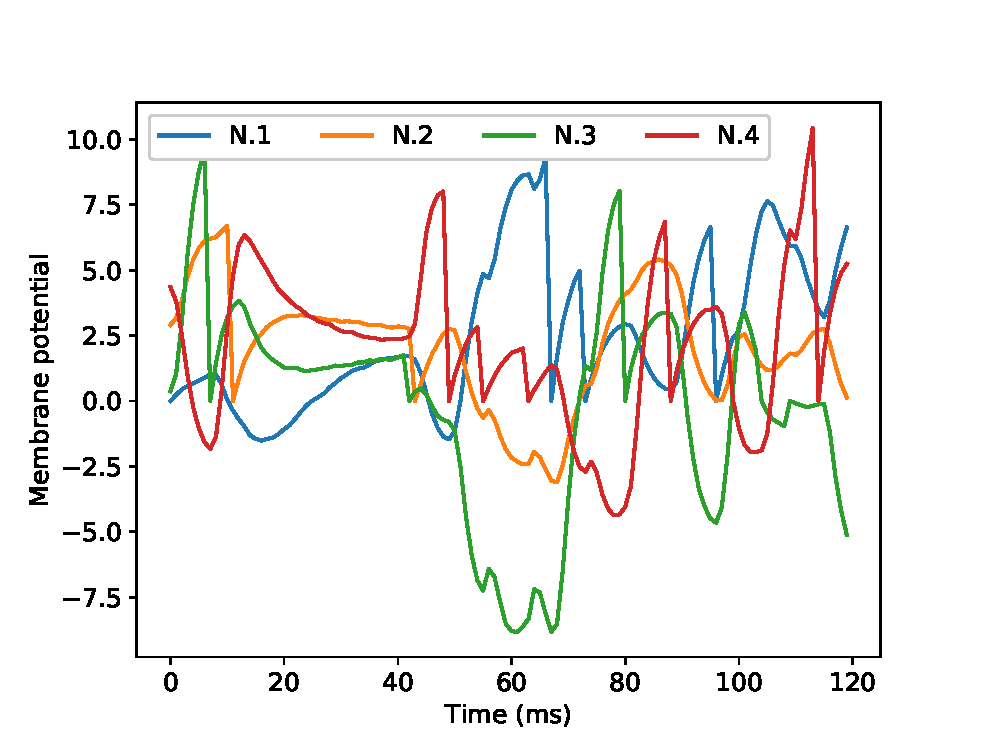
\includegraphics[width=0.7\linewidth]{figures/samples/membrane_potentials/export_sample_mesoGIF_white_noise.eps}
    \caption{Sample membrane potentials for a LIF, GLIF, and SGIF model - top left, right, and bottom, respectively, illustrating the slightly different nature of the time series across the model systems. Each line represents the membrane potential of a single neuron.}
    \label{fig:membrane_potential_samples}
    \vskip -0.2in
\end{figure}

\subsection{LIF}

% Write out definition, discuss a bit..? Refer to paper.
% Included portion of paper:

The neuron model we employed in this work is the leaky integrate-and-fire (LIF) model, as described in among other works \cite{Rolls1998Book}, and also in 
\ref{chpt:LIF}. For the sake of consistency, we include a brief description here in this chapter. The LIF model may be formally outlined as,

\begin{equation}
    \frac{dv}{dt} = \frac{E_L - v_t + R_I I_t}{\tau_m},
\end{equation}

where $E_L$ is the rest potential, $v_t$ is the membrane potential at time $t$, $R_I$ is the membrane resistance, and $I_t$ is the synaptic current.
The modelled networks are non-transitively fully connected (i.e. all-to-all connected, but with no self-recurrent connections), with the weights normally distributed between $w \in [-1, 1]$. The synapses are modelled as exponentially decaying post-synaptic currents, where a conductance variable $g$ models the conductance for the neurons,

\begin{equation}
    \frac{dg}{dt} = -\frac{g}{\tau_g},
\end{equation}

where the synaptic input current to a neuron $j$ is modelled as $I_{syn,j} = \sum_{i} w_{i,j} I_{i,j}$.

While forward passes are done according to a spike-threshold function with non-linear resetting of the membrane potential upon spiking, the backward pass is made possible by separately defining a differentiable soft-threshold function over the membrane potential which is used solely for back-propagating the error gradients obtained by minimizing the loss functions. We use the commonly applied sigmoidal function for this purpose,

\begin{equation}
    s_t(v) = \frac{1}{1+e^{-v_t}},
\end{equation}

where $s_t$ denotes whether a neuron spikes at time $t$ with a membrane potential $v_t$.
This results in that optimization of defined loss metrics always back-propagates error gradients through the soft-thresholded membrane potential, in effect treating this as a continuous spike value. 
In other words, the distance metrics calculate the distance between a continuous spike train to a binary target spike train.
Note that this also results in that sub-threshold values result in a spike signal during optimization.

% TODO: Update.
% \begin{figure}
%     \centering
%     \vskip -0.1in
%     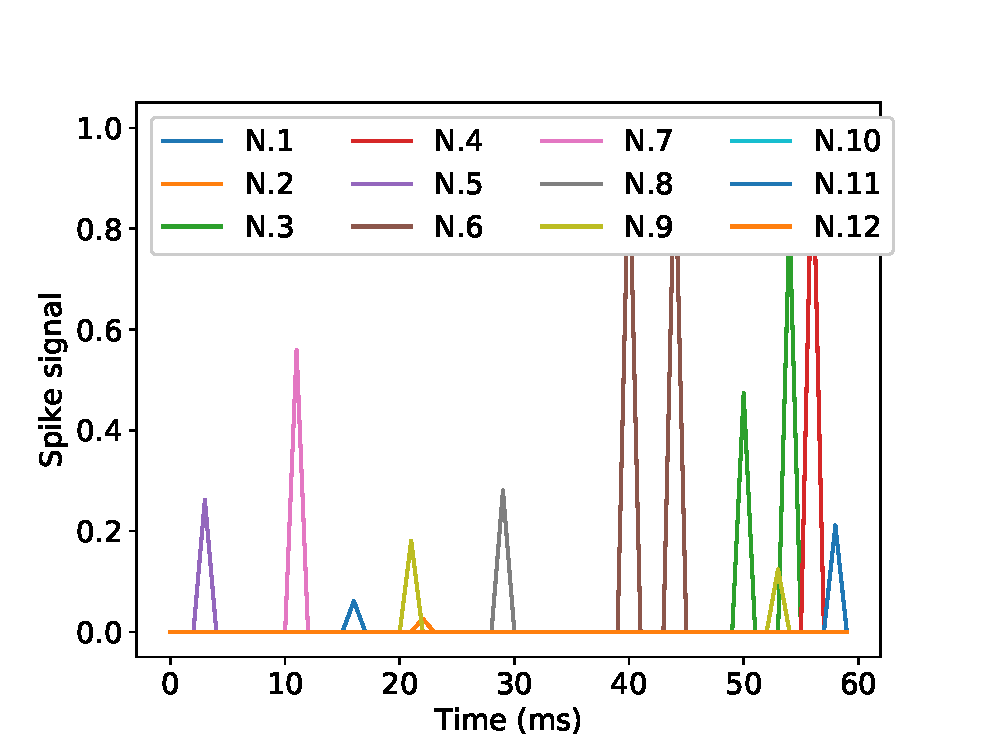
\includegraphics[width=0.9\columnwidth]{figures/plot_spike_thresh_lif_ensembles_dales_0.eps}
%     \vskip -0.1in
%     \caption{The soft-thresholded spike signal $s_t(v)$ for $60 \si{\ms}$ backward passes during model simulation for $12$ neurons.}
%     \label{fig:spike_thresh}
%     \vskip -0.2in
% \end{figure}

All parameters were held as free parameters during optimization, resulting in 4 $N$-dimensional free parameters, and one $N^2$-dimensional parameter, where $N$ is the number of neurons in the network. 


\subsection{Generalised leaky integrate-and-fire (GLIF)}

Our GLIF implementation is based on the whitepaper of \cite{allen_glif_white_paper}, and may be defined as

\begin{equation}
    \frac{dv}{dt} = \frac{g (E_L - v) + R_I I_{syn}}{C_m},
\end{equation}

where $v$ is the membrane potential, $g$ the conductance, $E_L$ the reversal potential, $R_I$ membrane resistance, $I_syn$ the total incoming synaptic current, and $C_m$ the membrane capacitance.
While the neuron model differential equations are linear, spiking is highly non-linear, and determined by the composite spike threshold $\theta_v + \theta_s$, whose differential equations are

\begin{equation}
    \frac{d\theta_v}{dt} = a_v (v - E_L) - b_v (\theta_v - \theta_{inf})
\end{equation}

\begin{equation}
    \frac{d\theta_s}{dt} = - b_s \theta_s
\end{equation}

where $\theta_v$ is a membrane potential dependent spike threshold, and $\theta_s$ is an exponentially decaying threshold, $a_v$ is an adaptation factor for $\theta_v$, $b_v$ is a voltage-induced threshold time constant, and $b_s$ is a spike-induced threshold time constant.
Introducing these thresholds makes spiking highly adaptive, which may mimic the temporal dynamics of the sodium-potassium pump, whilst remaining linear and differentiable.
Upon $v \geq \theta_v + \theta_s$ spiking occurs, which results in non-linear variable resetting, defined as,

\begin{equation}
    v_{\text{reset}} = E_L + f_v (v - E_L) - \Delta_V
\end{equation}

\begin{equation}
    \theta_{s,\text{reset}} = (1 - b_s) \theta_s + \delta_{\theta_s}
\end{equation}

where $f_v$ is the pre-spike voltage fraction influence on the reset potential, and $\Delta_V$ is voltage addition following reset.

Each neuron is connected to every other neuron in the network, the weights being normally distributed with values $w \in [-1, 1]$. The synaptic currents decay with a factor $f_I$ with an additive after-spike current $I_A$. This may be written as,

\begin{equation}
    I_{syn} = \begin{cases}
        (1 - f_I) I_{syn} + I_A, & \text{for } v \geq \theta_v + \theta_s \\
        (1 - f_I) I_{syn}, & \text{otherwise}
    \end{cases}
\end{equation}

where the synaptic input current to a neuron $j$ is modelled as $I_{syn,j} = \sum_{i} w_{i,j} I_{i,j}$.

GLIF neurons certainly allow for more biological realism in that they may exert most types of behaviour as outlined in the table in figure 2. in \cite{Izhikevich2006}.
As such, their information processing is theoretically greater, and the types of spike patterns they may exert are richer than when compared to LIF SNNs.


\subsection{Non-leaky integrate-and-fire (NLIF)}

% Refer to \cite{Huh2017}, mention impact, refer to synapse chapter.
Interestingly, using sub-threshold synaptic currents as the spike signal, rather than a surrogate function over the membrane potential, results in not only a continuous optimisation signal, but also one that has a specific temporal signature, depending on neuronal excitation.
Extending the work of \cite{Huh2017}, we implement first their non-leaky integrate-and-fire (NLIF) neuron model, with the aforementioned sub-threshold synapse model, which is defined using a gating-function which essentially results in a synaptic current when the potential is inside of an active zone.

\begin{equation}
    \int s dt = \int g dv = 1,
\end{equation}

where $s$ is the synaptic currents, and $g$ is the current gating function, and the synapse model is,

\begin{equation}
    \tau_s \frac{ds}{dt} = -s + g \frac{dv}{dt}
\end{equation}

Combined with a lower-dimensional target signal this enables perfectly learning to perform the task, albeit with the inferred model parameters depending largely on the initial configuration and random seed.
We extend their work to also test their methodology on LIF SNNs (see chapter \ref{chpt:frontier}, and find that although this results in non-exact gradient calculation, the setup is sufficient for inferring models with near-perfect performance in reproducing the target signal for LIF SNNs, too.

\subsection{Stochastic integrate-and-fire models (SGIF)}\label{microGIF}

Lastly, to tie my work with a current state-of-the-art procedure, we have implemented the cortical microcolumn-inspired (based on \cite{Schwalger2017}, adapted to a lower set of neurons) stochastic integrate-and-fire (SGIF) population model of \cite{Rene2020}, and extended it such that it is compatible with in-place gradient based optimisation. 
We compare the results on both population- and neuron-level model fits with previously reported results, and also propose that the GBO procedure may be used to directly infer heterogeneous neuron-level models, and test this by fitting models to a full-size SNN SGIF target model.
We also test fitting SGIF models to biological data, and evaluate the goodness of fit using loss metrics and geodesic similarities between the NMF modules.

While we refer the reader to \cite{Rene2020} for the full model definition, we wish to outline the crucial parts to making the models in-place differentiable - not requiring using approximate Bayesian computation over model samples in order to estimate a posterior.
The synapse model may be defined as,

\begin{equation}
    \tau_s I_{syn}(t) = W_{syn} \epsilon_s(t),
\end{equation}

\begin{equation}
    \tau_s \epsilon_s(t) = (1 + \tanh(t_{s} - \Delta_s)) e^{-\frac{t_{s} - \Delta_s}{\tau_s}},
\end{equation}

where $t_s$ is the time since the previous spike, $\Delta_s$ is the delay before synaptic transmission after spiking, $W_{syn}$ are the synaptic weights, and $\epsilon_s$ is the synaptic kernel, or spike-transmission model.
Note that the key difference between this formulation and the one in \cite{Rene2020} is using the $\tanh$-function to incorporate the transmission delay, rather than by using a Heaviside function $\Theta$, as this allows us to differentiate the function, and thus backpropagate error gradients to calculate parameter gradients.
Thus, we may use negative log likelihood estimation over the spike probabilities, i.e. maximising the likelihood that a set of spike probabilities produce the target spike trains when drawing from a Bernoulli distribution with the probabilities, which is equivalent to minimising the negative log likelihood of the target spike train given simulated probabilities.

% Based on the work of \cite{Rene2020}, which is based on \cite{Schwalger2017}.
% Spike probability, rather than membrane potential and spikes.
% --> Minimise negative log-likelihood under a Bernoulli or Poisson assumption.

% ALlows for a direct comparison.


% % TODO: check: "frontier" found using frd - vrd obscures gradient and diverges more.
% BNLL \& PNLL "frontier"

% \subsection{GLIF neurons}
% Can be highly parameter-sensitive and result in completely different mode of neuronal behaviour


\section{Loss metrics}

% simple, rate-based metric. does not capture correlations, or only very vaguely if done over smaller time bins. 
% can be combined with correlation metric.

% Tricky design, stochasticity, lots of considerations, as we shall see only frontier..
Designing suitable loss metrics is one of the main challenges in applying gradient based optimisation to SNNs, as it is what defines the gradients, and thus the parameter space that we traverse during and throughout optimisation.

We performed optimization using (1)~the firing rate distance, (2)~the van Rossum distance, and (3) the negative log-likelihood assuming either a Bernoulli or Poisson PDF for the probabilistic models.
Further, we performed initial testing using an additive combination of the van Rossum and firing rate distance, a Pearson correlation metric distance, the Fano Factor \cite{Tchumatchenko2011, Kreuz2013a}, and the mean squared error, but found empirically that none of these were able to produce good results in terms of convergence or performance, and thus abandoned testing the metrics further for this project.
Reasons for why these we unsuccessful may partly be explaiend by the reasons outliend in the van Rossum distance section below.

\subsection{Firing rate distance}

We define the firing rate distance as the Euclidean distance between each neuron's average firing rate for a given spike interval, which may be written as,

\begin{equation}
    d_r(S_1, S_2) = \sum_i^N{\frac{\sqrt{(s_1^i - s_2^i)^2}}{\Delta t}},
\end{equation}

where $s^i$ is the number of spikes for neuron $i$ in a given interval $\Delta t$.

\subsection{van Rossum distance}

\begin{figure}
    \centering
    \vskip -0.1in
    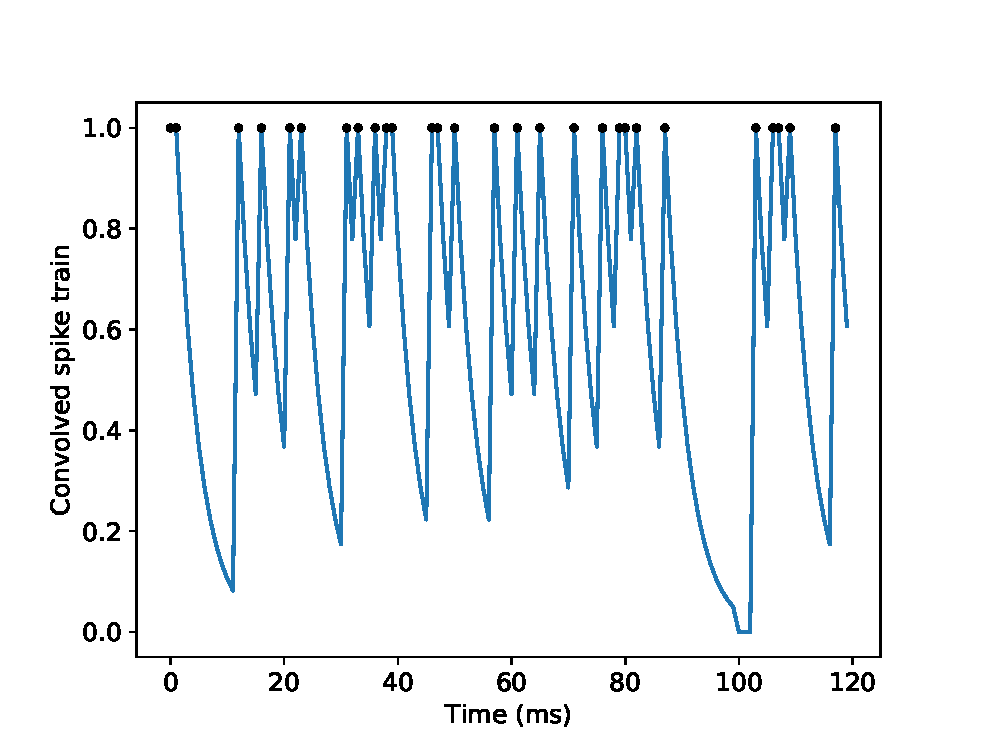
\includegraphics[width=0.8\columnwidth]{figures/samples/neur_vr_conv_sample.eps}
    \vskip -0.1in
    \caption{An illustration of the van Rossum convolution over a sample spike train.}
    \label{fig:vrd_conv_sample}
    \vskip -0.2in
\end{figure}

One thing is quantifying distances in terms of spike metrics.
Another is designing a metric that is well-defined for gradient-descent.
While the van Rossum metric describes the distance between two spike trains both in terms of rates and timing, due to its sensitivity to exact timing the gradient signal might be obscured for non-matching neurons, and more well-defined where the rates better match.

The van Rossum distance \cite{VanRossum2001} may be defined as the Euclidean distance between two spike trains where each spike is convolved with an exponential kernel, see figure \ref{fig:vrd_conv_sample}, forward in time,

\begin{equation}
    f_{conv}(t, t_{i, spike}) = e^{\frac{-\Delta t_i}{\tau_{\mathrm{vr}}}}
\end{equation}

where $\Delta t_i = (t-t_{i, spike}),\ t \geq t_{i,spike}$, 
with $t$ being the current time, $t_{i,spike}$ the most recent time of spiking for neuron $i$, $\tau_{\mathrm{vr}}$ a time constant (set to $\tau_{\mathrm{vr}} \in \{10.0, 20.0, 100.0\} \si{\ms}$ in the experiments, and $\Delta t_i$ the time since the neuron's last spike, $\Delta t_i = (t-t_{i, spike})$, the distance between two spike trains is then given by the Euclidean distance between two convolved spike trains,

% potential figure of convolved spike train?

\begin{equation}
    d_v = E(S_1, S_2) = \sum_{t=0}^{t=N} \sqrt{(f_{conv}(S_1)-f_{conv}(S_2))^2}
\end{equation}


Our initial hypothesis was that using the van rossum distance, we may better 'guide' the parameter inference search in the parameter traversal in the error landscape (then provided by the van Rossum distance metric), allowing gradient-based methods to converge more often, and to better solutions.
The basis for the hypothesis was that using the van-rossum distance as a loss function for the spike trains, we attain a more continuous signal, since the discrete spike train is convolved with a time-based kernel, whic may make the gradients more informed via the loss function in larger search areas.
However, our findings contrast this hypothesis, and we find "\textit{wandering gradients}" for the van Rossum distance.
Wandering gradients may be defined as gradients that point in no consistent direction, but results in that parameters "wander" arbitrarily during optimisation, in our work due to being in a region for which the loss is relatively constant and uniform.
Upon closer inspection, the spike train data sets have a too high variability for an emphasis on the precise timing to improve optimisation performance - and we end up only obscuring the error signal further by using the van Rossum distance. 
I.e. it breaks down for the stochastic signals, and only works well for NLIF, or when we increase the time-constant such that the metric approaches a rate-based metric. And even then the firing rate distance might outperform the van Rossum distance metric for the surrogate gradient descent approaches.


\subsection{Maximum Likelihood Estimation}

% Negative log-likelihood (Bernoulli, and Poisson PDF assumptions) for probability-based models.
By assuming either a Bernoulli or Poisson distribution for the observations, or spike trains, we can maximise the likelihood of producing that same data by using numerical methods.
As usual, it is easier to work with a sum of products, rather than exponents, when doing numerical differentiation over a probability distribution to find the maximum likelihood estimate (MLE).
Therefore we maximise the log-likelihood over the distribution, as it lets us work with a sum of products instead of a product of exponential functions, and is equivalent to maximising the likelihood itself.
In fact, we also instead minimise the negative log-likelihood, which remains equivalent to maximising the likelihood, as this lends itself directly to optimisation as a loss metric and error signal which may be used for gradient-calculation.

\begin{equation}
    \mathcal{L}(\theta | x) :\propto - \log \mathcal{L}(\theta | x) = - \log \prod_{n=1}^N pdf(\theta; X) = - \sum_{n=1}^N \log (pdf(\theta; X))
\end{equation}

Assuming a Bernoulli distribution, $pdf=Bernoulli(\theta; x)$, or assuming a Poisson distribution, $Poiss(\theta; x)$, these let us estimate the maximum likelihood over $\theta$.


\section{Summary}

This chapter outlines SNN models and gradient based optimisation, and contextualises the model class and inference methodology combination in the field by drawing parallels to probabilistic models, RNNs, and machine learning.
A few selected key works is briefly presented and discussed, before background material relevant for SNN model evaluation is presented, along with a proposed baseline model; the GLM.
Further, various SNN models are presented and formally defined, as well as the probabilistic SGIF model, which allows us to draw parallels to published work that used ABC and MCMC sampling for the SGIF SNN.
Lastly, the two main loss metrics used in GBO for SNNs are presented, along with MLE for probabilistic models as is widely applied in ML.
This provides the basis for implementation of the outlined models and procedures, which is presented throughout the remaining chapters of this thesis.

The goal in this thesis is to test the hypothesis that gradient-based optimisation may be used for spiking neural networks to capture higher-order statistics, including ensembles of activity on the network level, and to test whether ground-truth parameters can be retrieved using the approach.
We implement a modular GBO framework in PyTorch, along with several different types of SNNs and loss metrics, which lets us test the aforementioned hypotheses, as well as to perform further implementation of the subthreshold currents synapse model of \cite{Huh2017} in order to test whether ground-truth could not be retrieved due to unknown model input or training pattern complexity, as well as whether this more continuous model output implementation would provide a better basis for GBO. The latter turned out to be the case, with excellent convergence and task performance was observed, also for a leaky IF-implementation where exact gradients were thus not computed for BP in the model. However, ground-truth parameters were still not retrieved.

To sum up, some of the key contributions of this thesis includes:

\begin{itemize}
    \item Showing that there is a near linear relationship between the recovery variables of the Izhikevich model and the resulting SNN firing rate
    \item Showing that LIF SNN inference using GBO is attainable, and that Adam may be a better optimisation strategy than SGD
    \item Finding that the van Rossum distance may make optimisation diverge in the case of using noisy, uknown input, due to the emphasis on precise timing, which is not meaningful in this case
    \item Demonstrating and providing a modern, modular and efficient implementation of SNN inference in PyTorch, which is modular wrt model, loss metric, and optimiser
    \item Proposing batching as a means of ameliorating the on-line constraint of SNNs due to parameter state dependence
    \item Coupling our SNN model inference work with published work on SGIF models and ABC
    \item Coupling SNN inference with SNPE, finding that posterior-estimation over all parameters might not be meaningful and not well capture the ground-truth means, due to the multiple solutions in parameter-space
    \item Finding that we cannot hope to retrieve the ground-truth parameters, and that this might not be a meaningful goal when aspiring to capture the target spike data
    \item Finding that we may capture higher-order statistics in terms of the NMF module similarity in our SNN models when using GBO, also beating or being on par with the proposed GLM baseline models
    \item Finding that even for the case of a non-noisy, fixed, lower-dimensional encoding-task, we converge towards completely different SNN model parameters, all with excellent task performance, even when employing continuous sub-threshold synaptic current models, strengthening the hypothesis that aiming to retrieve the ground-truth parameters might not be meaningful
    \item Finding that the methodology of \cite{Huh2017} is applicable to leaky models, by extending their work on non-leaky integrate-and-fire models
\end{itemize}


% =======================================================

\chapter{Complementary poster: Izhikevich recovery variable parameters, oscillations and resulting network rates}\label{chpt:izhikevich}

In our initial SNN research, we replicated \cite{Oliveira2019} to show that the resulting rates could be formulated more or less as a linear function, resulting from sub-threshold oscillations, and that the model is highly sensitive to its initial parameter values.
One of the motivations for doing this was that the model class may exert all neuronal modes of behaviour as observed in biology \cite{Izhikevich2006}.
However, as hinted to above, this results in a highly irregular parameter landscape, only further complicated by the previously discussed stochasticity present in the model inference scheme that we are studying.
To give an intuition about why this is, consider that the Izhikevich model is a 2-dimensional projection of a 4-dimensional ODE system - in fact based upon the original HH model \cite{HH1952}.
As such, there are regions for which unstable, or even chaotic behaviour, may emerge - i.e. we end up with parameter regions for which the model is highly unrealistic, or not well-defined.
Therefore, we limit our research to the previously outlined models, and only include parameter landscape plots illustrating the aforementioned, as well as our work on the effect of the recovery variables on resulting subthreshold oscillatory behaviour.

% TODO: Include param landscape figures here??

% All modes of behaviour as observed in biology, however something needed to shift mode(s) of behaviour..
% Parallels to SNN inference etc
% (2D ODE syst per neuron)

\section{Poster: \textit{The effect of the recovery variable parameters on oscillating Izhikevich networks}}\label{section:izhikevich}
\includepdf[pages=-]{files/berg_and_onken_uk_neural_computation_2019_poster.pdf}


% Result of sub-threshold oscillations. 
In sum, although the Izhikevich model is capable of almost all types of behaviour as seen in biology with only 2-dimensional ODEs per neuron, it comes at the cost of also being able to exhibit highly unrealistic, or chaotic behaviour, for which GBO would diverge, as gradient would be completely un-informative.
Further, there is a strong dependence on a sub-set of the model parameters, which also poses an issue for GBO; these are the only parameters likely to be inferred using GBO unless specific design and care is taken to calibrate the other parameters, such as for instance sequentially after initial inference of the others - however, this would then render the other inferred values completely dependent on the variables inferred prior in the sequence. 
In some preliminary experiments we confirmed empirically that divergence indeed did occur due to chaotic behaviour, which was not easily avoided due to several regions of parameter hyperspace for which such behaviour can occur. 
As such, Izhikevich SNNs are not used further in thiswork where we study SNN inference using GBO.


% =======================================================
\chapter{Gradient-descent based LIF SNN inference}\label{chpt:LIF}

\section{Poster: \textit{Spiking Network Inference Using Gradient Based Optimisation}}

Before beginning on the next chapter, which describes in more detail the state-of-the-art of SNN inference using both gradient-based optimisation and to some extent approximate Bayesian computation by simulation-based inference, we would like to present the work that we have done specifically for and constrained to leaky integrate-and-fire neurons using gradient-descent for parameter-inference, before expanding on the methodology and applying it to a wider range of model types and classes in the following chapter \ref{chpt:frontier}.
The poster contains the essentials pertaining to the post-inference NMF analysis, the van Rossum distance metric, as well as single-neuron level rate analysis, along with inferred kernel density estimates over the parameters across experiments.

These experiments seemed highly promising with regards to ground-truth parameter retrieval - however, they are in part due to smaller initial parameter intervals, and the fact that the LIF-model is relatively low-dimensional.
This becomes clearer in the more extensive report on LIF inference when considering the relative (normalised) parameter distance before and after training, which was done following the work presented in the poster.
It is nevertheless interesting that the inferred kernel density estimates are somewhat centred around the true means for several of the LIF-parameters.
While we hypothesise that this won't hold for the more high-dimensional models, such as for the stochastic general integrate-and-fire (SGIF) \cite{Rene2020} and generalised leaky integrate-and-fire (GLIF) models \cite{allen_glif_white_paper}, it is certainly something that it would be interesting to pursue in future research.

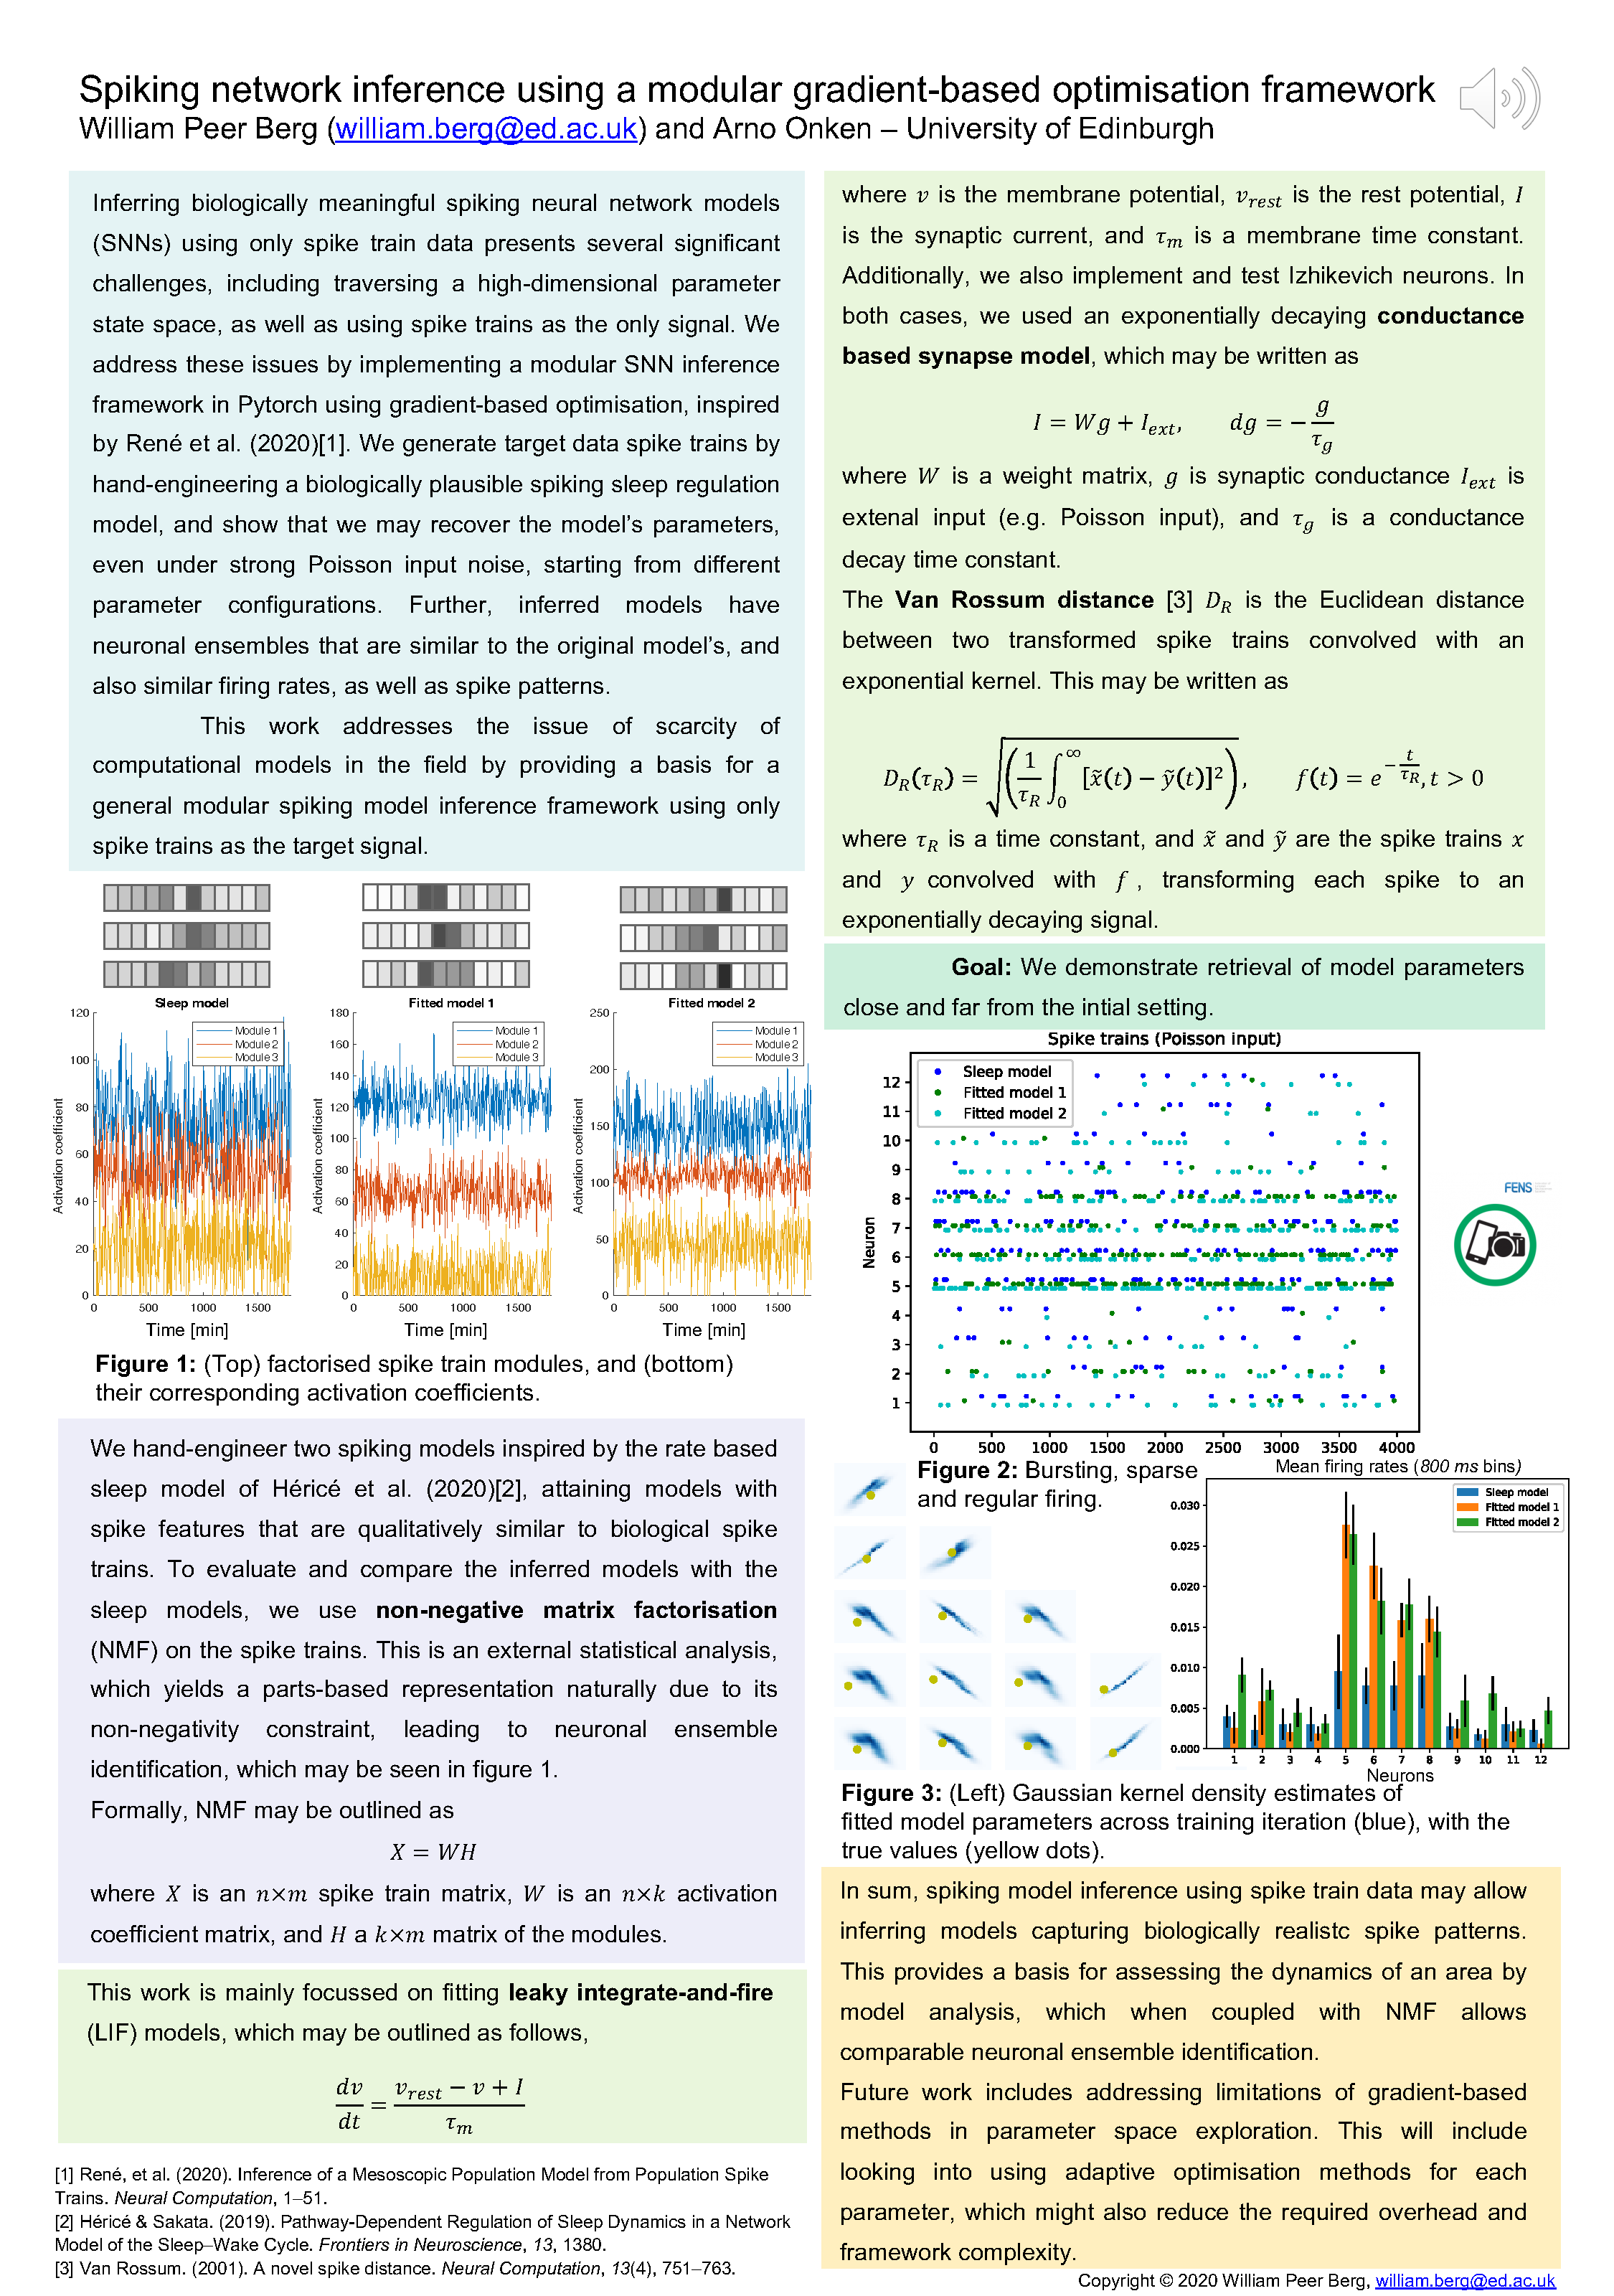
\includepdf[pages=-]{files/FENS-virtual-2020-e-Poster-W-P-Berg-and-A-Onken-Spiking-Network-Inference-Using-Gradient-Based-Optimisation-PORTRAIT-5.pdf}

\section{Report/paper draft: \textit{Parallel spiking neural network parameter inference using gradient based optimization}}

The report addresses different combinations of the van Rossum distance and firing rate distance metrics, as well as different optimisation schemes.
These did not vary significantly for the LIF model, at least not when considering the relative (normalised) parameter distance and geodesic NMF model similarities between stochastic gradient descent (SGD) and adaptive moment estimation (Adam) optimisation, nor between the van Rossum distance and firing rate distance.
This may suggest that the lower dimensionality of the LIF model results in that all setups are rendered "good enough" for the model inference.
As we shall see in the following chapter, specifically in the subsection on error and parameter landscapes \ref{sect:e_landscapes}, the reason for this is that the loss metrics result in regions in the parameter error landscapes for which the error and thus gradient is unchanged.
However, during our work in the next chapters, we observed empirically in initial experiments that Adam was significantly better in terms of both convergence and the number of training iterations for the more complex models (SGIF and GLIF), as well as in the gated subthreshold synaptic current synapse models in chapter \ref{chpt:gated_synaptic} \cite{Huh2017}.
One possible explanation for this is simply the same as in the ML domain; the adaptive moment allows for an adaptive response to the gradients, and is lowered when the gradient rate of change does not.
In our case, i.e. for LIF models, this does in effect only gain the benefit of being able to converge without too much calibration of the learning rate, as this is adapted throughout inference.
In effect this may be seen as a type of simulated annealing, only relative to each parameter and their gradients.

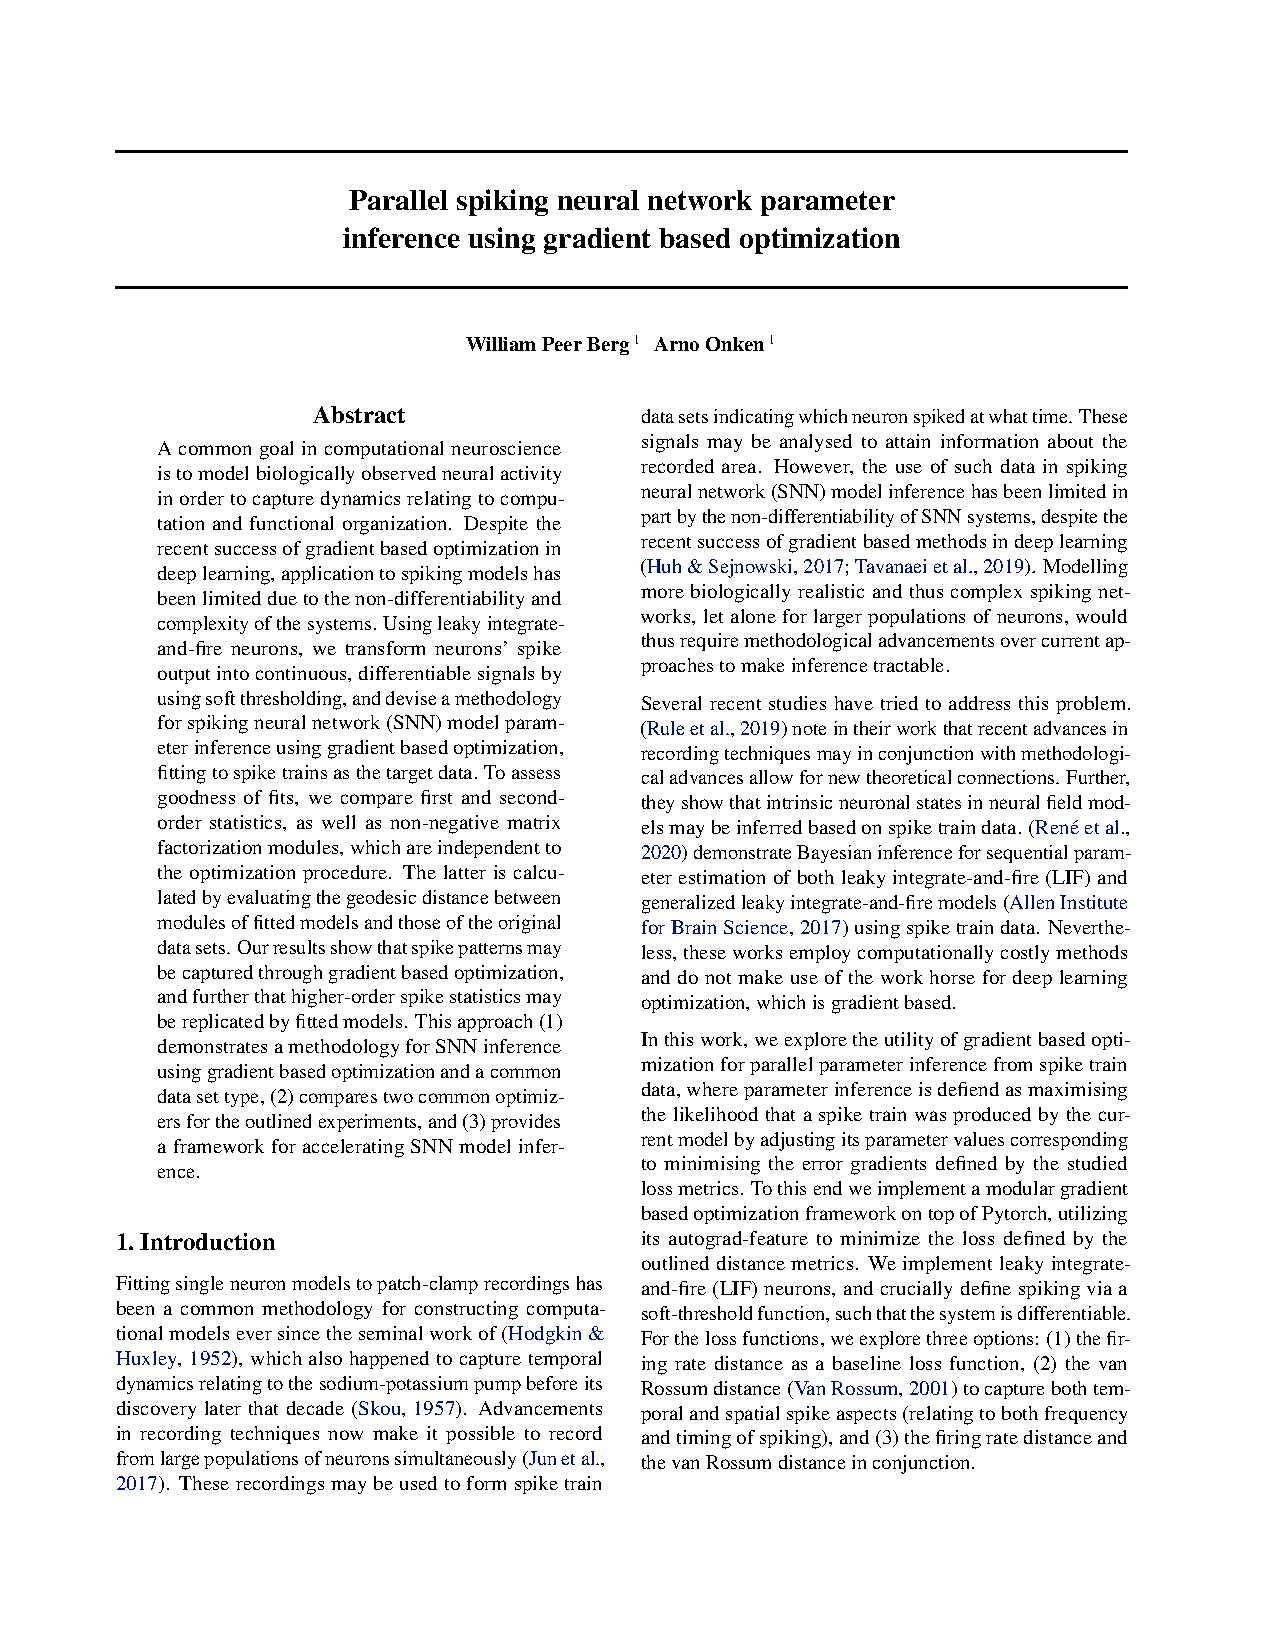
\includepdf[pages=-]{files/icml2021_draft_snn_inference_berg_onken.pdf}


This report provides the basis for SNN inference using GBO, different loss metrics and optimisers for the case of LIF SNNs, and also presents a way of evaluating the goodness of fit using NMF, comparing with GLMs as a baseline model.
This is the foundation upon which the rest of the work in this thesis is based on, and expands on.
In the rest of this thesis, we consider the case of using the Adam optimiser with different classes of SNNs and either a rate-based loss metric over intervals of spikes, the van Rossum distance, or the negative log-likelihood where considering probabilistic models.
As no significant performance gain was observed when using a combination of the two metrics was observed, this is not used in further GBO work using other SNN models.
In fact, as we shall see, when increasing the model complexity, the fact that the van Rossum distance may emphasise the timing of spikes in such a way that the gradient may be obscured, may be disastrous on inference, resulting in divergence.


% =======================================================
\chapter{The frontier of SNN inference}\label{chpt:frontier}

In order to study how to infer spiking neural network models (SNNs) we need several ingredients: (1) a definition of the system, (2) an algorithm for model inference, and (3) an implementation of (1) and (2), where the algorithm for the case of gradient descent also necessarily contains (3) a way to measure and assess model performance, which is ideally comparable with existing methodologies and models.

Research on SNNs using gradient-based optimisation is fairly limited, and includes approximate Bayesian computation for smaller models, conversion learning in which more traditional ANNs are transformed to simpler SNNs after training, or surrogate gradient descent, in which a surrogate signal over the model spikes, usually as a function over the membrane potential, is used in order to obtain a differentiable output that may be used to optimise the model's parameters over a given loss metric by backpropagating the error signal. Notably, there exists some research on gradient descent for SNNs in which the model is defined such that its parameters may be used directly for error signal gradient backpropagation, including \cite{Huh2017}, \cite{Rene2020}. This is slightly different from surrogate gradient descent in that the backpropagation is a more natural extension of the system, and thus albeit remaining unrealistic in terms of biology, it is closer to learning in a Hebbian and spike-time dependent plasticity (STDP) fashion, as noted by the authors in \cite{Huh2017}.

% Currently, the state-of-the-art methods are only partly successful in training a subset of SNN model parameters for smaller models.
With the goal of accelerating SNN inference research, we looked at the most prominent state-of-the-art methodologies for SNN inference, which may be divided into (1) gradient based optimisation (GBO), and (2) approximate Bayesian computation (ABC) \cite{Lueckmann2018, Rene2020, Cranmer2020a, Lueckmann2021}.
GBO enables leveraging recent ML advances from deep learning, and albeit biologically implausible as a learning rule in its own right, allows for in-place inference of models that are biologically realistic. The computational cost of doing gradient based computation is also exponentially less than that of doing ABC, as this involves doing a costly (Monte-Carlo) sampling step \cite{Rene2020}.
Therefore, GBO is the main focus of this work, and leveraging system definitions that may allow for more information to be captured and propagated by means of gradient descent types of optimisation is therefore also something that is desirable, and notably consistent with the works that have been extended.

As for ABC, Bayesian inference has until recently been intractable for SNNs due to their high-dimensionality. However, recent advances in deep learning, leading to the advent of sequential neural posterior estimation (SNPE) \cite{Greenberg2019a, Durkan2018, Goncalves2019, Cranmer2020a}, in which a DNN is trained to estimate a posterior over a prior given observations, has allowed for much more efficient sampling using this amortised approach; sampling from the DNN to perform posterior parameter estimation (which in turn uses GBO in the posterior inference, i.e. for fitting the DNN).
Note however that this procedure still has a high cost due to the sampling procedure, and does not scale well with an increase in the network size.
% references, brief summary and discussion of main references
Using a Bayesian approach, we may however estimate the posterior over the model parameters, given our approximation of the prior. This also yields a type of uncertainty estimate around the posteriors. Note however that the posterior will be skewed by the prior approximation, in our case given by SNPE.
 
Using a surrogate gradient approach, we may fit the parameters of the system by error minimisation using a differentiable loss function. 
By working with biological spike train data, which is a very widely used format, we cannot however make many assumptions about the input, unless the recording somehow also contains information about this signal. 
Therefore, we have to model the input in some way, taking care in considering how assumptions may affect model behaviour during learning. 
As a rule of thumb, we want to have a signal which allows for the network to perform the task at hand, or to replicate the observed data, whilst remaining biologically reasonable.
In other words, we want to have input that puts the system in a realistic mode of behaviour, and yet allows us to optimise its parameters.
This means providing an informative signal, which is meaningfully transformed by the model with regards to output error minimisation, and thereby also usable in this regard.
% As it is limited what we may assume about the input, loss metrics that put a high emphasis on the precise timing of spiking may in fact obscure the gradient signal by incorporating too much of the noise stemming from this signal.
% We therefore focus on metrics that are more rate-based, looking at intervals of spikes in order to include the temporal signatures to some extent.
% Using a timing-oriented metric over larger time bins may even result in divergence, due to variability between the hidden target data input, and the inferred model input. 


% \section{My contribution: Implementing, differentiating and optimising different SNN models using different loss metrics}
\section{GBO compatible SNN framework in PyTorch}

% TODO
% Goals and questions or hypotheses

In order to test the extent to which gradient based optimisation may be leveraged for spiking neural network model inference, we have developed and implemented a novel framework in PyTorch \cite{Paszke2017, Paszke2019}.
It allows performing gradient descent over a specified loss metric, for any differentiable SNN model definition, in a highly modular way.
We have implemented a surrogate gradient approach over the membrane potential itself for LIF and GLIF neurons with rate-based metrics as well as spike-time dependent metrics, and over the spike probabilities by using the negative log-likelihood for SGIF neurons, as well as for non-leaky integrate-and-fire neurons by directly using the synaptic currents as readout signals, and considering a more high-dimensional output target signal.
Notably, we extended the latter synaptic current model, as originally presented by \cite{Huh2017}, and combined it with leaky integrate-and-fire models, for which optimisation was highly successful. The work with the synaptic current modification is presented later in chapter \ref{chpt:gated_synaptic}.
% As spikes are binary in nature, by implementing surrogate subthreshold spike signals, we may facilitate optimisation, improving optimisation performance for gradient descent.

As for hypothesising the extent to which GBO may be used to retrieve model parameters that are close to the ground-truth values, we may assess this by fitting to synthetic data.
We hypothesise that we will retrieve local minima which is not close to the ground-truth values where this is accessible, but that the models will however capture the spike statistics to a large extent, potentially allowing for functional analysis and model probing for further hypothesising. 
This can be understood by considering the error landscapes formed by the loss metrics, which we shall plot later in this chapter in order to illuminate this.
Further, we shall also test the extent to which we have captured similar ensembles in the spike trains of the fitted models, by comparing the modules attained by non-negative matrix factorisation, a dimensionality reduction technique well suited for neural spike train analysis due to its non-negativity constraint, irrespective of the parameter values of the fitted models.

% As such, it may be used to evaluate the functional characteristics of the modeled nuclei.
% The input is unknown.
% SBI approach for SNN inference; limitations. Test potential.
% Better for true parameter estimation. However,  posteriors are probability densities, and do not have direct access to full model configurations as such, and may suffer from not capturing full specific model configurations that capture as many higher-order spike statistics.
As a baseline model for comparison in NMF module similarity, we use generalised linear models (GLMs) (see section \ref{subsect:GLMs}), which are good candidates for capturing spike statistics in the NMF analysis due to their exponential family (and here Poissonian) formulation.
However, we hypothesise that GBO for SNNs may enable capturing a higher factorised module similarity than the GLMs fitted by maximum likelihood estimation (MLE).
If so, this could either be due to an inductive bias (by model definition), or due to the richer range of behaviours available to the SNN models.
% Input transformation (?, avg. relative spiking per population ?)
% net(x\_forward)
% Output transformation (avg. v per pop.)
% Can transform spike-train to average population membrane potential
% Synapses with dg/dt ?
% self.g = torch.ones\_like(self.v)  for one conductance per neuron (for n synapses)

% \subsection{Contribution: PyTorch}

% ... tricks, sequentiality etc
Current implementations of SNNs in the field are commonly done in Brian 2 \cite{Goodman2008} or Matlab. 
Upon commencing work on SNNs using LIF neurons, the only recent work we found that supported optimisation in a supervised or semi-supervised manner was in Theano \cite{Bergstra2010}, a legacy Python library for symbolic programming.
With recent advances in ML not only through increased computational resources and novel optimisation techniques, but also in programming libraries that also compile to and run on the GPU, and in either case contains highly optimised library code implemented in a lower-level programming language (typically C, C++, or Cuda), we wanted to make use of this aspect too, and after too many hours of fighting with at best poorly documented legacy Theano-library code, we decided to set out to implement SNNs in PyTorch.
This led to the implementation of a modular framework and pipeline of SNN inference using GBO in PyTorch \cite{Paszke2017, Paszke2019}.
Key to allowing using PyTorch, is maintaining a neuronal state throughout simulation, which we implemented by enforcing sequential input propagation throughout the model, such that the internal state is updated for each time-step.
With this simple trick, intervals of input mutate the state with each input corresponding to some desired time-step constant, in my code set to $1 \si{ms}$ for simplicity.
However, it does result in that intervals of simulation need to be performed for each backward pass, i.e. updating the model parameters given error gradients.

\begin{figure}
    \centering
    \vskip -0.1in
    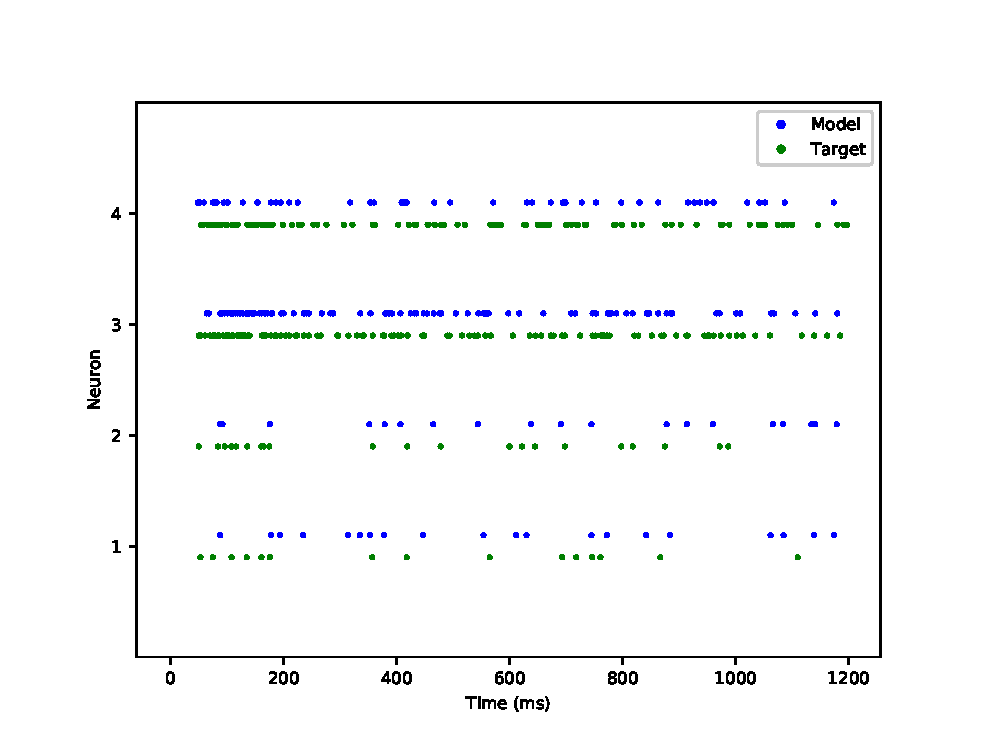
\includegraphics[width=\columnwidth]{figures/samples/SameModelClassTarget/export_spike_trains_euid_12-10_09-45-02-423.eps}
    \vskip -0.1in
    \caption{Target and fitted GLIF model spike trains for one of the GBO inference experiments when fitting to target spike train data generated by a hand-engineered GLIF SNN (green/bottom spikes in the spike train plot).}
    \label{fig:sample_GLIF_spikes}
\end{figure}

\begin{figure}
    \centering
    \vskip -0.1in
    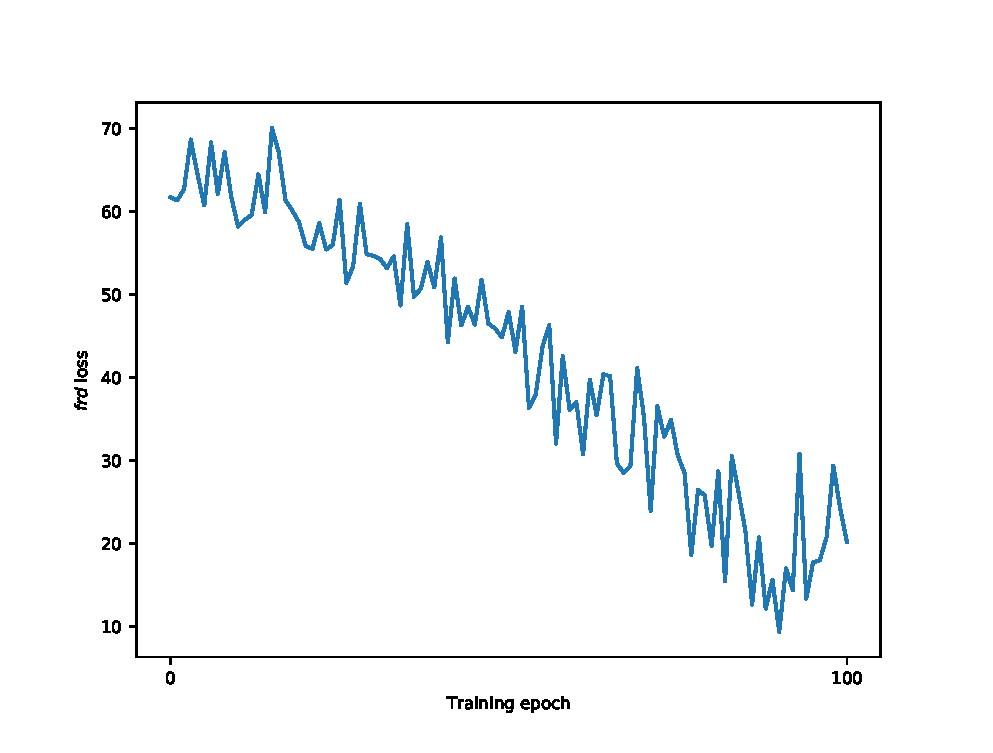
\includegraphics[width=\columnwidth]{figures/samples/SameModelClassTarget/export_GLIF_plot_loss_euid_12-09_16-17-13-464.eps}
    \vskip -0.1in
    \caption{Loss per training epoch for one of the GBO inference experiments, with the final model and target intervals plotted in figure \ref{fig:sample_GLIF_spikes}, and the membrane potentials in figure \ref{fig:sample_GLIF_vs}.}
    \label{fig:sample_GLIF_loss}
\end{figure}
    

\begin{figure}
    \centering
    \vskip -0.1in
    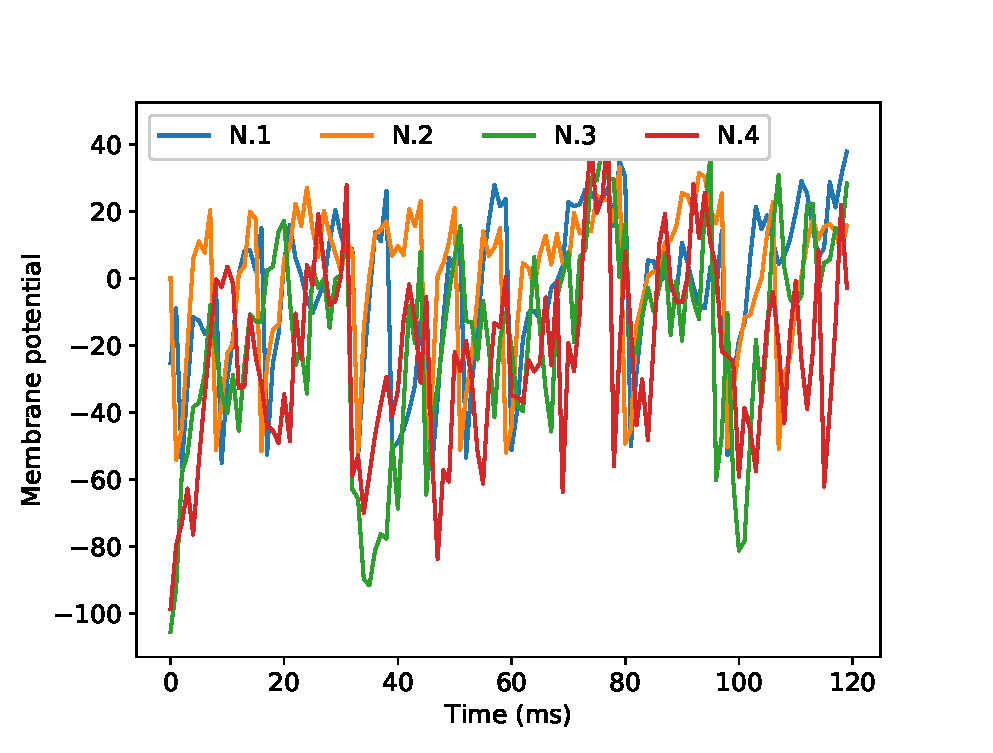
\includegraphics[width=0.7\columnwidth]{figures/samples/membrane_potentials/export_sample_GLIF_white_noise.eps}
    \vskip -0.1in
    \caption{The membrane potentials for the fitted GLIF model in figures \ref{fig:sample_GLIF_spikes}, \ref{fig:sample_GLIF_loss}.}
    \label{fig:sample_GLIF_vs}
\end{figure}

We implemented a general SNN optimisation framework on top of PyTorch \cite{Paszke2017, Paszke2019} and utilised PyTorch's autograd-feature for backpropagation of error gradients.
Key to enabling backpropagation is defining a differentiable output signal. Traditionally, the sigmoid function is a common choice, i.e.

\begin{equation}
    s_t(v) = \frac{1}{1+e^{-(v_t-(\theta_v + \theta_s)}}
\end{equation}

where $s_t$ denotes whether a neuron spikes at time $t$ with a membrane potential $v_t$. Or by considering the spiking to be a readout of a continuous parameter/variable such as the post-synaptic current from each neuron, as is done in the case of the continuous sub-threshold synaptic model in \cite{Huh2017}, or optionally the probability of spiking, in a probabilistic formulation of integrate-and-fire SNNs, as in \cite{Rene2020}.

% ref. Adam
% synthetic data generation with pseudo-random Poisson input, data driven experiments in vivo data set.
To perform optimisation, an initial model parametrisation is drawn uniformly from parameter intervals that are constrained to meaningful parameter values, and then perturbed with input drawn from some input generator function. Note that the parameters of this function may also be fitted.
The model output is then compared with the output of a target data set, and the specified loss metric and distance is calculated between the produced model output and target spike train, as illustrated in figures \ref{fig:sample_GLIF_spikes}, \ref{fig:sample_GLIF_loss}, \ref{fig:sample_GLIF_vs}.

% \subsection{The framework}

% % Modular Python-based framework written in PyTorch that allows for automatic differentiation of the computational graphs defined with PyTorch-code.
% We implemented a framework in Python/PyTorch, performing differentiation \& optimisation using the autograd-feature of PyTorch.
% % Further, PyTorch allows for compactly defining the models by using the library code, which again is compiled into a computational graph, which in turn is able to be compiled into and run using the pre-compiled C++ or Cuda library-code.
% Note that as such, this does not only allow for automatic differentiation using the computational graph constructed by defining nodes, edges, and leafs in the graph, but model simulation itself becomes fast when only running library-code, and not escaping to the Python interpreter.
% While a comparison of run-time speed is out of scope in this thesis, it is often possible to reach a level close to that of C/C++, or Cuda - but with a main bottleneck in this case being imposed by the temporal limitation of SNNs; namely that simulation must be done whilst maintaining the model state in time throughout each simulation interval.

% For the framework itself, the code may be found openly available at \href{https://github.com/williampeer/snn_inference_demo}{github:snn\_inference\_demo}, I structured this into parts roughly divided into packages for models, analysis, utilities, experiments, and tests, with test coverage of most of the code.

% One of the main entry points allows for selecting an experiment type, model type, loss metric, and optimiser, with plugging in an external data set being optional - if not a random target model of the same class as the set model type is used to generate synthetic data.


\subsection{Batching and SNNs}

Despite the need to do simulation in a sequential manner as described above, we implemented iteration over batches of activity, effectively allowing for a type of batch normalisation, and increasing the parallelisability of the algorithm with the number of batches run in parallel, allowing for better use of the computational resources at hand.


\section{Experiments}

Each experiment consists of fitting a model to a data set synthetically generated by a hand-engineered model of the same class.
The target models and data were constructed such that they produced an array of behaviours and spike correlations, and which most importantly do not lie in a chaotic behavioural regime.
This allows for comparing inference performance by both the loss metric and the average parameter distance, since the ground truth values of these are available.
For a comparison across model classes fitted to the same data set, as well as for biological data, we report our work on this in chapter \ref{chpt:sleep}, in which we fit to biological data from in vivo recordings.

% \subsection{Optimisation}

Returning to GBO for the synthetic data; for each experiment, a model is pseudo-randomly initialised by first setting a random seed (such that results may be reproduced) and then drawing initial parameter values uniformly from pre-defined parameter intervals, which are set such that the model is in a non-silent and non-chaotic mode of behaviour, with the ranges being set to biologically plausible values.
Then, each model is fitted until either the average gradient has decreased to a fraction ($\approx 1 \%$) of the initial average gradient, or for a set number of training iterations, $N_{exp}=100$.
Each training iteration consists of model simulation for an interval of $t=1200 \si{ms}$, and then updating the parameter values according to the gradients.
The target data is synthetic data generated by the same model class, such that we may compare the retrieved parameters with the ground-truth.
Data was generated as previously mentioned by hand-engineered models of the same class (i.e. LIF, GLIF, or SGIF).
Note also that all of these model types are to biological spike train data in chapter \ref{chpt:sleep}.
Also, for the SGIF class, we also calculate the Pearson correlation coefficient, as well as root mean squared error (RMSE) between the produced and target signal, in order to compare model performance with the results reported in \cite{Rene2020}.

Since some model parameters are more sensitive than others, we define linear constraints for each parameter, which PyTorch allows for incorporating into the computational graph in a simple manner by defining a hook for each backward pass over the parameters, i.e. for each gradient update, effectively clamping the gradients such that the parameters do not wander outside of realistic intervals. 
These intervals are naturally far wider than the initialisation intervals, but by considering what intervals are realistic, this is a simple and natural way to exclude unrealistic modes of model behaviour whilst constraining optimisation simultaneously.
Note that the constraints do not pose small intervals of possible values for the parameters, but merely function as limiters enforcing realistic ranges for them, and as a side effect may help avoid divergence by over-adjusting a sub-set of the parameters, typically during the first epochs of optimisation.

% SBI is also different from what René et al. did in their paper. So these are two methods to compare with their findings. 
% \section{Results}

Prior to the main experimental setup above, we simulated each model class for realistic intervals of parameters, whilst fixing the other parameters to values that we had empirically or analytically determined to be able to produce meaningful output, and plotted the loss and rate when compared to the hand-engineered target model of the same model class, essentially performing a grid search over parameters allowing to plot the marginals of the parameter landscape formed by the loss metric and target model signal.
The results which are included below illuminate how optimisation traverses the gradients formed by the parameter landscape, and gives an idea about the extent to which the procedure is applicable to the model class.


\subsection{Error and parameter landscapes}\label{sect:e_landscapes}

When performing gradient descent, we traverse an error landscape given by the loss metric, and iteratively update the parameter values by moving a certain amount (often called the step size) in the direction along the error gradient. 
This updates the parameters to values that would result in a lower loss for the current data interval at hand, for which the loss was computed.
As may be seen from this more conceptual description; in order for gradient descent to work, the error signals need to be informative over the space of potential true values, and continuously defined for paths that lead to the regions that may contain the target parameter sets and values, or minima.

As we shall see below when plotting 2D projections of the loss across different parameter combinations, this isn't the case for all of the parameters and model types, especially when only considering a rate-based metric.
Note however that this is to be in part expected particularly for a rate-based metric, as the loss signal is to some extent oblivious to the timing of spiking in the data, as it only considers the neuronal rates.
This does not render the loss metric unusable, as we may expect to capture the rates well with a rate-based distance metric - however, the ambiguity of the optima is an issue wrt retrieving the true ground-truth values.
The ambiguity of the error landscape formed by the rate based metrics is illustrated in figures \ref{fig:p_landscape_hmap_GLIF}, and \ref{fig:p_landscape_hmap_LIF} included in this section.

When it comes to the likelihood metrics that calculate the likelihood of producing the target spike train given the simulated probabilities, and assuming either a Bernoulli or Poisson distribution, over the model parameters, arguably seems to be somewhat more suited for retrieving sensible parameter-configurations.
However, as illuminated in part by figure \ref{fig:p_landscape_hmap_SGIF}, these metrics are also ambiguous both in terms of retrieving the ground-truth, and defining a constrained set of configurations.

% For these cases, the parameters settle into a point soon after wandering into the region with very low loss, which is then a local minima in the numerical optimisation procedure.

% GLIF
\begin{figure}
    \centering
    \vskip -0.1in
    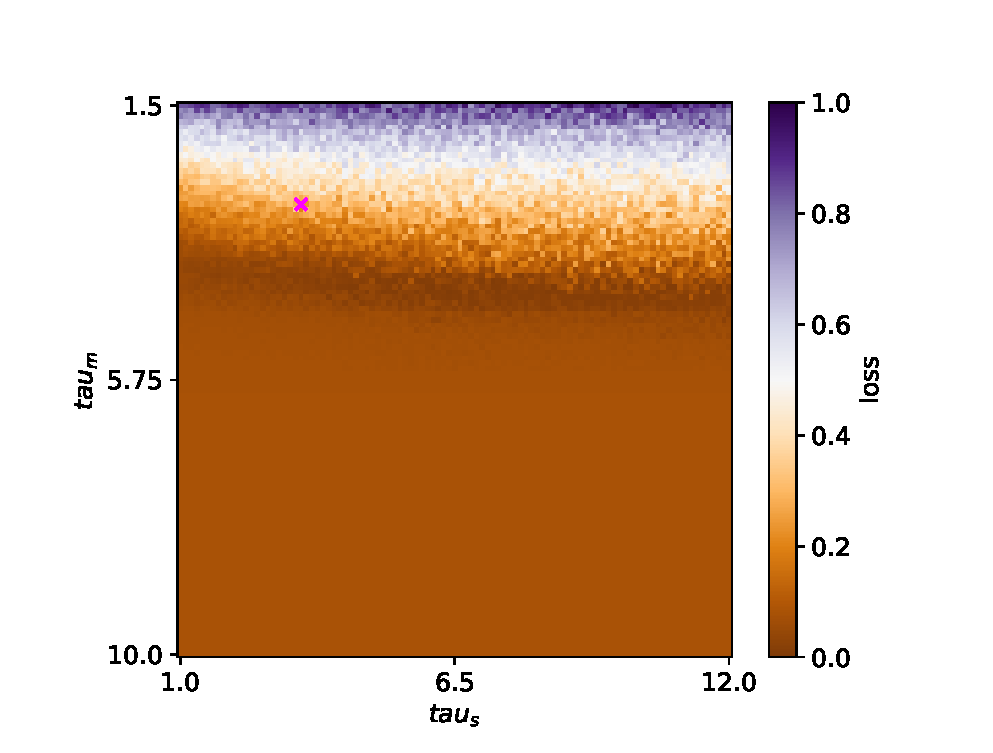
\includegraphics[width=0.7\columnwidth]{figures/param_landscape_heatmaps/GLIF/test_export_2d_heatmap_N_4_loss_tau_s_tau_m.eps}
    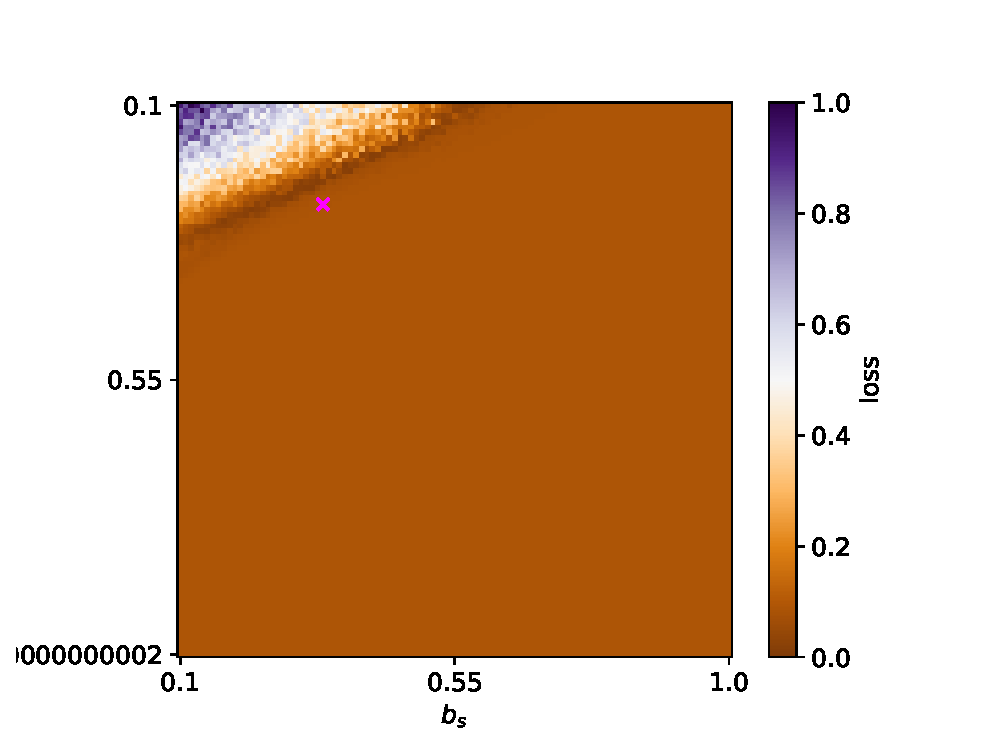
\includegraphics[width=0.7\columnwidth]{figures/param_landscape_heatmaps/GLIF/test_export_2d_heatmap_N_4_loss_b_s_a_v.eps}
    \vskip -0.1in
    \caption{The parameter error landscape for a GLIF SNN for the parameters $\tau_s, \tau_m$ (top), and $b_s, a_v$ (bottom).}
    \label{fig:p_landscape_hmap_GLIF}
\end{figure}


\begin{figure}
    \centering
    \vskip -0.1in
    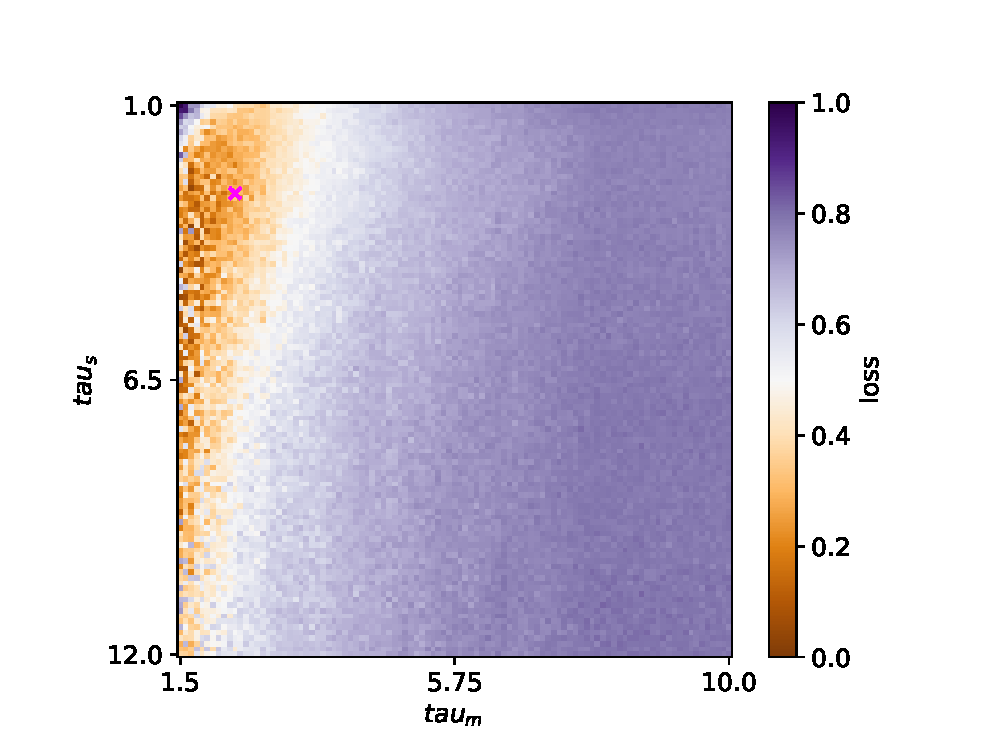
\includegraphics[width=0.7\columnwidth]{figures/param_landscape_heatmaps/LIF/test_export_2d_heatmap_N_4_loss_tau_m_tau_s.eps}
    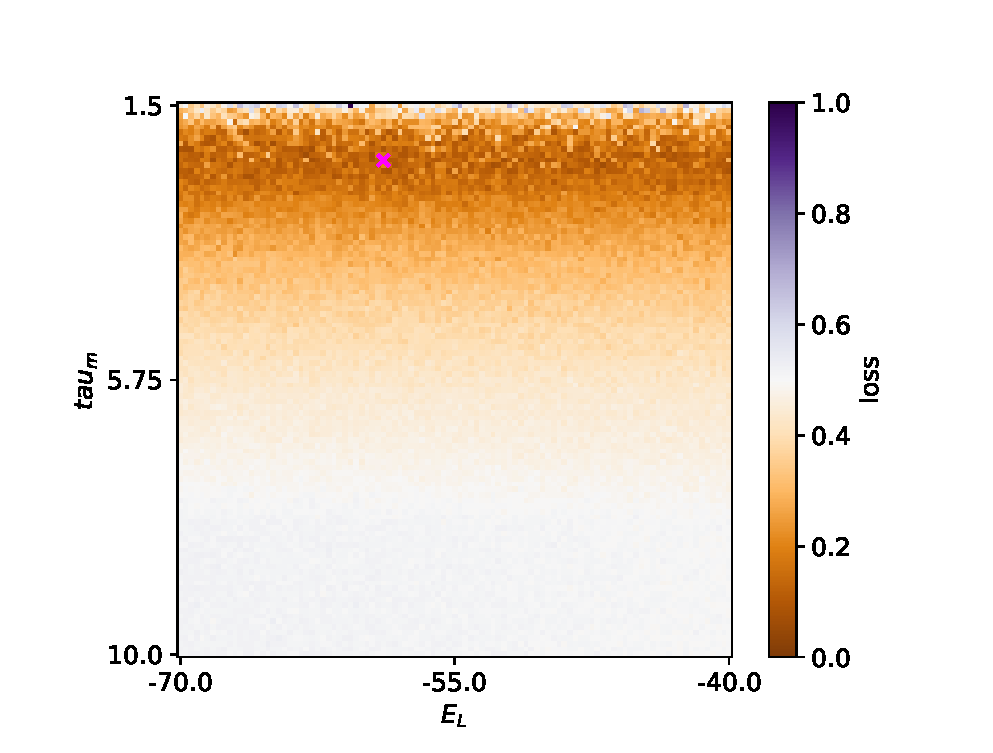
\includegraphics[width=0.7\columnwidth]{figures/param_landscape_heatmaps/LIF/test_export_2d_heatmap_N_4_loss_E_L_tau_m.eps}
    \vskip -0.1in
    \caption{The parameter error landscape for a LIF SNN for the parameters $\tau_s, \tau_m$ (top), and $E_L, \tau_m$ (bottom).}
    \label{fig:p_landscape_hmap_LIF}
\end{figure}


% \subsection{Stochastic integrate-and-fire GBO}

% Bernoulli and Poisson NLL for optimisation.
% Definition outlined in \ref{chpt:background}.

% Population-level GBO for comparison with \cite{Rene2020}.
% Results included below:
% results spike correlations and RMSE, report comparatively too.

% mesoGIF
\begin{figure}
    \centering
    \vskip -0.1in
    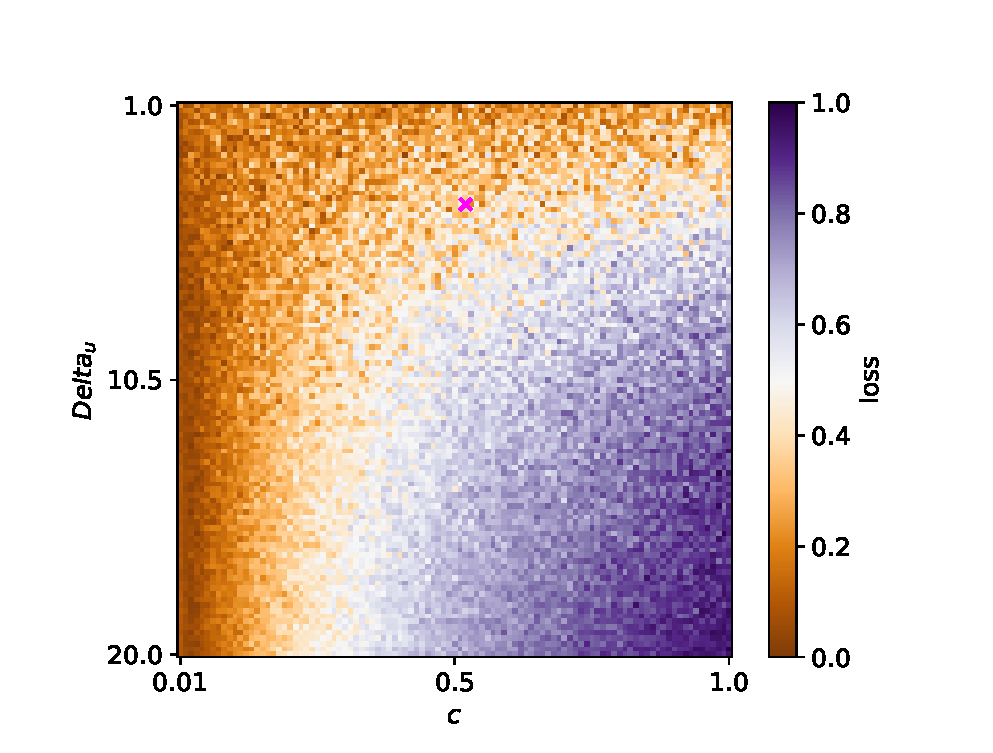
\includegraphics[width=0.7\columnwidth]{figures/param_landscape_heatmaps/microGIF/test_export_2d_heatmap_N_4_loss_c_Delta_u.eps}
    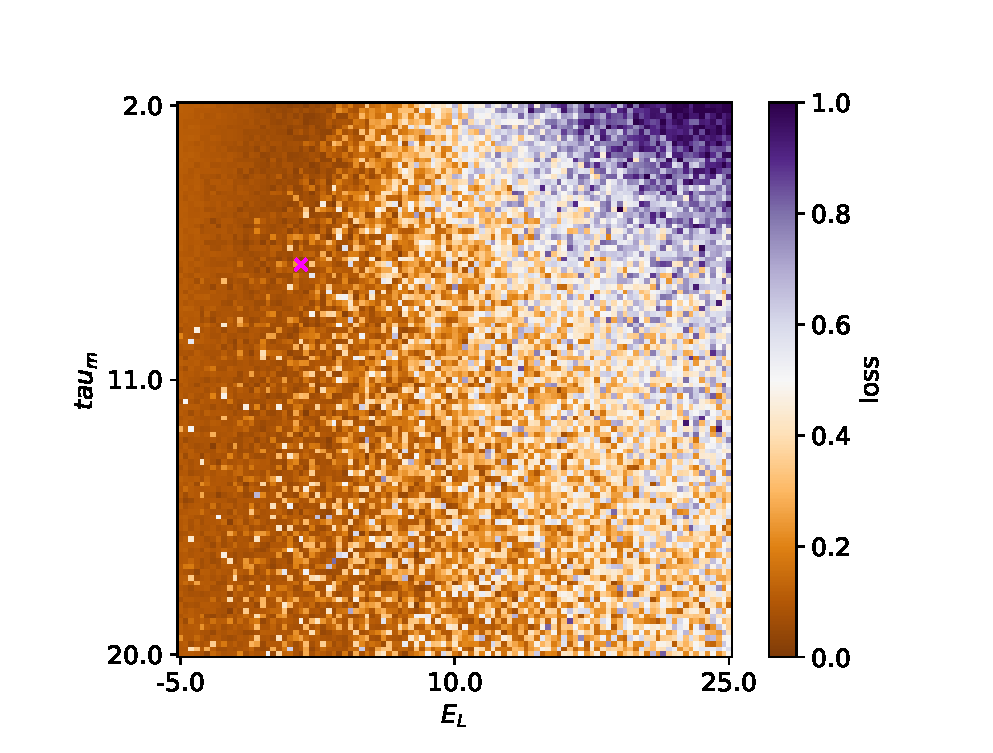
\includegraphics[width=0.7\columnwidth]{figures/param_landscape_heatmaps/microGIF/test_export_2d_heatmap_N_4_loss_E_L_tau_m.eps}
    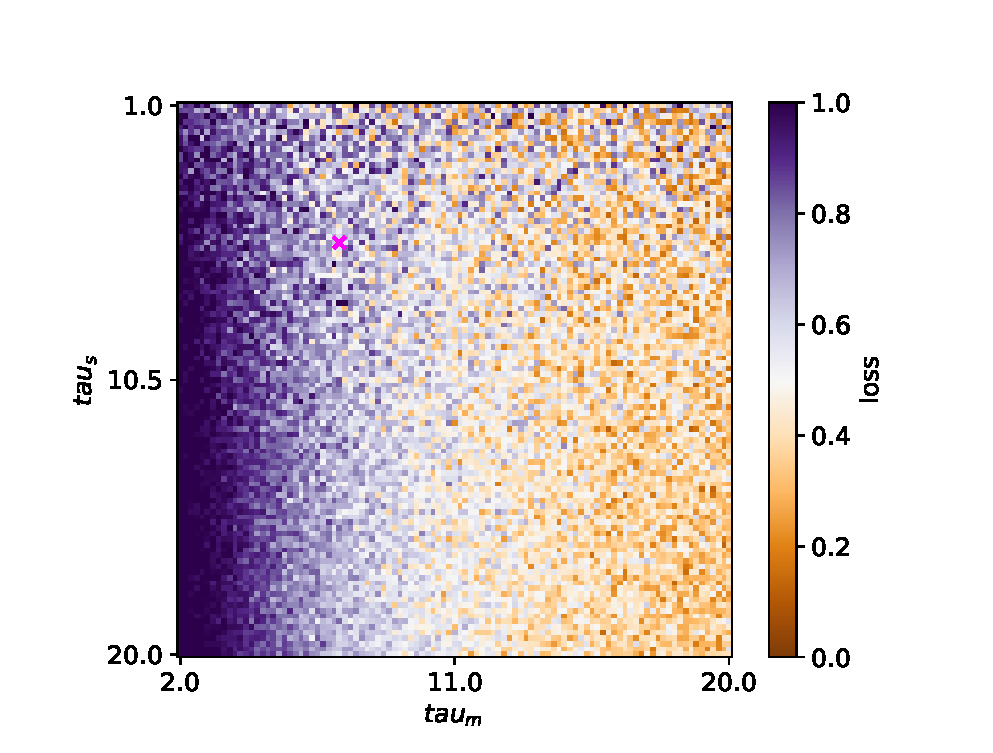
\includegraphics[width=0.7\columnwidth]{figures/param_landscape_heatmaps/microGIF/test_export_2d_heatmap_N_4_loss_tau_m_tau_s.eps}
    \vskip -0.1in
    \caption{The parameter error landscape using the firing rate distance metric, for a population ($N=4$) SGIF model.}
    \label{fig:p_landscape_hmap_SGIF}
\end{figure}


\subsection{Gradient descent with Adam}

To perform optimisation, we used Adam, the adaptive momentum implementation of gradient descent \cite{Kingma2015}.
We note that the spaces for which error gradient given by the firing rate distance is ambiguous, i.e. the gradient may wander somewhat arbitrarily into the space of low to zero error, where it settles, and is thus not satisfactory in terms of defining a signal that will allow for retrieving the ground-truth.
Further, for the van Rossum distance, these landscapes are even more obscure and noisy. Therefore, we have excluded using this metric in our experiments in this work.
However, under more well-defined conditions, where the timing of individual spikes relative to the input signal and other neurons' signals is more informative than misleading, the van Rossum distance should theoretically outperform the firing rate distance.
% ... (plot generation if time)

For each model type, we used the firing rate distance from the target synthetic model outputs to the model being fitted, to optimise its parameters, as previously mentioned until the error gradients were diminishing and thus parameters settling into a local minimum, or for a certain number of training iterations ($t_{iter}=100$.
This was performed for $20$ experiments, for each model class. We then assess the fitted model rates, parameter values, and the loss, and perform NMF analysis on fitted model as well as target model and data, assessing the geodesic similarity of the factorised modules.
% This gives us 

Further, we perform direct neuron-level, i.e. full-scale, model inference of a heterogeneous mixture of stochastic general integrate-and-fire (SGIF) neurons, and find that albeit converging to local minima, the stochastic formulation and the optimisation over the NLL lends itself better to GBO than the surrogate over the LIF-model types when using the firing rate distance.
For all model classes, some parameters have a more prominent effect on the the loss than others, particularly when considering the rate-based loss metric. 
% This is in part handled by using Adam. 
% When considering the NLL, the parameter landscape plots reveal that 
% Illuminating ...


\section{Results}

Results are reported for 20 experiments for each model class, fitted to models of size $N=4$ for LIF and GLIF neurons in this chapter, and synthetically for SGIF models to models of size $N=4$ as well as $N=21$.
These are abbreviated as "meGIF" and "miGIF" respectively - representing meso-GIF and micro-GIF, adopted from \cite{Rene2020}.
The main results are the rates per configuration (i.e. model class and loss function) - implicitly also representing the loss, the parameter distances from the fitted to the ground-truth models, and the geodesic similarities as obtained via NMF.

\subsection{GBO results}

% \begin{figure}
%     \centering
%     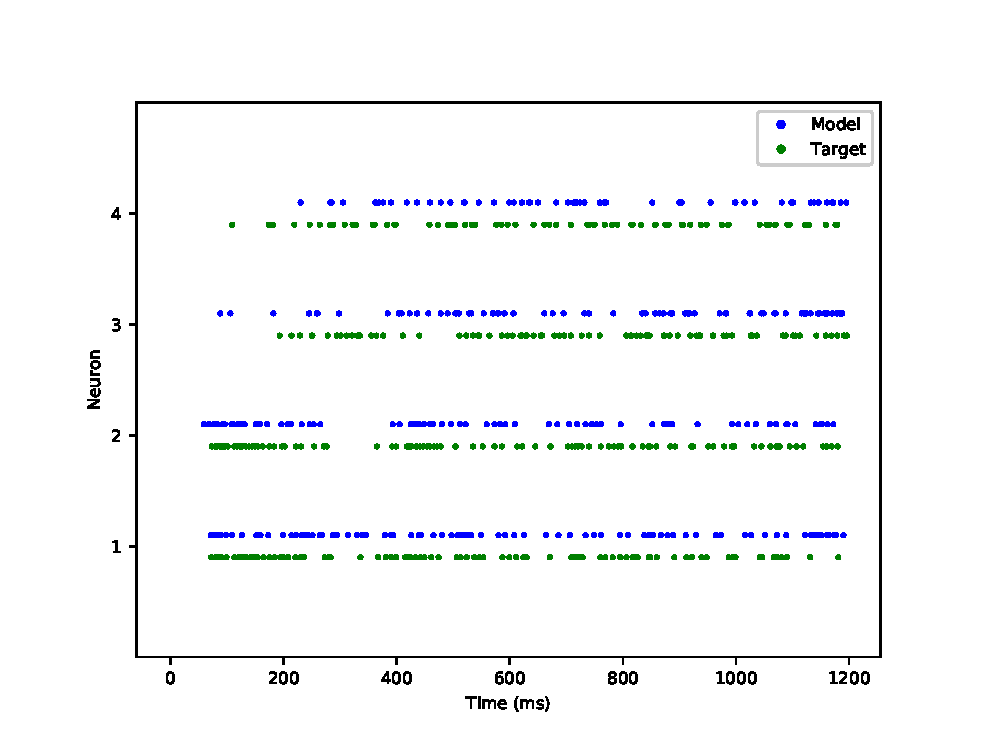
\includegraphics[width=0.4\columnwidth]{figures/samples/SameModelClassTarget/export_spike_trains_euid_12-09_16-17-13-464.eps}
%     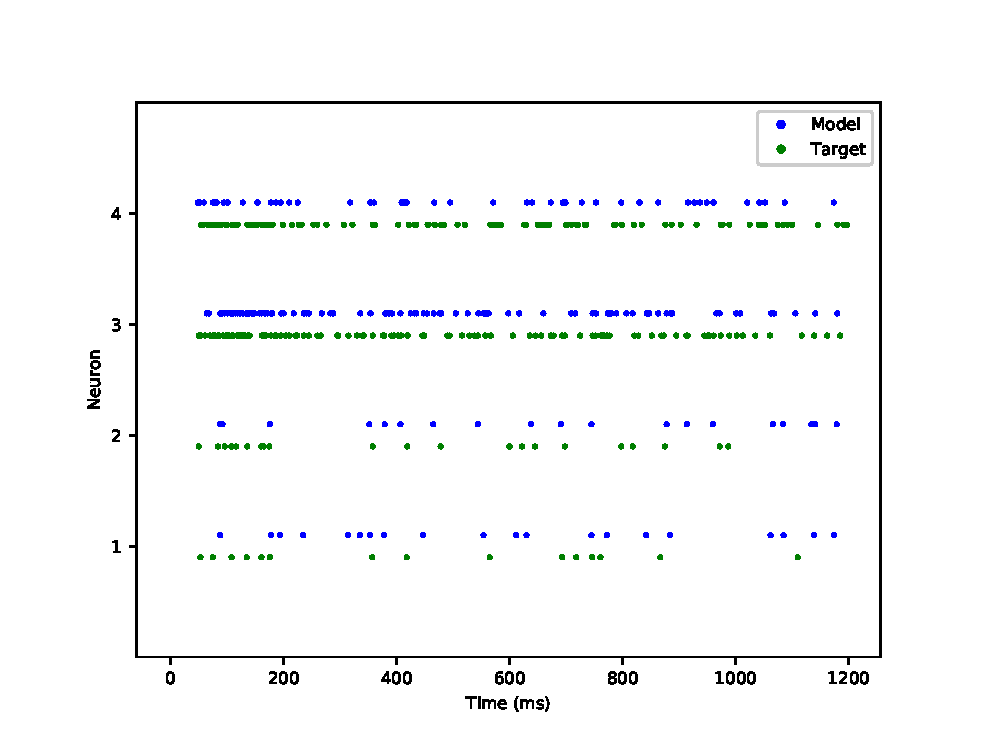
\includegraphics[width=0.4\columnwidth]{figures/samples/SameModelClassTarget/export_spike_trains_euid_12-10_09-45-02-423.eps}
%     \caption{Sample LIF and GLIF SNNs after fitting, N=4.}
%     \label{fig:sample_LIF_GLIF_N_4}
% \end{figure}

Included here are figures from two experiments, one for a GLIF SNN, and one for a LIF SNN, illustrated in figures \ref{fig:sample_GLIF_exp}, \ref{fig:sample_GLIF_exp_vs_traject}, \ref{fig:sample_LIF_exp_spikes_loss}, \ref{fig:sample_LIF_exp_vs_traject}.
As may be glimpsed from these, particularly for the LIF model, we may end up in local minima further away from the ground truth. On average, we end up further from the ground truth for LIF models, and around the same distance for GLIF models, whereas for SGIF models, we end up somewhat closer.
As for the rates, these also reflect these results, with the closes fits being attained for the GLIF and SGIF models.

\begin{figure}
    \centering
    \vspace{-0.1in}
    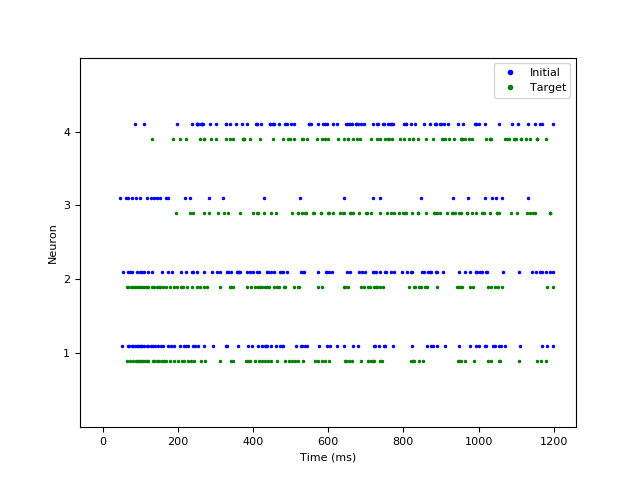
\includegraphics[width=0.9\linewidth]{figures/samples/GLIF/12-09_16-14-54-627/spike_trains_train_iter_100.png}
    \vspace{-0.1in}
    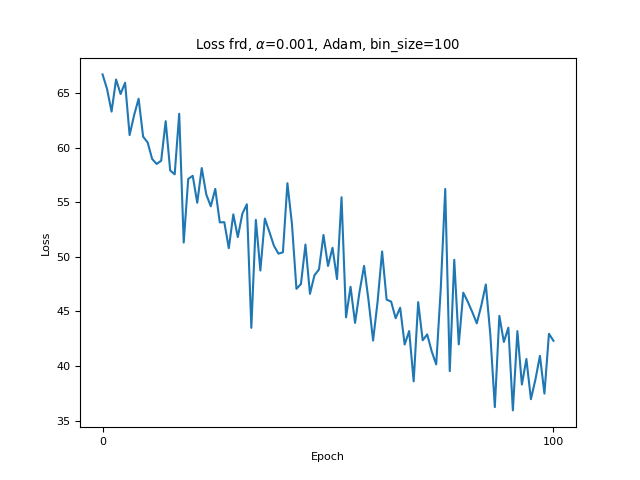
\includegraphics[width=0.9\linewidth]{figures/samples/GLIF/12-09_16-14-54-627/plot_loss_test12-09_16-16-45-54312-09_16-16-45-543.png}
    \vspace{-0.1in}
    \caption{Sample GLIF SNN, spike trains after training (top) for a particular experiment, along with the loss per epoch (bottom), corresponding membrane potentials and parameter inference trajectories in \ref{fig:sample_GLIF_exp_vs_traject}.}
    \label{fig:sample_GLIF_exp}
\end{figure}

\begin{figure}
    \centering
    \vspace{-0.1in}
    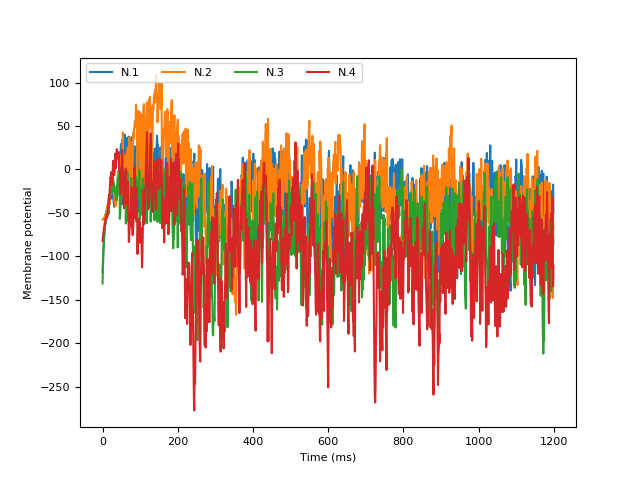
\includegraphics[width=0.9\linewidth]{figures/samples/GLIF/12-09_16-14-54-627/membrane_pots_train_i_100.png}
    \vspace{-0.1in}
    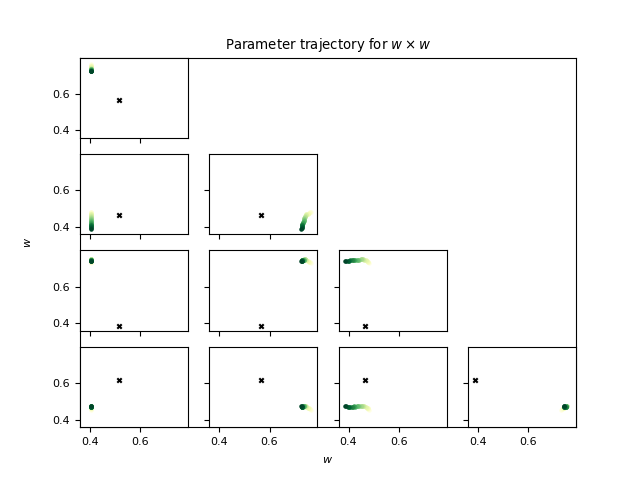
\includegraphics[width=0.9\linewidth]{figures/samples/GLIF/12-09_16-14-54-627/test_weights_inference_trajectories_param_w.png}
    \vspace{-0.1in}
    \caption{Membrane potentials (top) for the spike train plotted in \ref{fig:sample_GLIF_exp}, and the average trajectory (bottom) of the weights throughout inference.}
    \label{fig:sample_GLIF_exp_vs_traject}
\end{figure}

\begin{figure}
    \centering
    \vspace{-0.1in}
    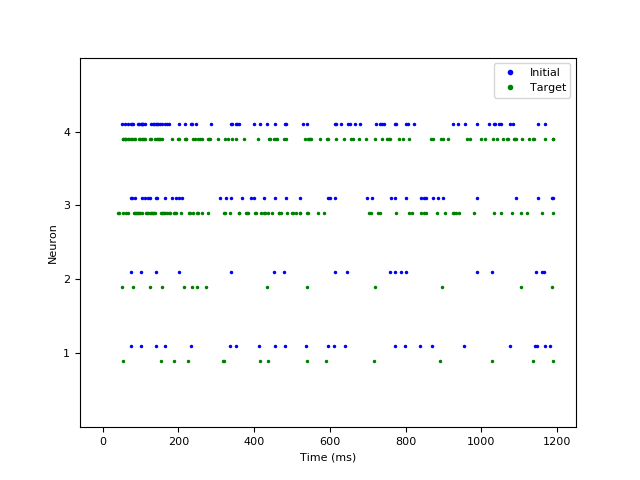
\includegraphics[width=0.9\columnwidth]{figures/samples/LIF/12-10_09-55-57-223/spike_trains_train_iter_100.png}
    \vspace{-0.1in}
    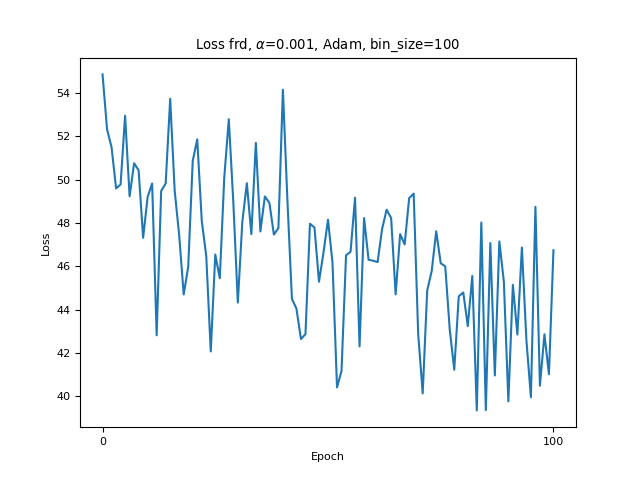
\includegraphics[width=0.9\columnwidth]{figures/samples/LIF/12-10_09-55-57-223/plot_loss_test12-10_09-56-55-12812-10_09-56-55-128.png}
    \vspace{-0.1in}
    \caption{Sample LIF SNN, spike trains after training for a particular experiment, along with the loss per epoch, and corresponding membrane potentials for the spike train plotted above and the average trajectory of the weights throughout inference in \ref{fig:sample_GLIF_exp_vs_traject}.}
    \label{fig:sample_LIF_exp_spikes_loss}
\end{figure}

\begin{figure}
    \centering
    \vspace{-0.1in}
    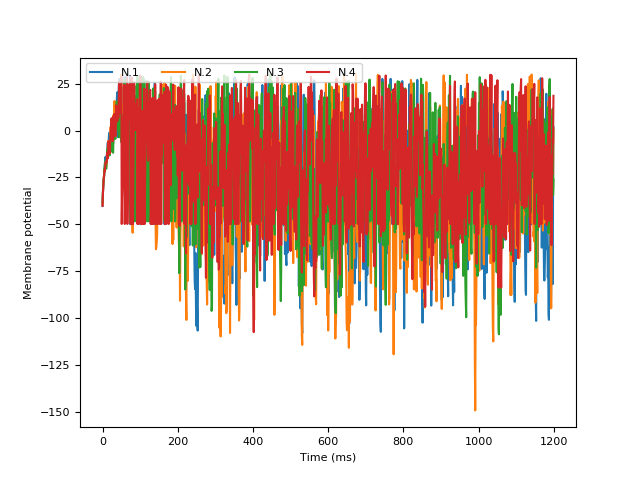
\includegraphics[width=0.9\columnwidth]{figures/samples/LIF/12-10_09-55-57-223/membrane_pots_train_i_100.png}
    \vspace{-0.1in}
    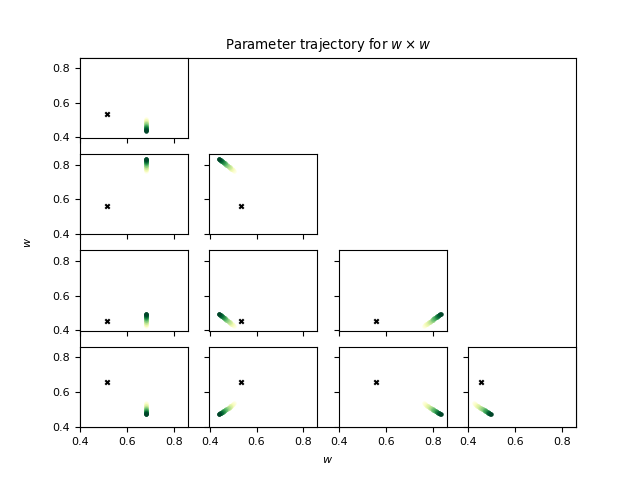
\includegraphics[width=0.9\columnwidth]{figures/samples/LIF/12-10_09-55-57-223/test_weights_inference_trajectories_param_w.png}
    \vspace{-0.1in}
    \caption{Sample LIF SNN membrane potentials for the spike train plotted in \ref{fig:sample_LIF_exp_spikes_loss}, and the average trajectory of the weights throughout inference.}
    \label{fig:sample_LIF_exp_vs_traject}
\end{figure}

% \subsubsection{Average model rate and parameter distance}

% GBO
\begin{figure}
    \centering
    \vspace{-0.1in}
	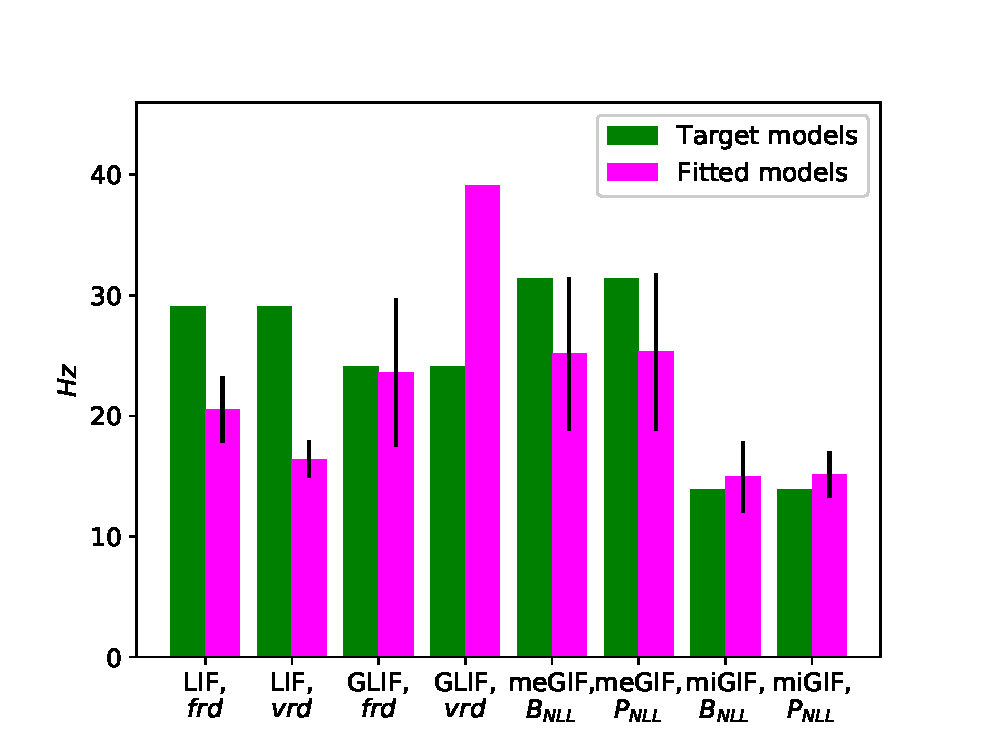
\includegraphics[width=0.8\columnwidth]{figures/export_rates_saved_all.eps}
	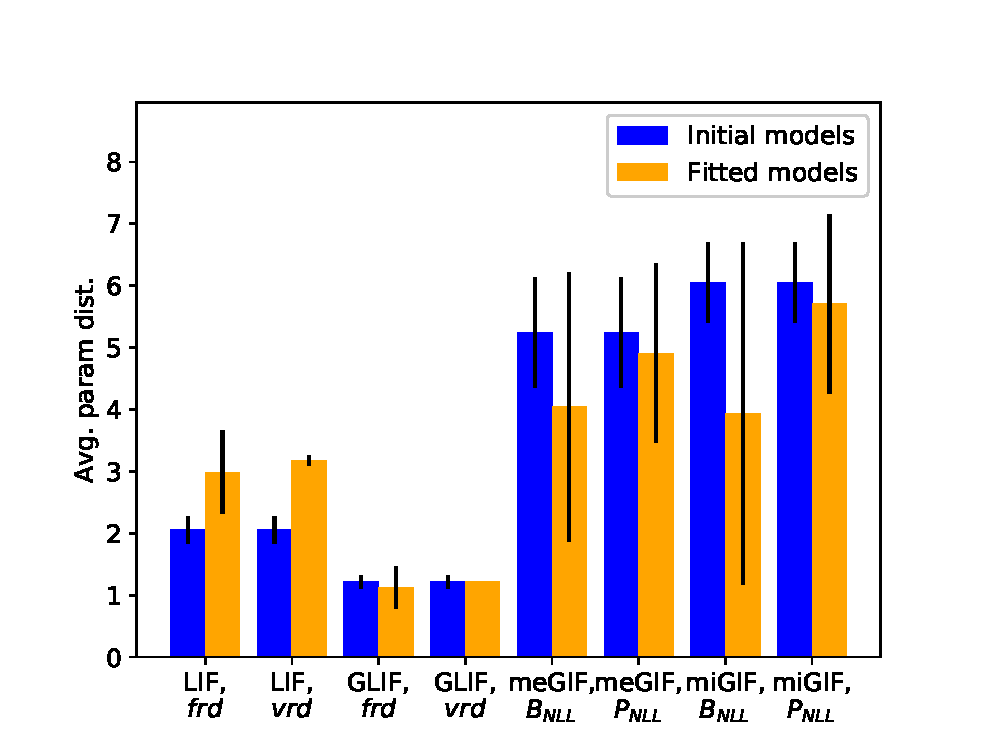
\includegraphics[width=0.8\columnwidth]{figures/export_p_dists_saved_all.eps}
	\vspace{-0.1in}
	\caption{Fitted model rates across model types and loss metrics, and average parameter distance between the ground-truth model and both the initial and converged inferred models when using \textbf{GBO} for model inference. See figure \ref{fig:rate_p_dists_SBI} for comparison with SBI.}
	\label{fig:rate_p_dists_GBO}
\end{figure}

Overall, these results, particularly illustrated by the average parameter distances in figure \ref{fig:rate_p_dists_GBO}, show that ground-truth retrieval is highly unlikely with the specified model definitions and loss metrics, as illuminated by the error landscape plots in \ref{sect:e_landscapes}.

\clearpage
\subsection{Stochastic general integrate-and-fire neurons}

\begin{figure}
    \centering
    \vspace{-0.1in}
    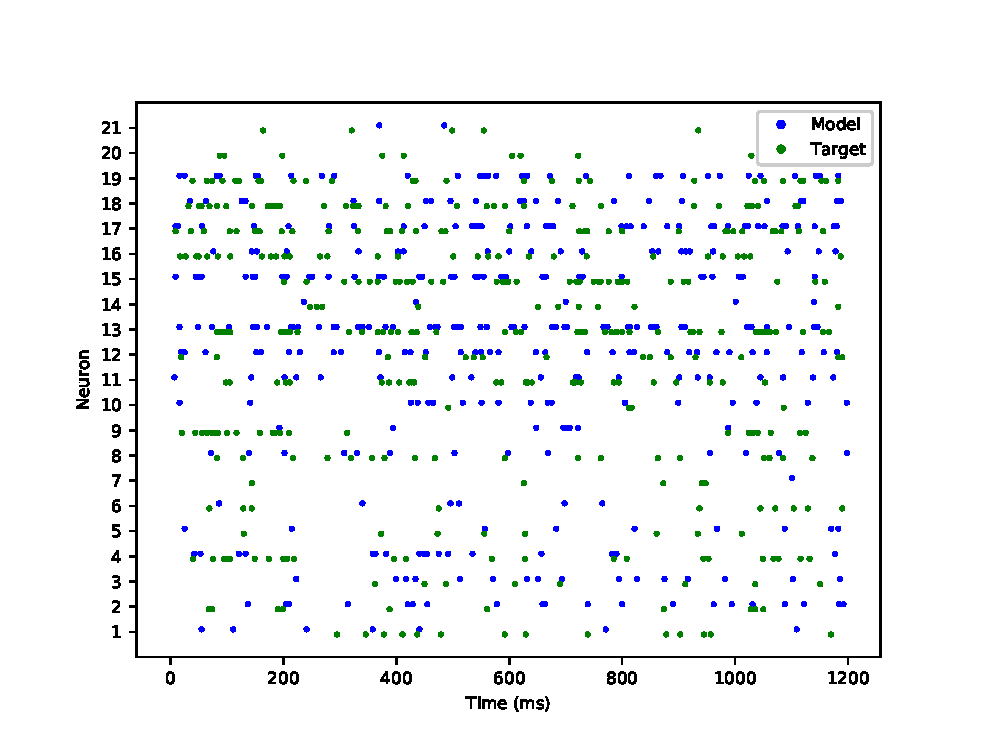
\includegraphics[width=0.9\columnwidth]{figures/samples/SameModelClassTarget/poisson/12-09_17-56-51-235/export_spike_trains_euid_12-09_17-56-51-235.eps}
    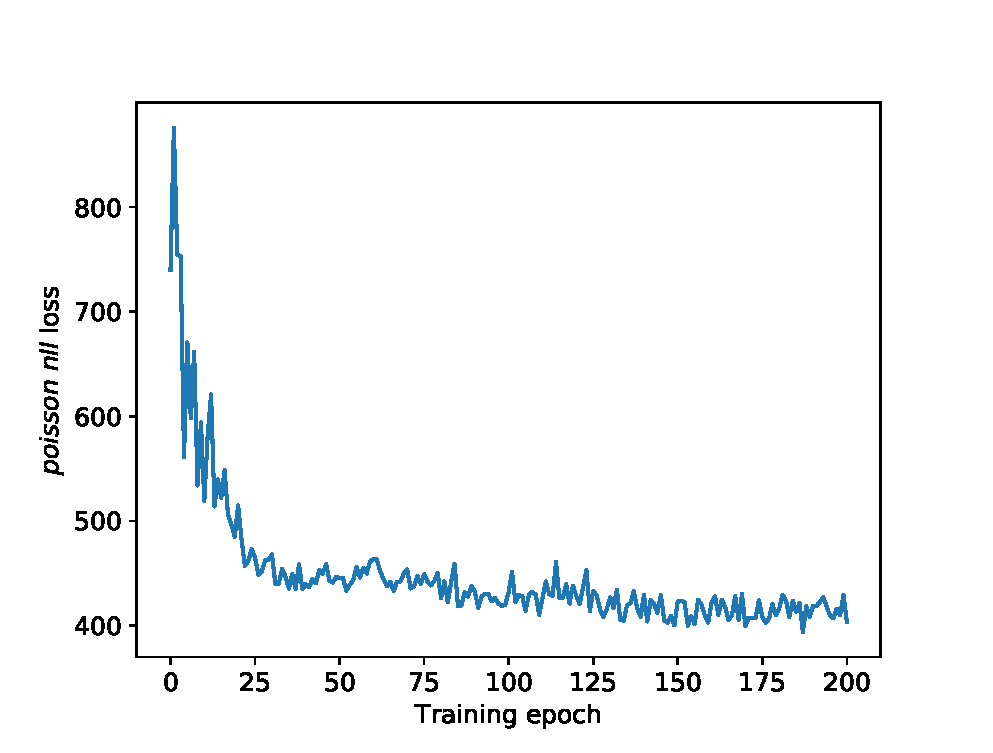
\includegraphics[width=0.7\columnwidth]{figures/samples/SameModelClassTarget/poisson/12-09_17-56-51-235/export_microGIF_plot_loss_euid_12-09_17-56-51-235.eps}
    \vspace{-0.1in}
    \caption{Target and fitted SGIF model spike trains, and loss per training epoch, with the Poisson negative log-likelihood as the loss metric (bottom).}
    \label{fig:sample_SGIF_plots}
\end{figure}

% \begin{figure}
%     \centering
    
%     \caption{The Poisson negative log-likelihood loss per epoch for the experiment with the spike train after training plotted in figure \ref{fig:sample_SGIF_plots}.}
%     \label{fig:PNLL_SGIF_sample_loss}
% \end{figure}

Figure \ref{fig:sample_SGIF_plots} illustrates that GBO is possible for direct, scalable inference of neuron-level models when using a stochastic formulation of the LIF model and the Bernoulli or Poisson NLL by assuming spikes distributed in either of the corresponding probability densities, both being exponential family distributions with shared properties for the case of spike trains.
However, as is found and described in table \ref{tab:rho_converged_GBO_pop}, the models are less correlated than when using MCMC sampling over the full posterior.
It can be argued that this is expected, since no parameter dependence is assumed in the GBO inference methodology, as in the ABC-procedure of \cite{Rene2020}.
Convergence rates are nonetheless good (table \ref{tab:rmse_converged_GBO_pop}), and parameter distances are somewhat closer on average when using GBO (figure \ref{fig:rate_p_dists_GBO}), and in contrast significantly further away from the ground-truth than the initial, pseudorandomly distributed model parameters in the case of SBI (see figure \ref{fig:rate_p_dists_SBI}).

% SameModelClassTarget
% \subsection{Known ground-truth synthetic data}


\subsubsection{Comparison with published ABC results}

In addition to implementation of GBO for LIF and GLIF SNNs, we test our approach on SGIF neurons, which may lend themselves better to GBO with NLL minimisation over spike probabilities. We here report our comparative results for this model class, as when compared to the work which we adopted the model from \cite{Rene2020}.

\subsubsection{Model input perturbation and formulation}

While we want to model the site from which spikes have been recorded and decoded, we do not have the input to the site recorded from in biological spike train data, as is often the case.
However, we may make some assumptions about the statistical nature of the input data, and incorporate this into model perturbation. Optionally, we may even design a particular perturbation scheme, such as sinusoidal stimulation, as this may also be performed in vitro.
In this work we perturb the models with white noise for the rate-based experiments, sine-modulated white noise during training, and also with an Ornstein-Uhlenbeck process during testing of the stochastic general integrate-and-fire (SGIF) models (also optimising over the NLL as previously mentioned) as done in \cite{Rene2020} in order to keep our methods as consistent as possible and therefore results more comparable by adopting and extending their work, and lastly with sine-modulated linear transformations using different random seeds for our implementation and extension of \cite{Huh2018} where we similarly adopt their procedure.

% In the SGIF model, we assume that the model activity and spike history can be expressed as a set of stochastic equations, which then allows us to optimise over the model spike probabilities for given target spike histories.
% In order to test GBO for the SGIF model class, and for comparability with \cite{Rene2020}, we adopt their perturbation scheme, and perturb our models with both sine modulated white noise, and with by using an Ornstein-Uhlenbeck process, and report the results for each case.

% \subsubsection*{Sine modulated white noise input}

% \begin{equation}
%     \sum^M \sin(W_n(t))
% \end{equation}

% \subsubsection*{White noise input}

% \begin{equation}
%     W_n(t) \sim \mathcal{U}(t, m)
% \end{equation}


\begin{table}
\caption{Neuronal correlations $\rho$ for GBO, converged runs, network size N=4, for the SGIF SNN.}
\label{tab:rho_converged_GBO_pop}
\begin{center}
\begin{tabular}{ l l c c c c c }
 & & \multicolumn{4}{c}{$\rho$ per neuron} \\
 & & $e_{L2/3}$ & $i_{L2/3}$ & $e_{L4}$ & $i_{L4}$ \\
 \textbf{WN} & \textbf{Bernoulli} & 0.09 & 0.14 & 0.21 & 0.07 \\ 
 \textbf{WN} & \textbf{Poisson} & 0.27 & -0.02 & -0.02 & 0.04 \\  
 \textbf{OU} & \textbf{Bernoulli} & 0.23 & 0.35 & 0.14 & 0.14 \\ 
 \textbf{OU} & \textbf{Poisson} & 0.22 & -0.03 & 0.04 & 0.03 \\  
\end{tabular}
\end{center}
\end{table}

\begin{table}
\caption{RMSE for GBO, converged runs, network size N=4, for the SGIF SNN.}
\label{tab:rmse_converged_GBO_pop}
\begin{center}
\begin{tabular}{ l l c c c c c c }
& & \multicolumn{4}{c}{RMSE per neuron} & \textit{Convergence} \\
& & $e_{L2/3}$ & $i_{L2/3}$ & $e_{L4}$ & $i_{L4}$ \\
 \textbf{WN} & \textbf{Bernoulli} & 8.9 & 11.5 & 19.9 & 29.0 & 50 \% \\ 
 \textbf{WN} & \textbf{Poisson} & 11.5 & 14.6 & 19.8 & 25.0 & 80 \% \\  
 \textbf{OU} & \textbf{Bernoulli} & 8.7 & 10.8 & 16.8 & 28.6 & 70 \% \\ 
 \textbf{OU} & \textbf{Poisson} & 11.2 & 13.3 & 17.3 & 25.5 & 85 \% \\  
\end{tabular}
\end{center}
\end{table}

For further results on this model class, including the geodesic NMF module similarity, this is included outwith this subsection, alongside the results for the other model classes.



\subsection{Simulation-based inference}

Using the best performing loss-metric as found in the GBO experiments, and also revealed by the parameter landscape plots, i.e. the firing rate loss metric, we performed SBI by using the Python-framework of the Macke-lab \href{https://github.com/mackelab/sbi}{SBI}.

In sum, SBI over a rate-based metric performed slightly worse for SGIF, and for the leaky integrate-and-fire models was on par for the less high-dimensional LIF model, but performed worse for the more complex GLIF model.
As for retrieving the ground truth parameters, this is where SBI might supplement and/or outperform a GBO approach, as we calculate the full posterior over the model parameters, given the observations.
Interestingly, however, even for the relatively low-dimensional LIF-model, the posteriors are somewhat skewed to the side of the ground-truth values. They do indeed generally give a reasonable estimate for the centers of the pdfs for the parameters for the LIF model, and to some extent for the SGIF model, but fails to do so for the GLIF model.
The declining performance matches well with the increasing number of model parameters, which might be expected with an ABC approach, as posterior approximation requires increasingly more patterns with an increasing dimensionality - and likely even exponentially so.
This shows that particularly for more complex models, which SNNs quite often are, the advantages and applicability of ABC may diminish - rendering GBO if not the only tractable approach, even a competitive wrt parameter inference.

\begin{figure}
    \centering
    \vspace{-0.2in}
	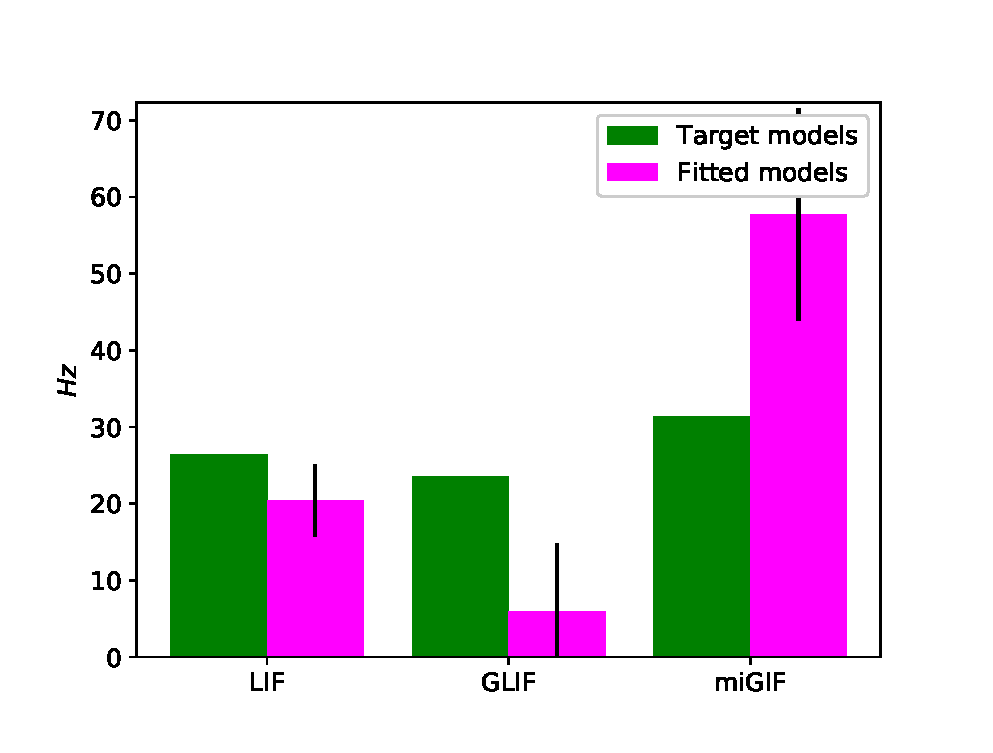
\includegraphics[width=0.7\columnwidth]{figures/sbi_plot_rates_all.eps}
	\vspace{-0.1in}
	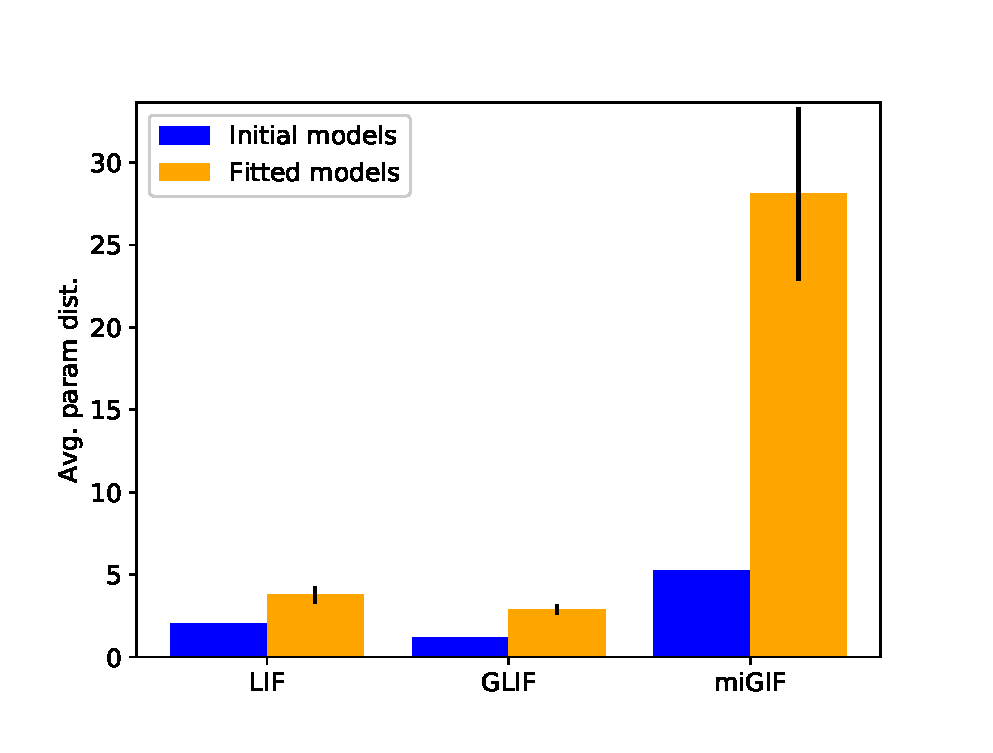
\includegraphics[width=0.7\columnwidth]{figures/sbi_mean_p_dist_all.eps}
	\vspace{-0.1in}
	\caption{Fitted model rates across model types and loss metrics, and average parameter distance between the ground-truth model and both the initial and converged inferred models when using \textbf{SBI} for model inference. See figure \ref{fig:rate_p_dists_GBO} for comparison with GBO.}
	\label{fig:rate_p_dists_SBI}
\end{figure}


\begin{figure}
    \centering
	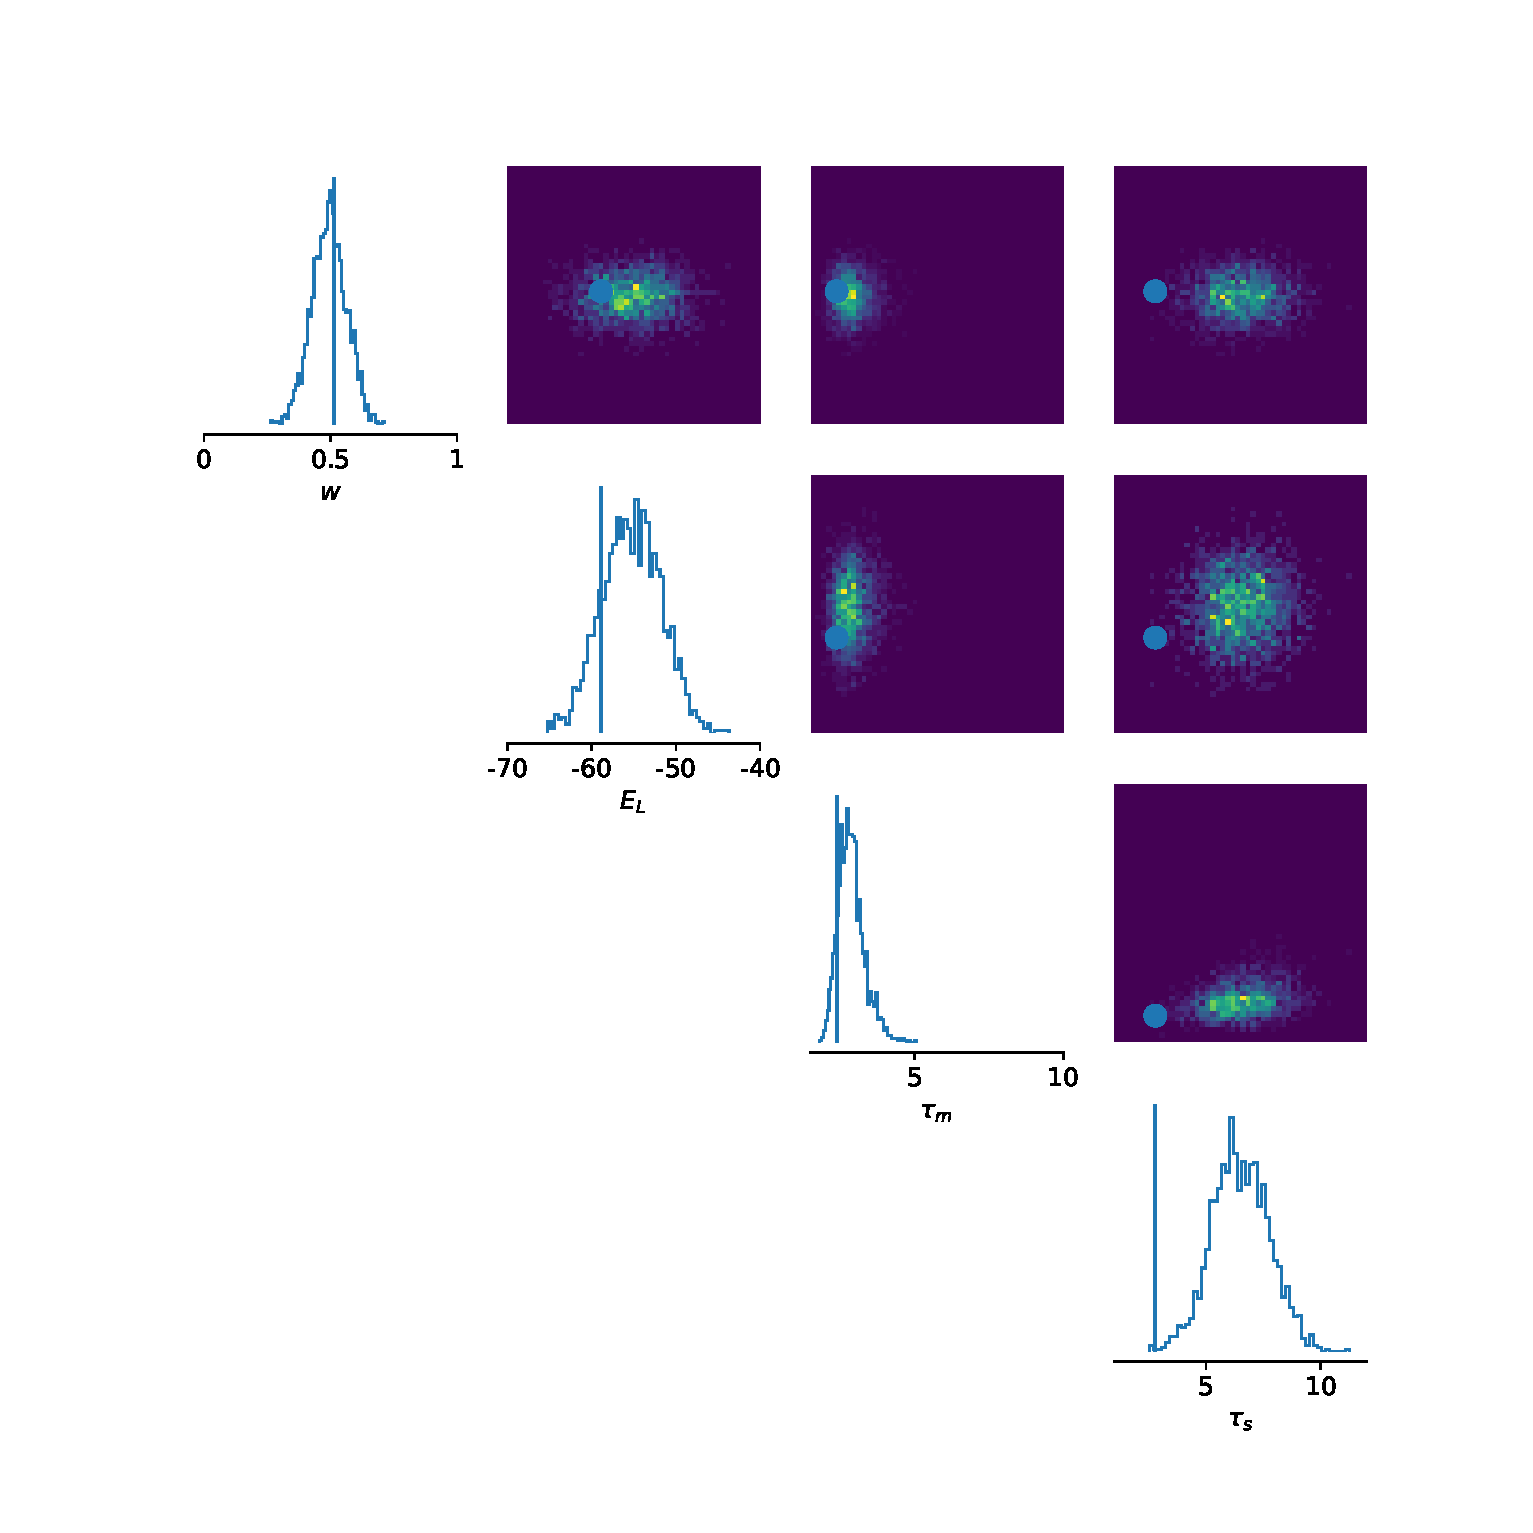
\includegraphics[width=0.9\columnwidth]{figures/sbi_p_avgs_pairplot_SNPE_LIF_12-15_04-56-19-338.eps}
	\caption{Mean posterior marginals between parameters for the LIF model class, fitted using the same ground-truth model and synthetic data as in the LIF GBO experiments.}
	\label{fig:mean_posterior_marginal_SNPE_LIF}
\end{figure}

\begin{figure}
    \centering
	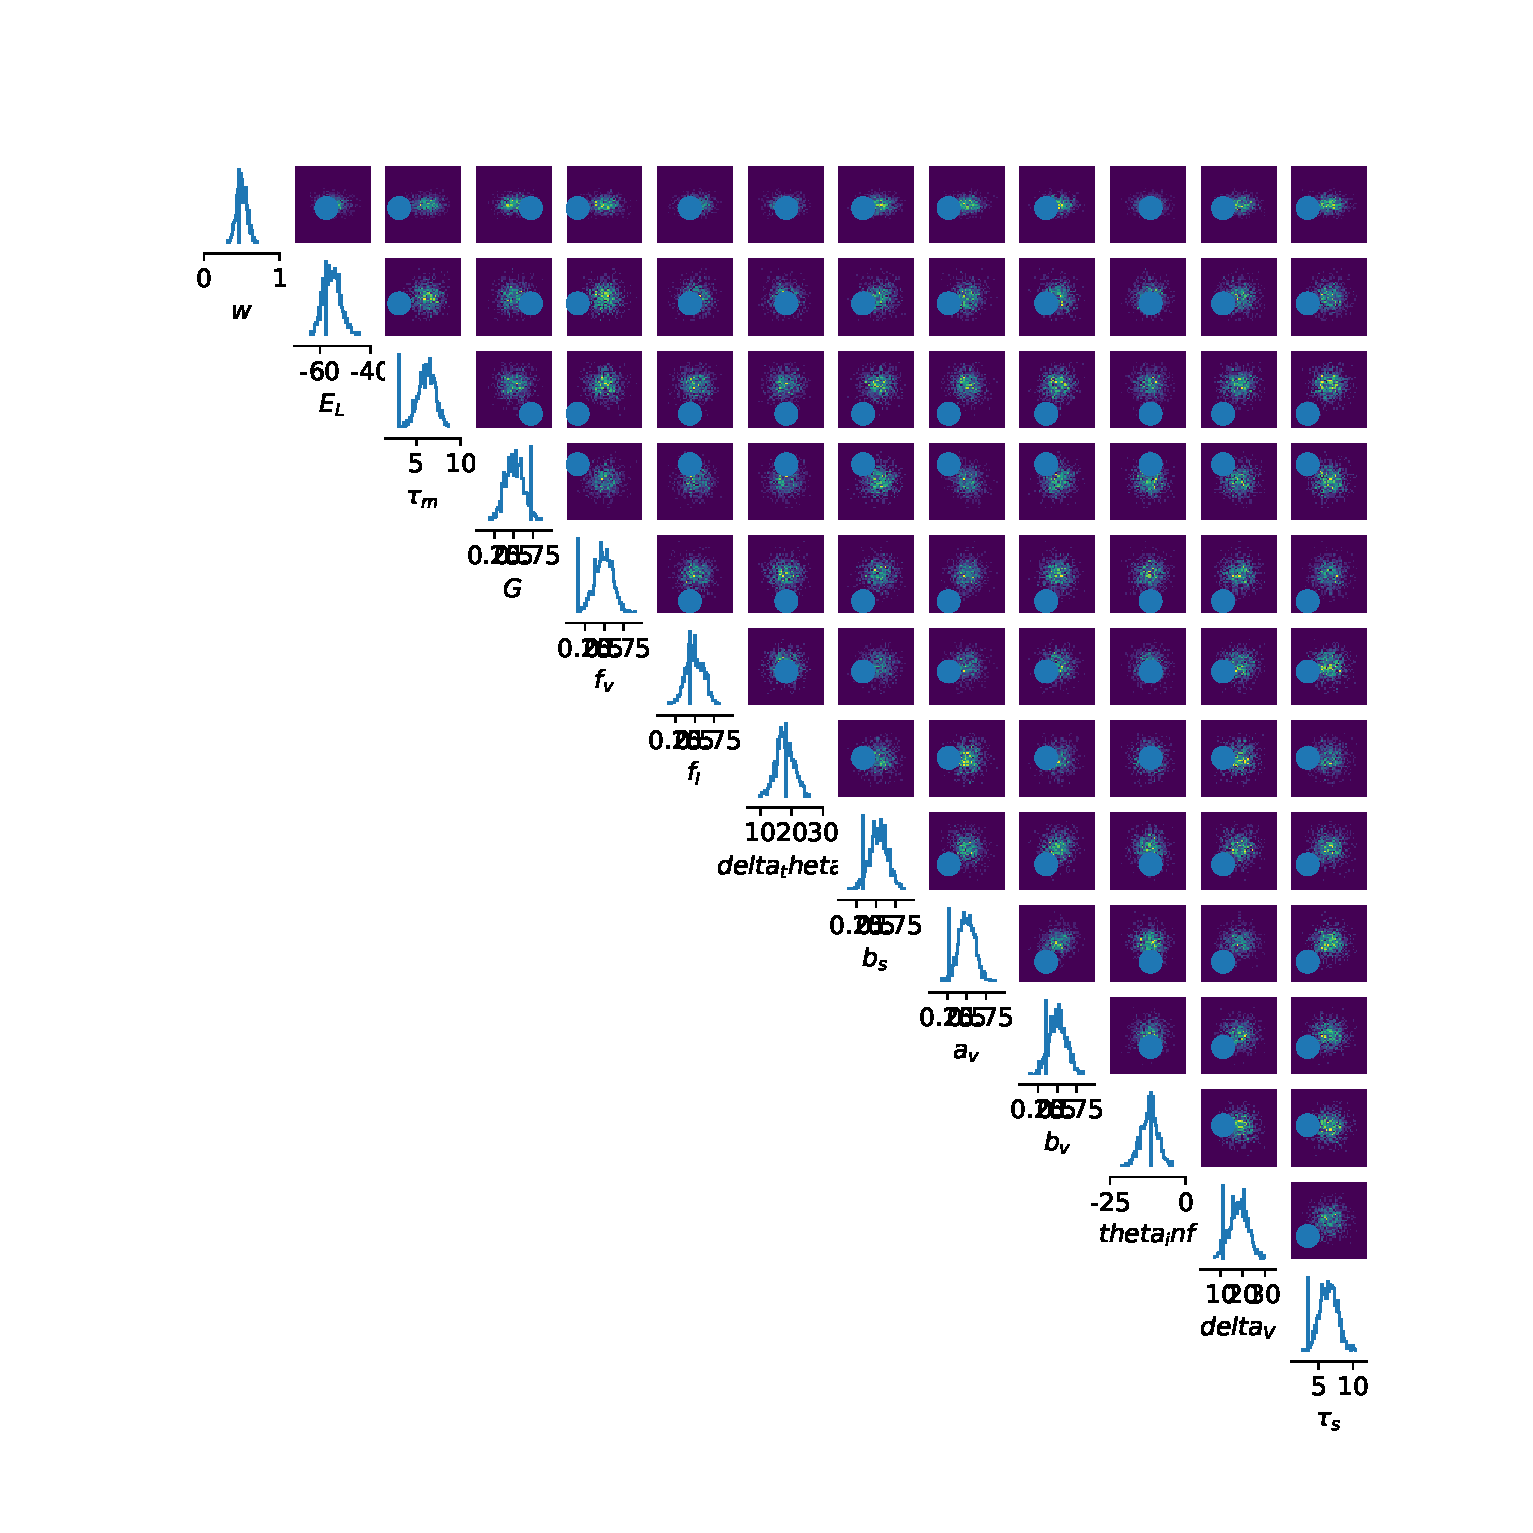
\includegraphics[width=\columnwidth]{figures/sbi_p_avgs_pairplot_SNPE_GLIF_12-15_14-22-38-919.eps}
	\caption{Mean posterior marginals between parameters for the GLIF model class.}
	\label{fig:mean_posterior_marginal_SNPE_GLIF}
\end{figure}

\begin{figure}
    \centering
	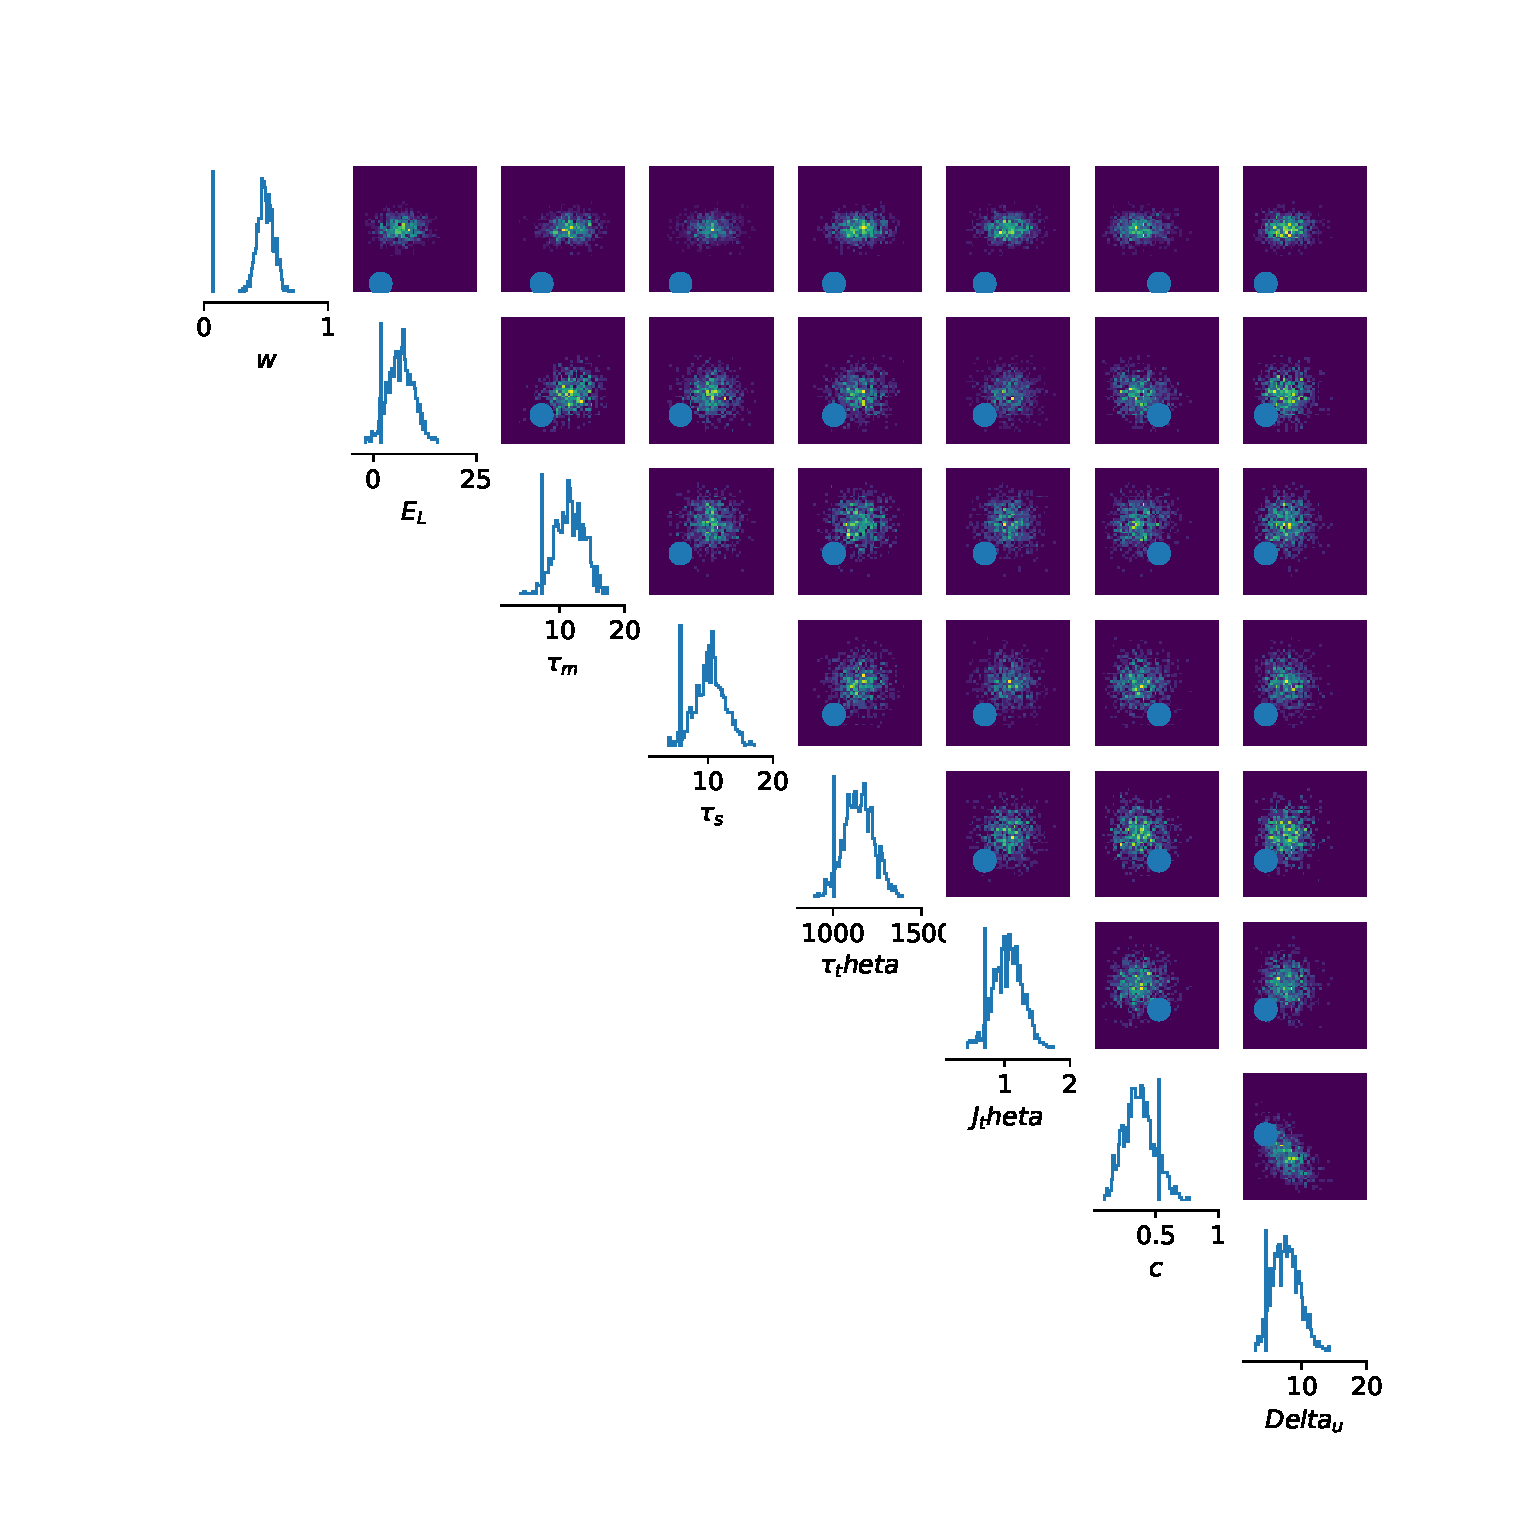
\includegraphics[width=\columnwidth]{figures/sbi_p_avgs_pairplot_SNPE_microGIF_12-14_16-14-12-736.eps}
	\caption{Mean posterior marginals between parameters for the SGIF model class.}
	\label{fig:mean_posterior_marginal_SNPE_SGIF}
\end{figure}


\clearpage
\subsection{NMF analysis}

We analyse the fits attained with the different approaches in order to assess to what extent the inferred models capture functional organisation of the networks that generated the target data.
A high similarity of the factorised representations of neuronal co-activity indicates that the inferred models capture the spatiotemporal behaviour of the target model, which may suggest that the model can be used for further evaluation, such as ing probing to assess functional aspects or in testing or generating functionally related hypotheses. These are more relevant for biological data sets, of course.



% Custom coupled GLM fitted to target spike trains. Baseline.
% citecite

% \begin{figure}
%     \hspace{-0.1\columnwidth}
%     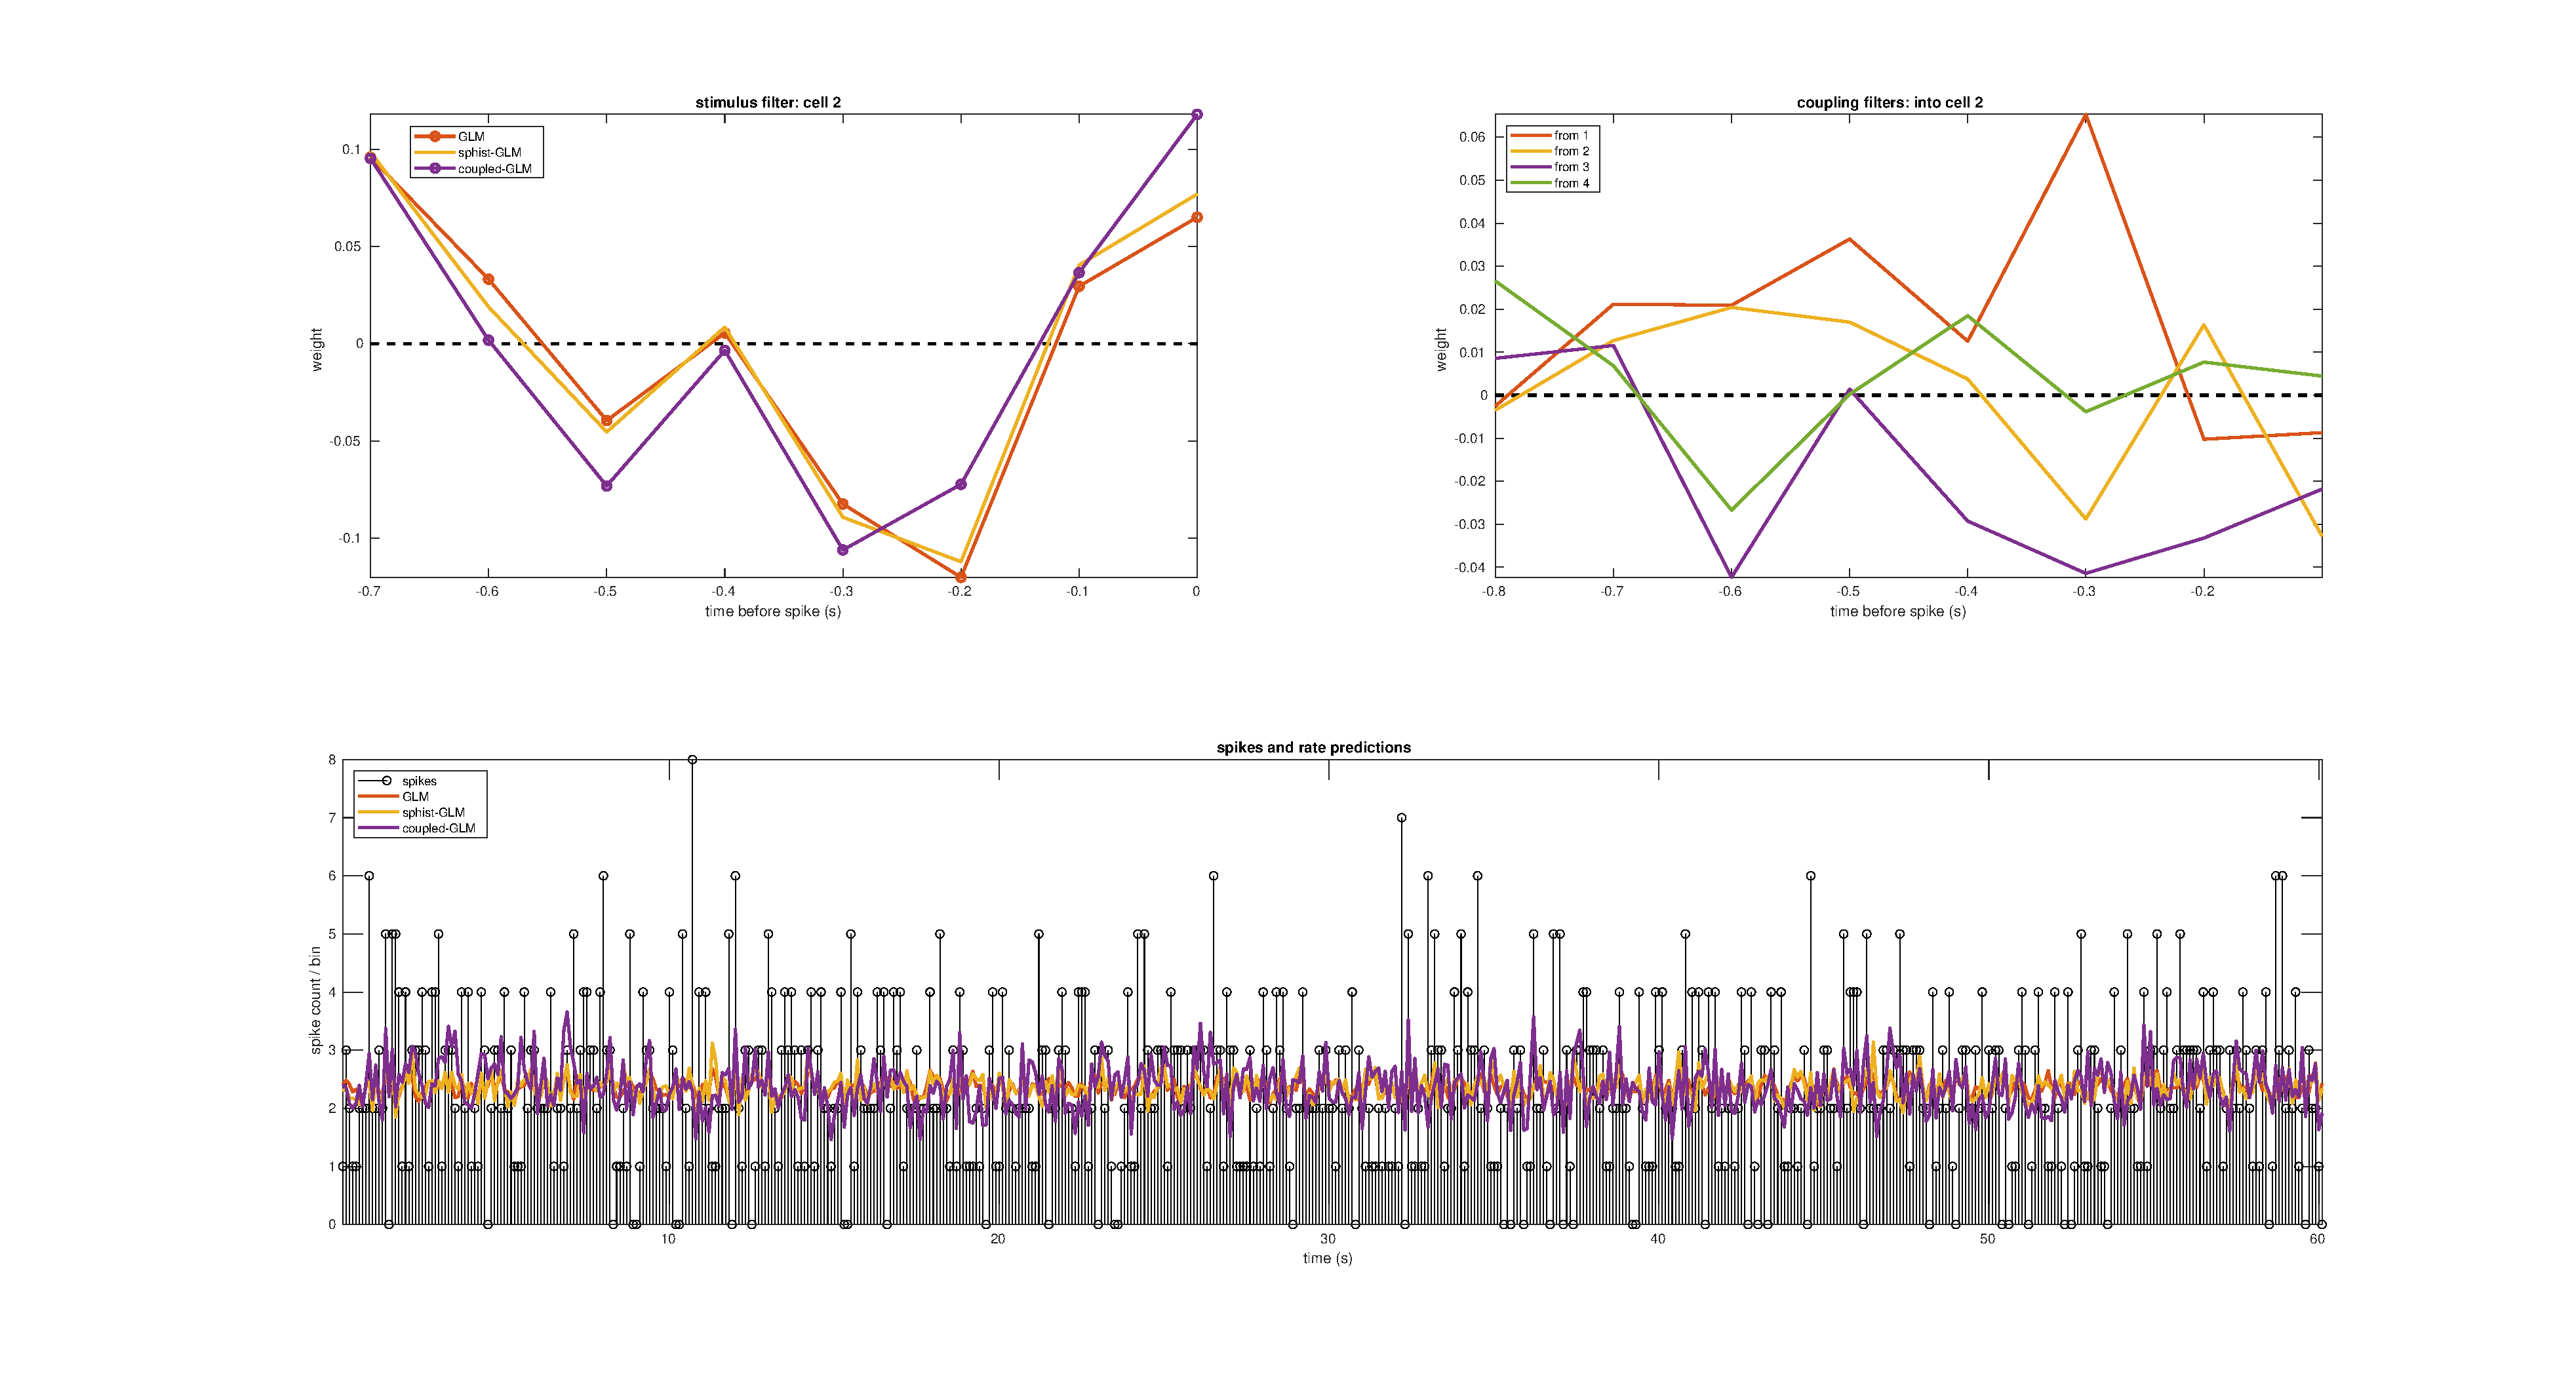
\includegraphics[width=1.2\columnwidth]{figures/matlab/export_GLM_filters_pred_bin_size_0_1_cell_2_target_GT_model_mesoGIF_N_4.eps}
%     \caption{A stimulus response filter, coupling filters, and spike train rate predictions for a GLM fitted to a population level (N=4) SGIF model.}
%     \label{fig:GLM_mesoGIF}
% \end{figure}
\begin{figure}
    \centering
    \vspace{-0.1in}
    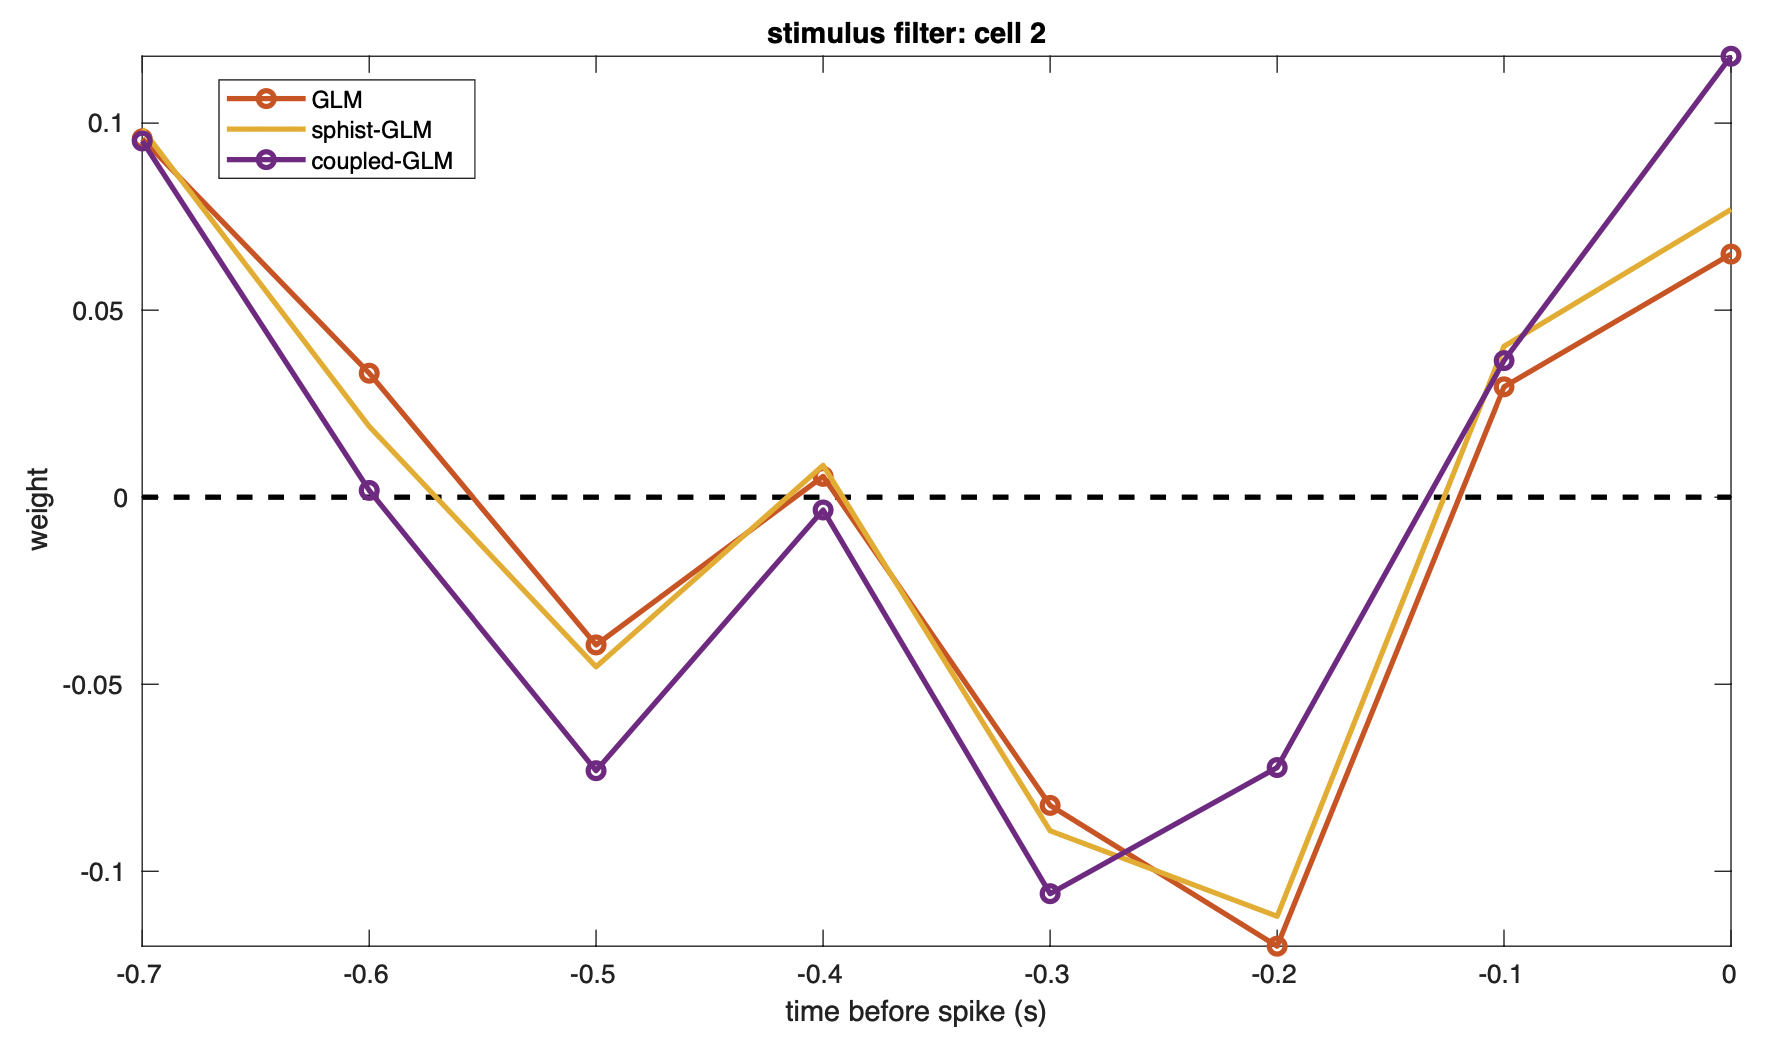
\includegraphics[width=0.8\columnwidth]{figures/matlab/font_fix/export_GLM_filters_pred_bin_size_0_1_cell_2_target_GT_model_mesoGIF_N_4_1.png}
    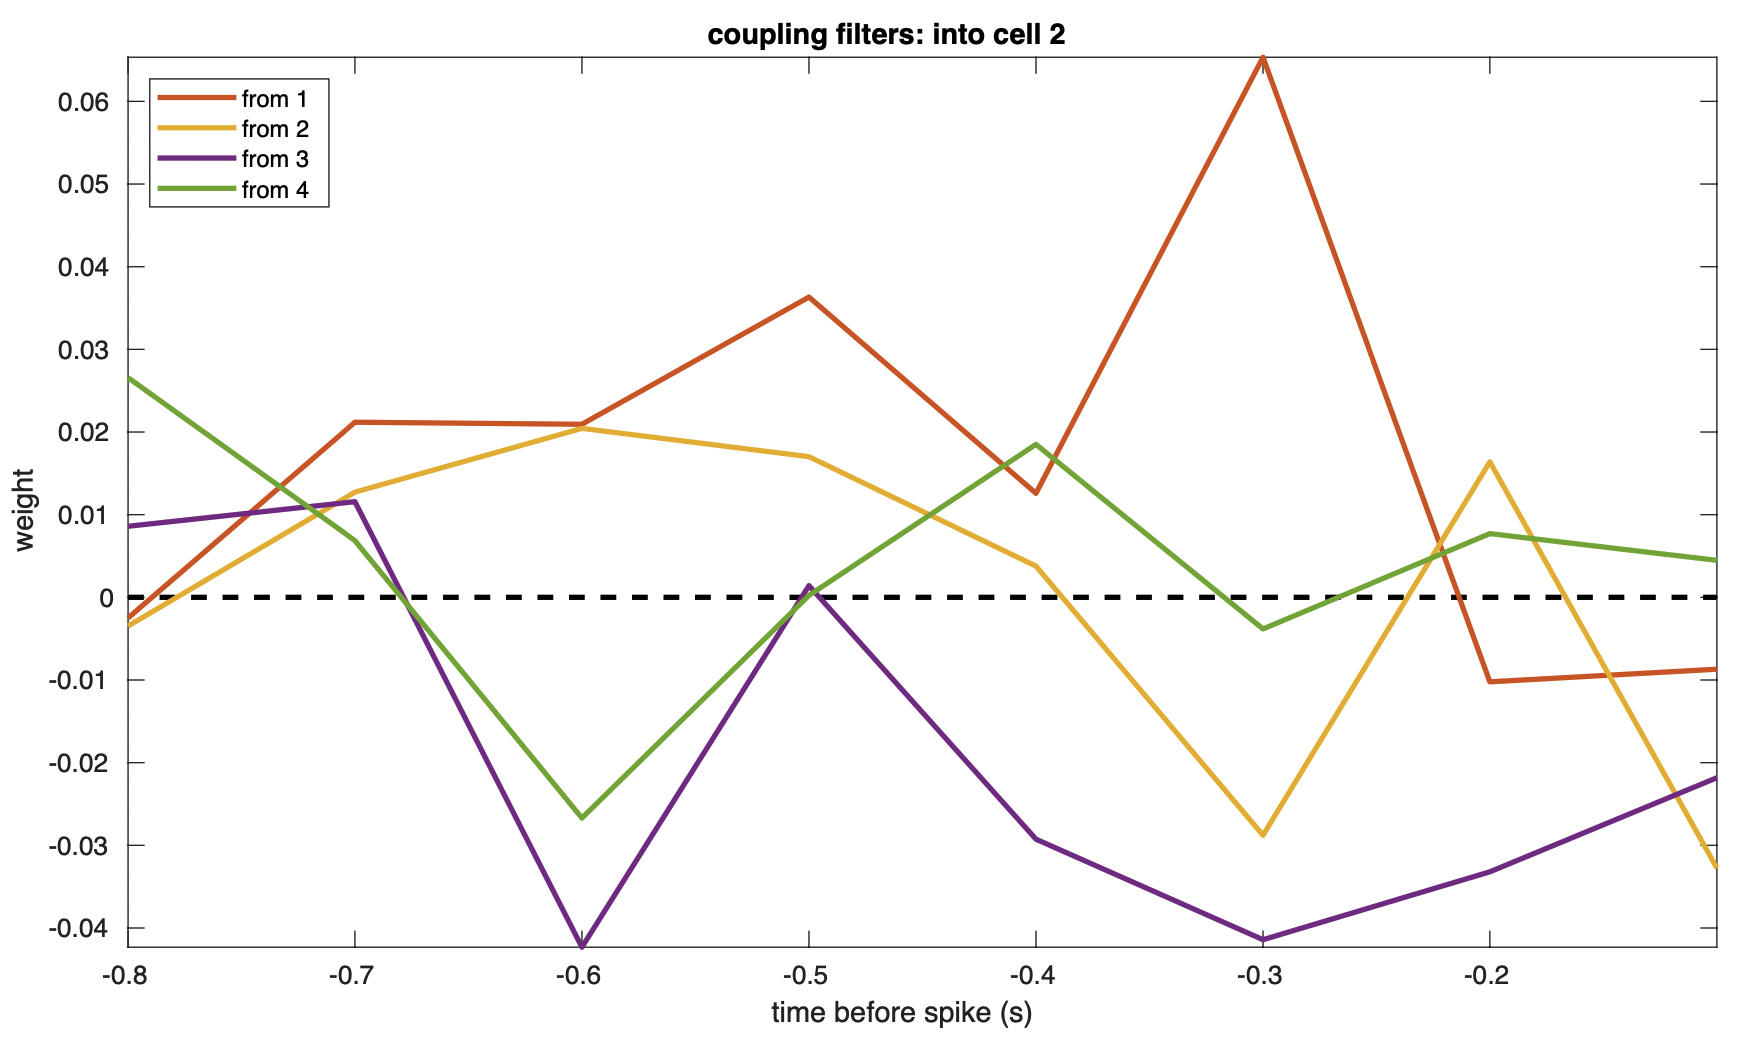
\includegraphics[width=0.8\columnwidth]{figures/matlab/font_fix/export_GLM_filters_pred_bin_size_0_1_cell_2_target_GT_model_mesoGIF_N_4_2.png}
    \vspace{-0.1in}
    \caption{A stimulus response filter and coupling filters for a GLM fitted to a population level (N=4) SGIF model.}
    \label{fig:GLM_mesoGIF_filters}
\end{figure}

\begin{figure}
    \centering
    \vspace{-0.1in}
    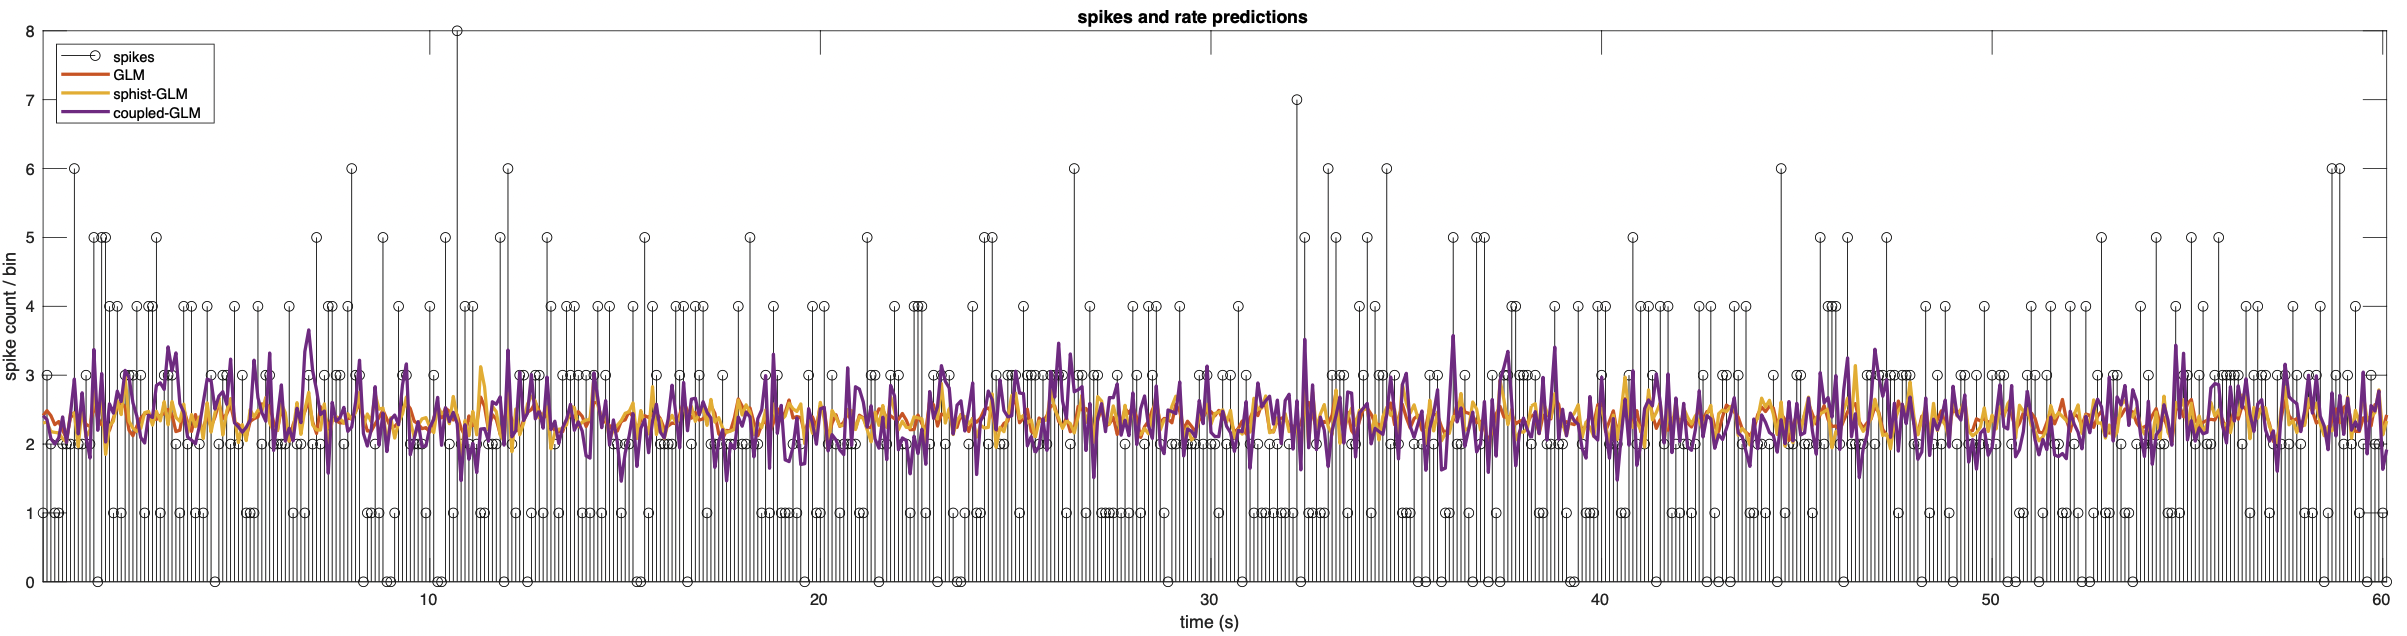
\includegraphics[width=1.7\columnwidth, angle=270]{figures/matlab/font_fix/export_GLM_filters_pred_bin_size_0_1_cell_2_target_GT_model_mesoGIF_N_4_3.png}
    \vspace{-0.1in}
    \caption{Spike train rate predictions for the fitted GLM where two of the response filters are illustrated in figure \ref{fig:GLM_mesoGIF_filters}.}
    \label{fig:GLM_mesoGIF_rate_preds}
\end{figure}

As a baseline model for assessing how well we capture higher-order spike statistics, we implement and fit GLMs as previously described (see section \ref{subsect:GLMs}), and also perform NMF (see figures \ref{fig:ACs_NMF_modules_mesoGIF_4}, \ref{fig:ACs_SGIF_N_21}, \ref{fig:modules_SGIF_N_21}) on the predicted spike trains of these models when perturbing them just as with the other models when generating their spike trains with white noise.
A sample figure of one of the neuron response filters of the GLM is shown in figure \ref{fig:GLM_mesoGIF_filters}, along with spike train rate predictions in figure \ref{fig:GLM_mesoGIF_rate_preds}.
Due to the fairly low-dimensional nature of the LIF model, MLE for a coupled Poisson GLM fits almost perfectly to the generative target LIF model.
Both SBI and GBO also perform fairly well for this model class in terms of the geodesic similarity (see figure \ref{fig:geodesic_all}).
However, when considering the more complex GLIF model class, which may exert a wider range of spike patterns and behaviours, the GLM performs slightly worse than GBO using a rate-based metric.
Interestingly, it performs just as well for both small and large SGIF networks, as the limit there seems to be the stochasticity introduced in this model class.
It is however outperformed for smaller SGIF networks by both GBO and SBI using NLL minimisation, but performs slightly better than GBO for larger networks.


\begin{figure}
    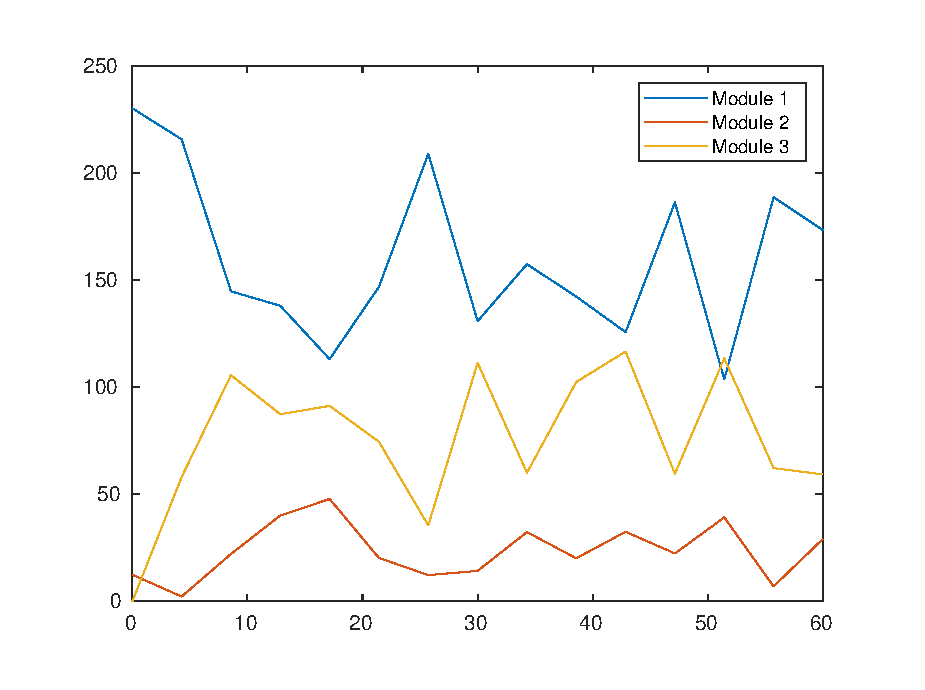
\includegraphics[width=0.65\columnwidth]{figures/matlab/NMF/ACs_target_GT_model_mesoGIF_N_4.eps}
    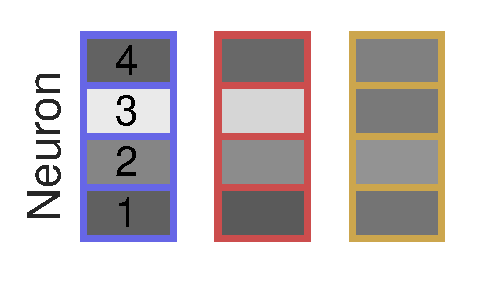
\includegraphics[width=0.3\columnwidth]{figures/matlab/NMF/target_GT_model_mesoGIF_N_4.eps}
    \centering
    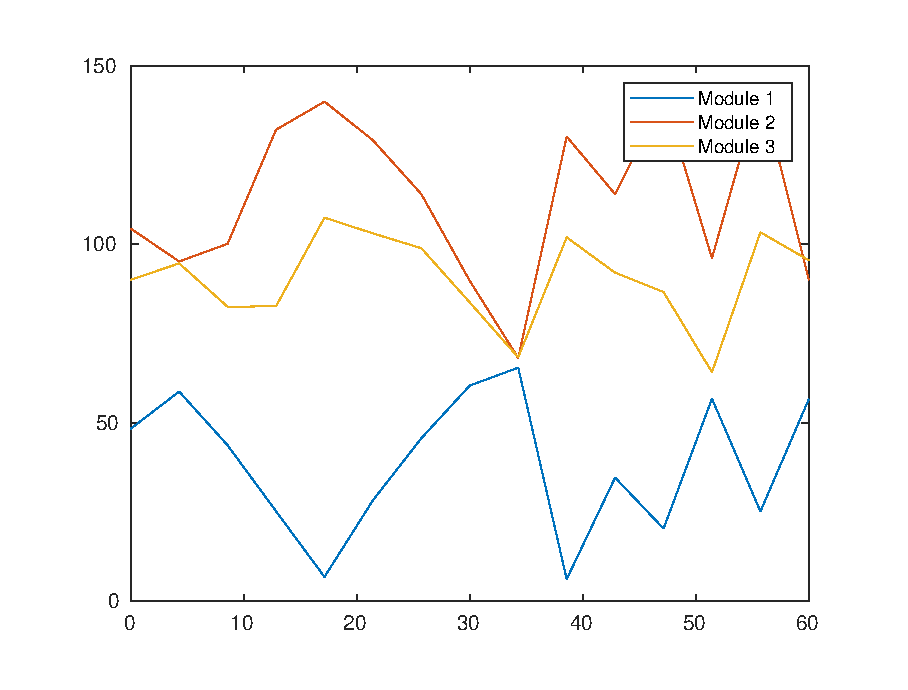
\includegraphics[width=0.65\columnwidth]{figures/matlab/NMF/ACs_nuovo_spikes_mt_microGIF_euid_12-09_16-02-03-400_lfn_bernoulli_nll.eps}
    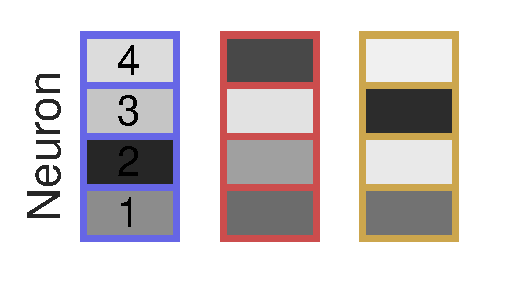
\includegraphics[width=0.3\columnwidth]{figures/matlab/NMF/modules_nuovo_spikes_mt_microGIF_euid_12-09_16-02-03-400_lfn_bernoulli_nll_4.eps}
    \caption{Activation coefficients (ACs) (top, seconds along the x-axis, and activation coefficient along the y-axis) for SGIF models, N=4, for target (top) and fitted models (bottom), using the Bernoulli negative log-likelihood (NLL) as the loss metric, along with the factorised NMF modules (right).}
    \label{fig:ACs_NMF_modules_mesoGIF_4}
\end{figure}

\begin{figure}
    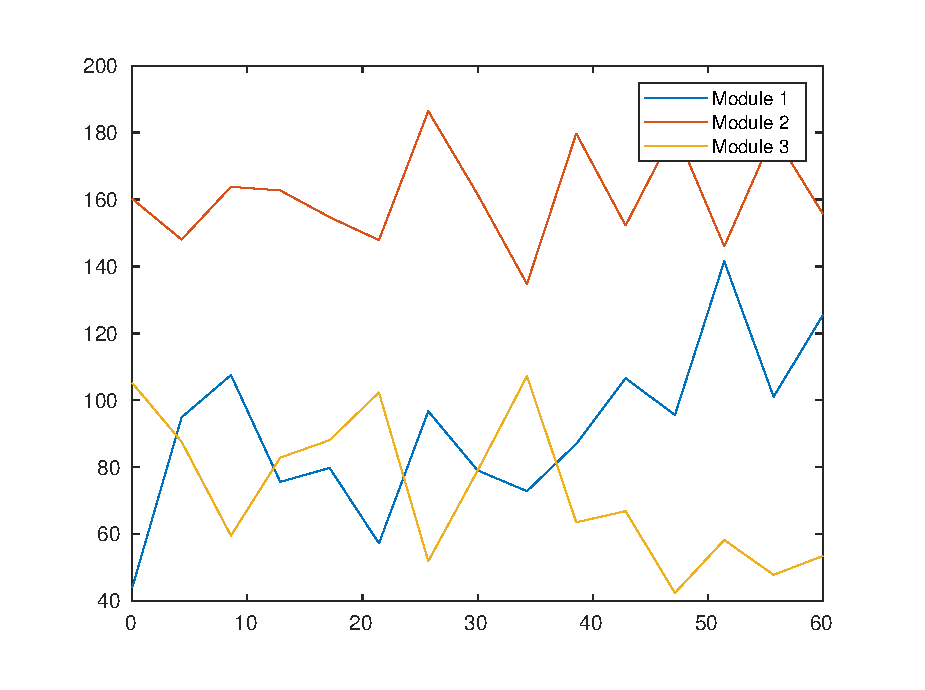
\includegraphics[width=0.65\columnwidth]{figures/matlab/NMF/ACs_target_GT_model_microGIF_N_21.eps}
    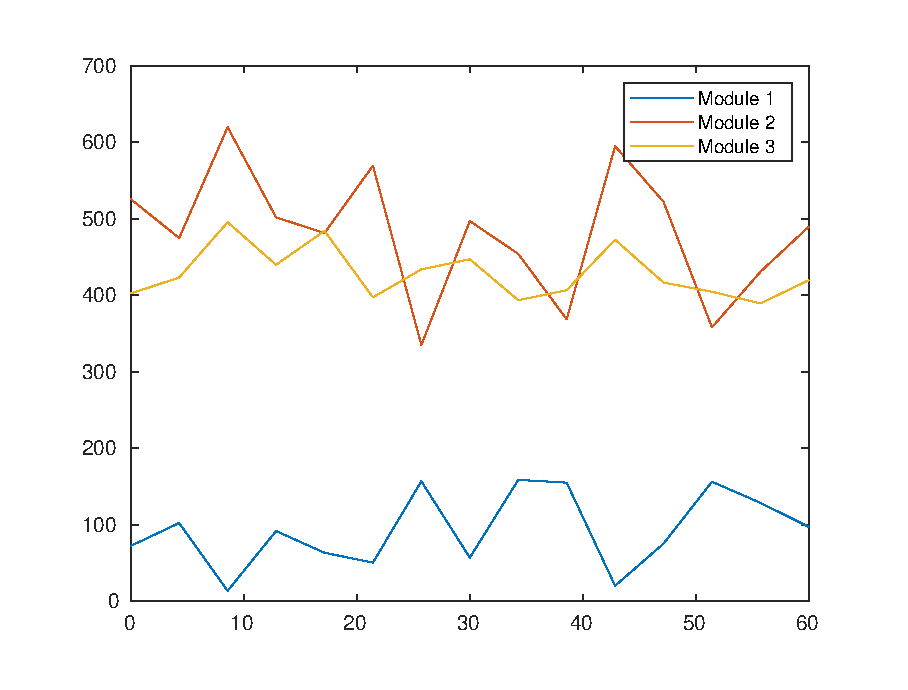
\includegraphics[width=0.65\columnwidth]{figures/matlab/NMF/ACs_nuovo_synthetic_v2_spikes_mt_microGIF_lfn_bernoulli_nll_euid_01-01_15-56-11-305.eps}
    \caption{Activation coefficients (ACs) (top, seconds along the x-axis, and activation coefficient along the y-axis) for SGIF models, N=21, for target (left) and fitted models (right), using the Bernoulli negative log-likelihood (NLL) as the loss metric, with the factorised NMF modules plotted in figure \ref{fig:modules_SGIF_N_21}.}
    \label{fig:ACs_SGIF_N_21}
\end{figure}

\begin{figure}
    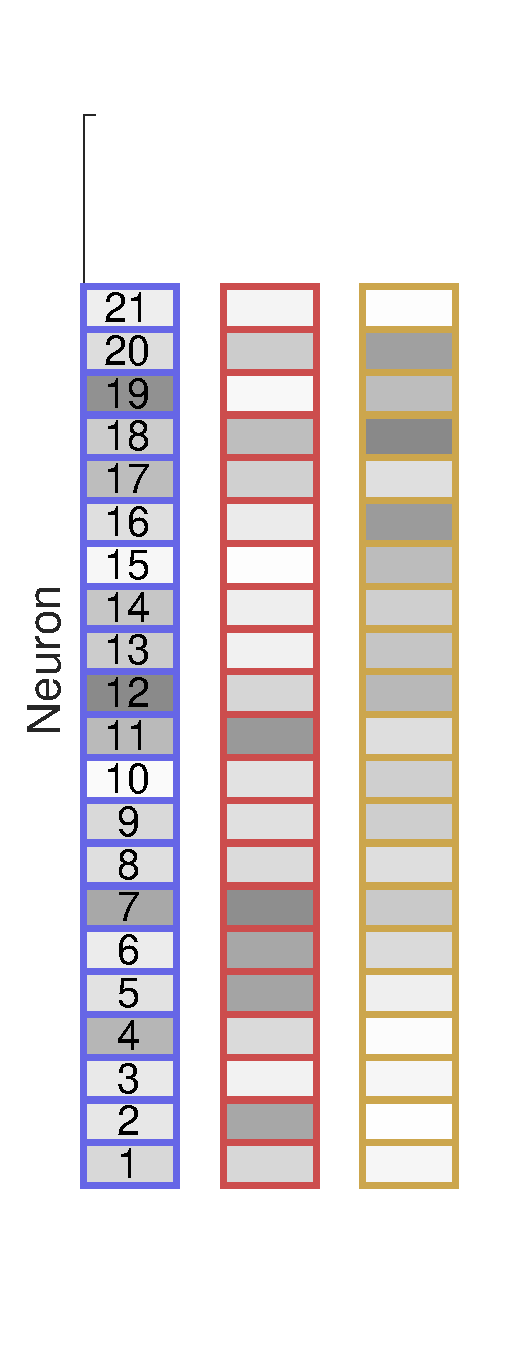
\includegraphics[width=0.3\columnwidth]{figures/matlab/NMF/modules_target_GT_model_microGIF_N_21_4.eps}
    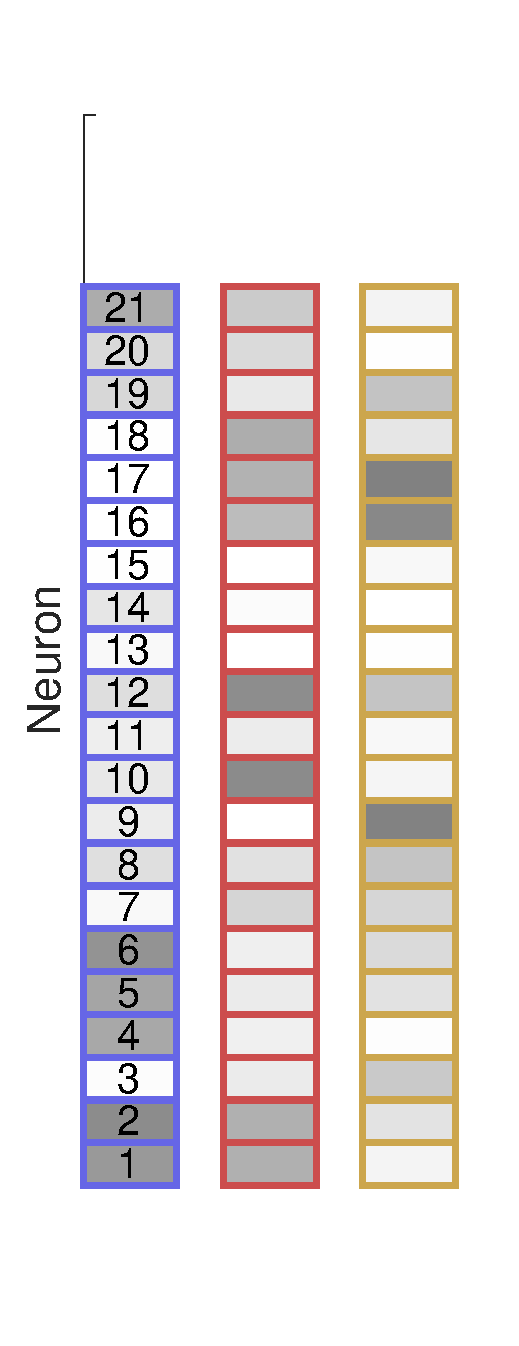
\includegraphics[width=0.3\columnwidth]{figures/matlab/NMF/modules_nuovo_synthetic_v2_spikes_mt_microGIF_lfn_bernoulli_nll_euid_01-01_15-40-04-701.eps}
    \caption{The NMF modules for the SGIF models, N=21, target (left) and fitted (right), using the Bernoulli NLL as the loss, as plotted (for the ACs) in figure \ref{fig:ACs_SGIF_N_21}.}
    \label{fig:modules_SGIF_N_21}
\end{figure}


\begin{figure}
    \hspace{-0.1\columnwidth}
    \vspace{-0.3in}
    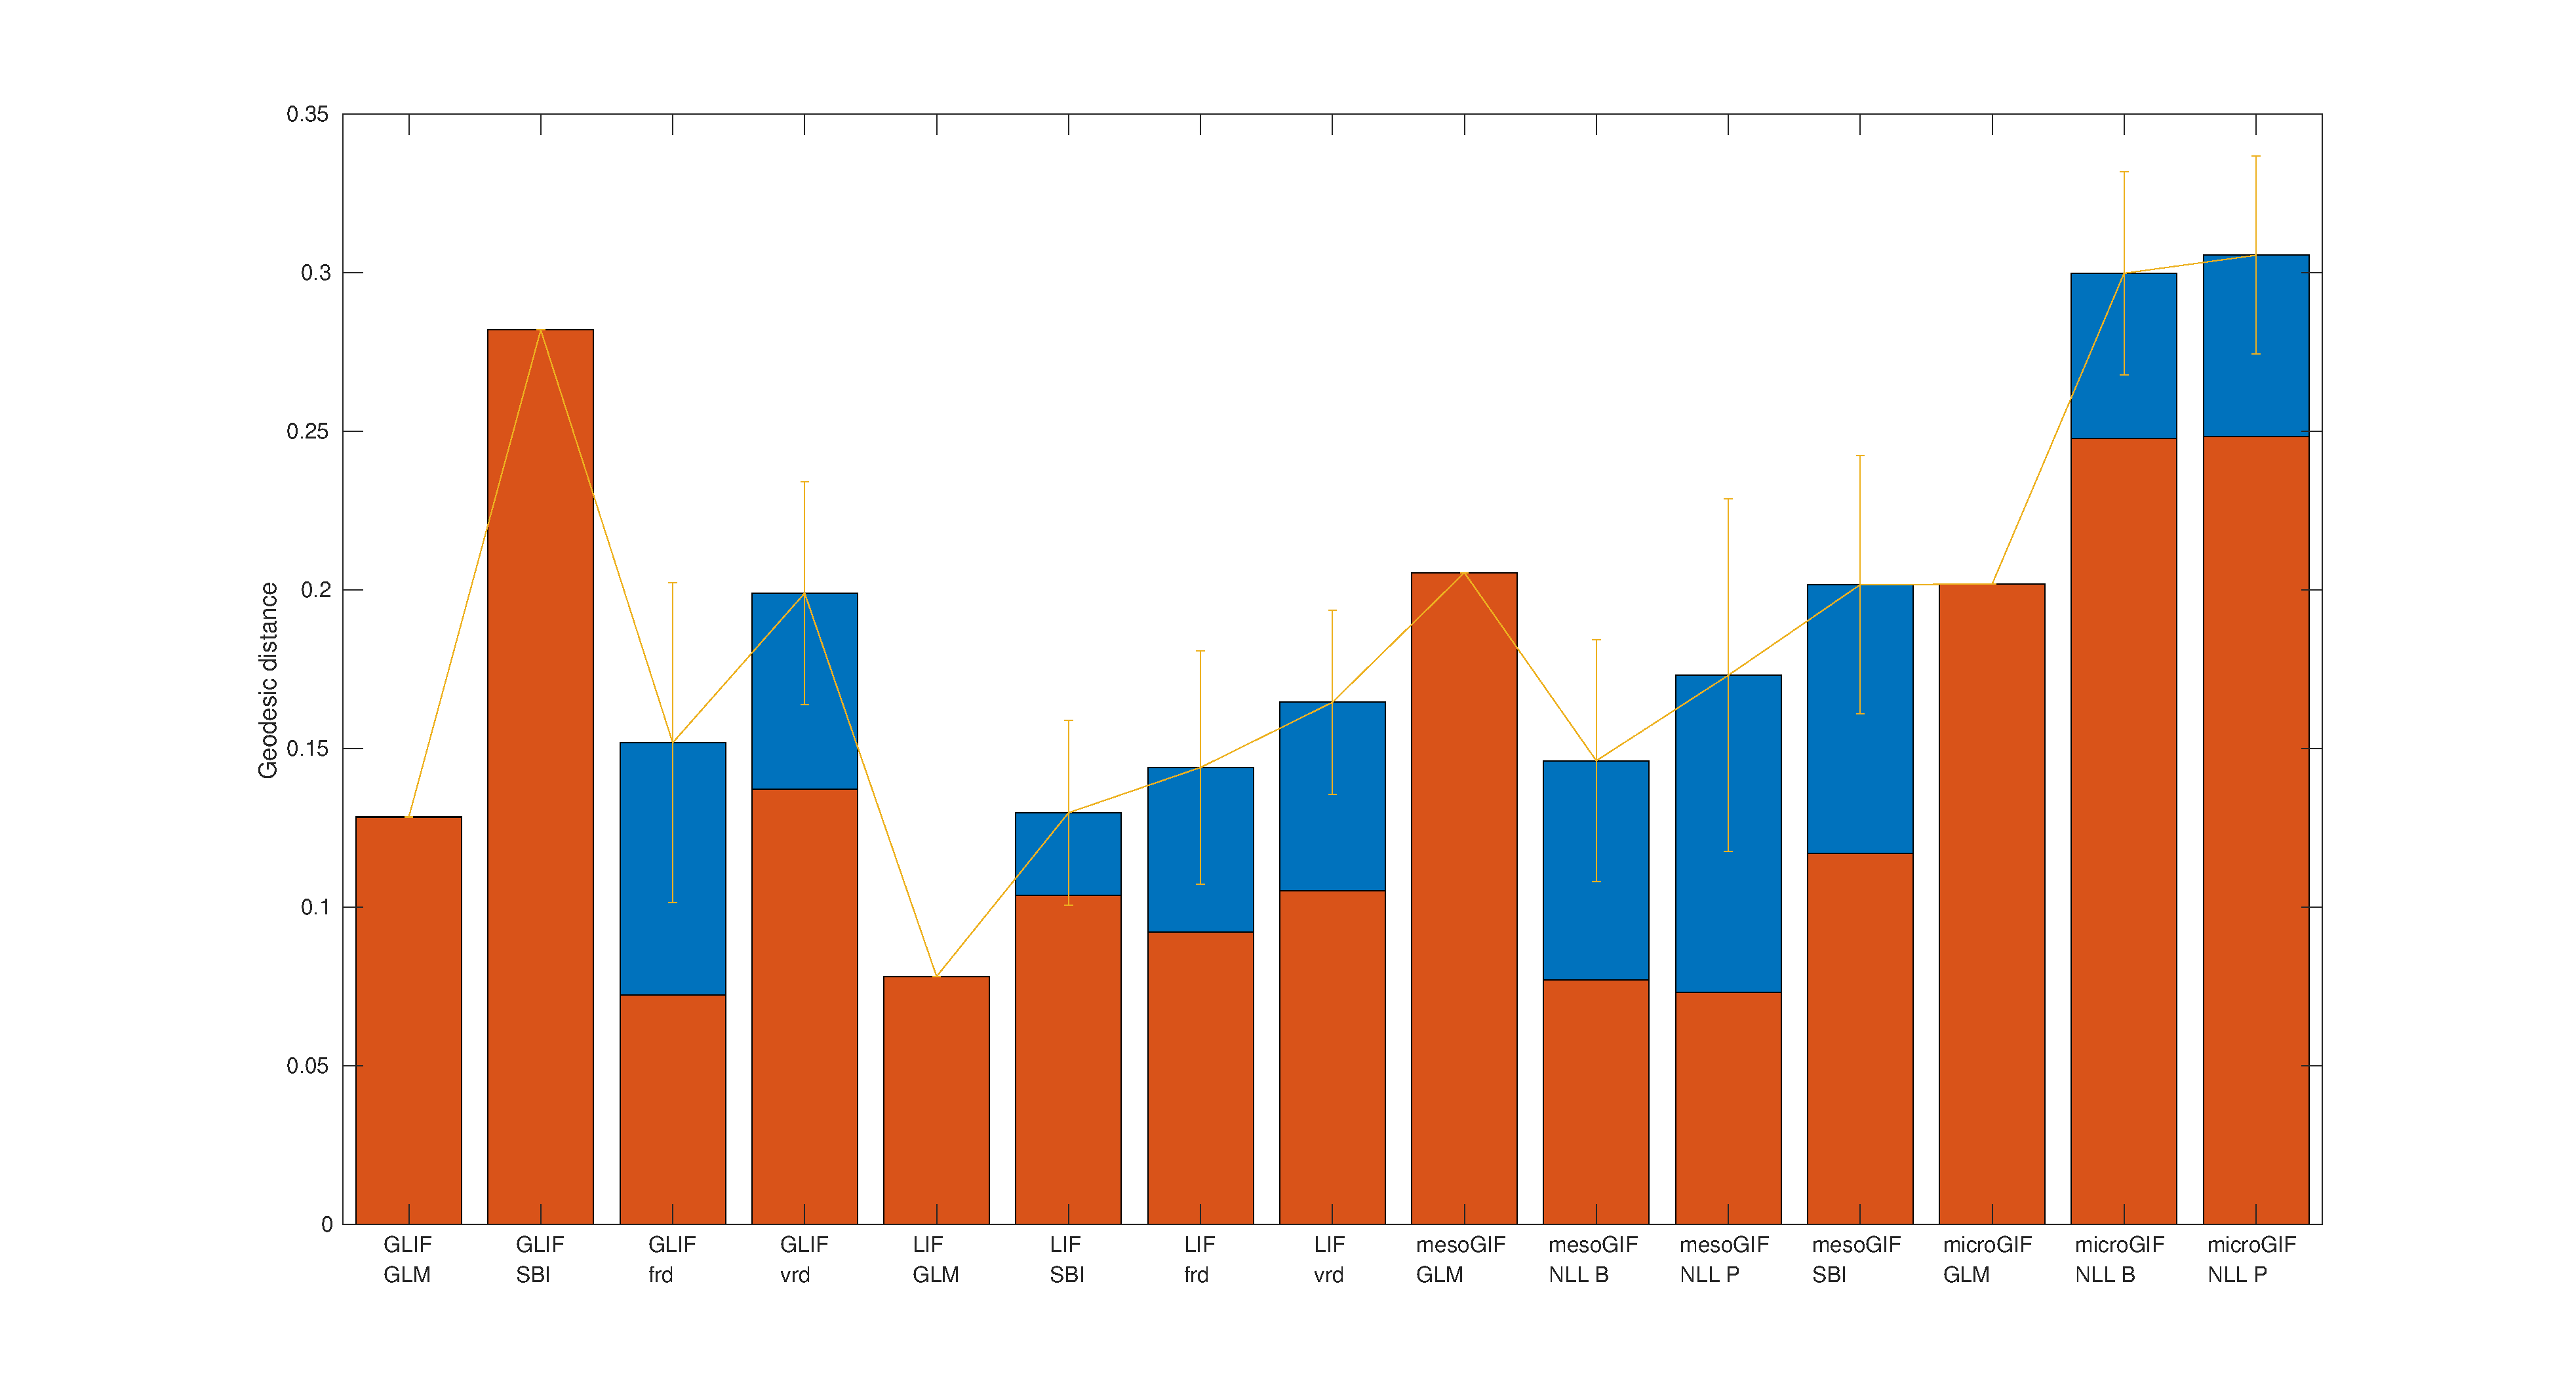
\includegraphics[width=1.75\columnwidth, angle=270]{figures/matlab/NMF_geodesic_all_Synthetic_v2.eps}
    \vspace{-0.3in}
    \caption{The geodesic distances between the NMF modules for all synthetic experiments.}
    \label{fig:geodesic_all}
\end{figure}


\section{Discussion}

The results showing that for GLIF and SGIF SNNs, the fits are better than for LIF SNNs may be somewhat counter-intuitive, but may be explained by considering that although we introduce greater complexity via the higher number of parameters for the GLIF and SGIF models, their formulations are also more robust in terms of the behaviours they may exhibit.
This may be further emphasised by considering our empirical data from trying to apply GBO to the Izhikevich model, discussed in section \ref{section:izhikevich}, in which we observed that fitting this model was highly challenging due to parameter regions for which model behaviour would be completely chaotic.
This is due to that the model is a lower-dimensional, collapsed projection of a system designed to be able to exhibit a myriad of behaviours (namely the Hodgkin-Huxley \cite{HH1952} model), but it comes at the cost of introducing regions in this projected system for which impossible and chaotic behaviours emerge.

The mean posterior marginals between the parameters in figures \ref{fig:mean_posterior_marginal_SNPE_LIF}, \ref{fig:mean_posterior_marginal_SNPE_GLIF}, \ref{fig:mean_posterior_marginal_SNPE_SGIF} show that similarly as for GBO, and as illuminated by the parameter error landscape plots, we fail to retrieve the ground-truth parameter means.
We are able to do so to some extent for the lower-dimensional (both in terms of parameters and number of neurons) LIF model, but cannot hope to meaningfully, i.e. with a strong link, interpret the values in a biological context for the inferred model.

The sample GLM plot shows illustrates that we may infer sensible stimulus filters and couplings using the MLE procedure (see section \ref{subsect:GLMs}), and illustrates a predicted spike train using a few different GLM variants.
This forms as previously discussed a baseline model that may be used when assessing whether our inferred SNN models may be more useful with regards to capturing higher-order statistics.

For evaluating whether we have the captured spatiotemporal structure of the spike train data, we perform NMF on the predicted as well as target spike trains for the different models.
As illustrated in figures \ref{fig:ACs_exp5}, \ref{fig:ACs_exp7}, we may factorise three ensembles of co-active neurons into modules of varying activity.
When evaluating their spatial similarity, we find a higher degree of similarity between the modules factorised from the spike trains predicted by the SNN models inferred using GBO.
Further, we also note that the activation coefficients of these modules bears similarity for the corresponding (most similar) module to some extent, which further suggests that we may have captured some of the functional organisation of the neurons in the original spike train data.
However, there is still a significant dissimilarity between the spatiotemporal factorised ensembles, and interpretations of the model such be constrained correspondingly.
Further, taking into account the aspects pertaining to the training signal, as well as the synapse model as discovered in the work extending \cite{Huh2018} as presented in chapter \ref{chpt:gated_synaptic} should be incorporated in order to try and better the similarity further.


\subsection*{Stochasticity and SNNs}

There usually is a larger space for which performance given by the loss metric is fairly equal (as depicted by the error landscape plots), just requiring a different combination of parameters - i.e. there is no single fixed point or trajectory leading to it in the parameter landscape leading to a global minimum.
One interpretation of this is that what we identify with learning algorithms for SNNs is not a specific configuration which captures the data set at hand, but a configuration which reaches a mode of behaviour that would allow it do produce the data.
% \subsection*{Implications for representational drift and sloppiness}
Interestingly, this is in line with the observed phenomena of representational drift whilst maintaining structural stability in the (functional) population patterns of activity \cite{Deitch2021RepresentationalCortex} in that in this work neurons aren't constrained to one configuration (or mode of behaviour) in order to participate in an ensemble, capturing patterns stably on a population-level.
If we want to take this one step further, it may even indicate that specific "fixed" neuronal representations when it comes to single-neuron activity (and synthetically its parametrisation) is not meaningful, or at least would not allow for the rich behaviour that we see in biology. One may imagine that if each neuron would only allow a fixed representation, this could quickly result in disastrous effects on the network-level, rendering the network incapable of capturing patterns of activity. For further reading on the robustness of networks of spiking neurons, the reader might be interested in the principle of tensegrity, which is eloquently described by \cite{Buzsaki2006}.

% Sloppiness
One of the motivations for investigating SNN model inference with GBO was the high performance in parameter inference noted by \cite{Teeter2018a}, allowing for classification of cell type based on the inferred parameters.
However, the aforementioned work pertains to a setting of single-neuron inference (and detailed neurophysiological data).
In the literature on sloppiness, single neuron properties and connectivity may change significantly whilst the population-level activity remains stable \cite{Panas2015SloppinessNetworks}.
Interestingly, in this view it might be expected to observe and attain sloppy regions in the error landscape on a network level - in contrast to on the single-neuron level.
% Not only are our observations in line with observations about representational drift, but also with sloppiness. 
% This may suggest that population-level configurations are a 
There are multiple ways one might interpret that networks are capable of learning tasks irrespective of single-neuron changes: 
In one view, the network-level signal is not sufficient for calibrating the single-neuron behaviour and parameters - for this, some more fine-grained signal is required. Note however that this view posits that the 'goal' of a neuron is to learn a specific representation, or similarly specific responses or behaviours, which is in contrast with the observation of representational drift.
Another way of viewing this that is more in line with the observation of representational drift is that neurons may change their responses, whilst yet successfully participating in e.g. performing a task on a higher (network and ensemble) level.
% \cite{Panas2015SloppinessNetworks} hypothesise and note that as long as some neurons remain 'central' and relatively active in an ensemble, they may drive synchrony and thus organisation in the network.
One hypothesis that comes to mind in this regard, is regarding the driving force behind learning representations and tasks.
Since neurons may change their responses naturally and more quickly than the network as a whole, which is naturally a lot stabler due to being the combination of all neuronal activities, resulting from all neurons' parametrisation and wiring, perhaps it is the representational drift in itself that allows for exploration, and the observed sloppiness in the error landscape on the network level that allows the relative functional stability (i.e. exploitation) throughout exploration and learning.


\subsection*{Multi-layer versus single-layer SNNs}

While multi-layer nets may be crucial for non-linear function approximation this work only considers fully connected "single-layer" SNNs.
Thus, testing the approach for multi-layer SNNs might give new interesting insights, and may also enable more easily capturing more complex data.
Perhaps this is one of the key missing pieces for taking the step from the succesful optimisation of the models when fitting to a lower-dimensional signal, as studied in chapter \ref{chpt:gated_synaptic}, to fitting directly to target spike trains?


% Preliminary conclusion: 
The spatiotemporal nature of SNNs, with the main measured effect being a function over a highly composite variable that has a high temporal dependency and variability, may complicate optimisation.
In addition to being highly sensitive to initial conditions and other factors potentially both skewing the times of spiking, as well as the very mode of behaviour and spiking, input-output transformations, and the spatiotemporal signature of spike trains need to be handled in a way that is robust to these perturbations. 
% Currently, there seems to be no defined loss metric that may capture the distance and resulting parameter landscape when going from one mode of behaviour to another in network nodes in a way that is exploitable by means of gradient based optimisation.
A large number of our experiments revolved around trying to facilitate for ground-truth paramater retrieval.
However, the results show that ground-truth retrieval is highly unlikely with the specified model definitions and loss metrics.
By constructing error landscape plots in \ref{sect:e_landscapes}, we illuminate why this is.
Interestingly, although local minima are inferred with regards to the parameter values, these configurations may yet capture the spike train statistics of the target data, as demonstrated by applying the dimensionality reduction technique of NMF to compare the ensembles of coactive neurons in the spike trains predicted by the inferred models.
Thus, the scalable approach of GBO may be leveraged in this regard, and bears potential for future work for automating and accelerating SNN inference work.
The results highlight that the procedure is feasible by demonstration a working implementation and integration of various model classes, for both stochastic and leaky integrate-and-fire, and highlight that a stricter definition of the model perturbation scheme, as well as a more informative loss metric design, may be key to improving inference performance.


% =======================================================
% =======================================================
% =======================================================
\chapter{Sleep regulation in the rodent brainstem}\label{chpt:sleep}

My initial research proposal outlines a research project where the goal is to meet research needs within the field of sleep regulation through computational modelling.
In this chapter, we apply the inference methodology of this thesis pertaining to spike based SNN inference using GBO to biological spike train data, recorded from the brainstem of mice during different vigilance and sleep states, and assess to what extent the higher-order NMF modules, which correlate with the brain state, are captured in the inferred models.

More specifically, the aspiration was to model neurons of the pedunculopontine and laterodorsal tegmental areas within the brainstem during different brain states, based on their neuroanatomy as described, even though scarcely, within the literature, and based on in vivo data from these brain areas \cite{Herice2019c, Tsunematsu2019, Pal2007, Martinez-Gonzalez2011, Fraigne2015}.
Further, an overarching research goal was to be able to capture the emergence of neural ensembles as identified in vivo in the model by using non-negative matrix factorisation (NMF) \cite{Seung1999, Seung2001, Onken2016a}.
To this end, we have implemented various types of SNN models, a framework for gradient based optimisation using Adam in a modular way, compatible with any differentiable model as well as loss metric, all in PyTorch. This work is presented previously in this dissertation.
Further, the hand-engineered target models that were used to test the methodology whilst also maintaining the ground truth generative model parameters in chapter \ref{chpt:frontier} were designed to have neuronal rates and parameter values resembling a mixture of excitatory and inhibitory neurons, keeping both biological data and the particular sleep data in mind.
More generally, computational modelling and spiking neural network (SNN) inference covers several research needs within the field of sleep research and the synthesis of neuroscience and its computational counterpart in that it addresses model scarcity, as well as a methodology for accelerating modelling by inference through gradient-based optimisation \cite{Herice2019c, Huh2017, Taherkhani2020}.
This was the foundation for sparking my interest in a methodological project in the first place, with the goal of automating biologically relevant neural network model inference, and more specifically to research both (1) the current state-of-the-art on SNN inference, and (2) leveraging ML based methods of gradient descent and optimisation for SNN inference \cite{Huh2017, Mostafa2020, Tavanaei2019b, Lee2016}.

While it is evident that the extent to which GBO may be used to infer an exact SNN model based on spike data from the findings in the previous chapter, the results nevertheless show that the approach may infer models that capture the higher-order statistics and functional organisation fairly well, and even better than a solid baseline model, namely the GLM.
As the ABC approach of SNPE quickly becomes intractable, and is in fact intractable for the network size of the biological data studied in this chapter (at least for a reasonable execution time, with limited computational resourced), we have employed our GBO procedure to biological spike train data for LIF, GLIF, and SGIF models, and similarly to in the previous chapter, we assess the goodness of fit via the attained model rates, loss, and geodesic NMF module similarities.

\section{Background}

Sleep is widespread across different animal species, crucial to mental functioning \cite{Brown2012, Walker2018}. 
However, why and how we sleep, remains to be understood, with a rich literature pertaining to different aspects of sleep, its regulation, potential functioning, and different pathways \cite{Borbely1992, Fraigne2015, Brown2012, Herice2019a, Watson2011a, VanDort2015, Hobson2002, Narwade2017, Klinzing2019, Dunmyre2014, Costa2016, Halgren2019, Eban-Rothschild2018, DeVivo2017, Weber2018, Herice2019c, Keene2018, Scammell2017, Cox2016, Grace2014, DinizBehn2010, Anafi2019, Callaway1987, Lim2007, Mallick2001, Ni2016, Pal2007, VanDort2015, Gonzalez2019, Weber2016, Herice2018, Song2019, Pal2005, Tsunematsu2019, Fleshner2011, Datta1997, Buzsaki2015, Theodoni2018, Hoel2021, Hopfield1983, Kinouchi2002, Martinez-Gonzalez2011}. 
Some models exist that seek to capture the phasic nature of sleep, but mostly at an abstract level. 
There is as such a need for detailed models in the field, with no current models encompassing direct biological parallels. Addressing the need for modelling in the field, and seeking to illuminate how we sleep, we propose to use a set of recently combined methodologies that allow us to infer neuron-level spiking models based on recorded spike trains. 
The methodology allows for incorporating both existing knowledge from the ML domain, and lays the groundwork for using GBO for SNN inference, illuminating the extent to which this may be done with the proposed methodology, as well as highlighting key issues that should be adressed in future modeling work along this strand.
The outlined algorithmic approach applied to spike train data has, to the best of our knowledge, not been previously explored. 
This may be due to the high dimensional parameter search space, which also complicates making inference tractable and sufficient.
% The approach requires only partial data - as is always a constraint within neuroscientific recordings. 

\subsection{Sleep stages}

When it comes to the phasic nature of sleep, one seminal yet simple model for describing this is a three-process switch or flip-flop model, as described by \cite{Borbely1992}.
This describes how a combination of a homeostatic drive, the circadian (24-hour) rhythm, and an ultradian rhythm may facilitate and regulate sleep, wakefulness, and the different types of sleep (namely NREM- and REM-sleep), without detailing the pathways involved.
% Different timescales may be at play, and constitute the switching-mechanism.
This begs the question of whether an inferred SNN be used as a starting point to create such a model, or whether it can be determined to be involved in one or more of the three hypothesised regulatory mechanisms.

\subsection{PPT/LDT}

Many areas have been thoroughly researched with regards to their role in sleep regulation, such as the locus coeruleus (LC) \cite{Mallick2001, DinizBehn2010, Brown2012, Khanday2016a}, which is fairly well understood.
However, other areas which have been shown to be involved in sleep regulation are less or poorly understood.
One such area is the pedunculopontine and laterodorsal tegmental areas (PPT/LDT) of the brainstem, with its circuitry containing a myriad of inputs and outputs \cite{Pal2005, Brown2012, VanDort2015, Herice2019a}.
Could these be modeled by inferring models that reproduce similar spiking activity by using GBO with data recorded by silicon probe insertion into the area?
If so, to what extent can we reverse-engineer the neural activity, classify the neurons into types, and illuminate the pathways involved, such as whether the neurons facilitate REM-sleep or not - i.e. are REM "ON" or "OFF"?
While it is limited what we can capture in the current model, one thing that is out of scope for this thesis, but would be straightforward to implement, is designing input that more closely resembles that of during REM- and NREM-sleep.
This could then be presented to inferred models, and if captured by the inferred model, the ensembles could tell us something about state-regulation.
% If so, the can be identified, parameters compared and fixed, and then we could try to reconstruct the projections.

% PPT/LDT LFP data; most spiking during NREMS
% (to consider: Little time spent in NREMS)
% Want to primarily look at REMS: disinhibition of monoaminergic LC projections (prerequisite; Timofeev et al. (2017)) (shut off / inhibited in LC by GABA), 

% PPT/LDT:
% Cholinergic are REMS and wake
% GABAergic; REMS, wake, or both
% NREM?


\section{Biological target data}
\label{subsect:bio_data}

The biological data that we were granted access to is from a silicon probe recording (8x4 Buszaki probes) from the PPT/LDT area of the brainstem. 
It is analysed in published research, in which evaluation and assessment through rigorous analysis and classification and prediction of the future brain state given the neuronal signals, as well as NMF modules, was performed \cite{Tsunematsu2019}. 

We here replicate much of the results of \cite{Tsunematsu2019}, confirming that NMF ACs were more indicative of future brain state than HPC signals, which was a novel finding and insight when presented in the original paper.
This also means that the data should contain information that if captured in a model may illuminate the functional dynamics associated with sleep regulation in the area (PPT/LDT).
% In order to test whether ...
% See first year(?) review
Further, we also tested and confirmed that single-neuron signals were slightly better predictors. 
However, as the gain is only marginal or small it also suggests that the ensembles are indeed good representations of the spike activity, and thereby functional ensembles, as argued in the original paper.
Therefore, we perform NMF on the predicted spike trains of our inferred models, and compare the factorised modules attained with those of the biological target data.
Note that the quality of the spike data in terms of neuronal activity and non-silent neurons varied across the different experiments.
So did classification performance with the aforementioned variability.
Therefore, we have focussed on the two experiments in which most neurons displayed activity, and the state classification performance was consistently high (see figures \ref{fig:lda_classification} and \ref{fig:lda_rf_classification}).
These were also the two only data sets for which three NMF modules were needed in order to account for at least $75$ \% of the variance in the original spike data with the factorised matrices.

\begin{figure}
    \centering
    \vspace{-0.1in}
    \includegraphics[width=0.7\columnwidth]{figures/LDA/lda_temporal_shifting_and_prediction_bins_4_lda_acs_temporal_windows_4_exp_6.eps}
    \vspace{-0.1in}
    \includegraphics[width=0.7\columnwidth]{figures/LDA/lda_temporal_shifting_and_prediction_bins_4_lda_acs_temporal_windows_4_exp_4.eps}
    \vspace{-0.1in}
    \caption{Prediction accuracy (second axis) by the time preceding the predicted state in seconds (first axis). The biological data often contained silent neurons, with the most consistently active signals and thus 'well-defined' data being particularly the data sets for experiments 4 and 6.}
    \label{fig:lda_classification}
\end{figure}

\begin{figure}
    \centering
    \includegraphics[width=0.7\columnwidth]{figures/LDA/bars_LDA_per_signal_t_3.eps}
    \includegraphics[width=0.7\columnwidth]{figures/LDA/bars_RF_per_signal_t_3.eps}
    \caption{LDA and random-forest classification over the different experiments.}
    \label{fig:lda_rf_classification}
\end{figure}

% Suggests spike statistics well captured in factorised modules, as ACs sufficient to predict brain state.
% Thus, functional ensembles should be well represented by modules, and be a correspondingly suitable methodology to assess capturing these by calculating the similarity of the factorised modules for fitted SNN models.
% As the similarity metric, we simply calculate the geodesic similarity between modules, as previously in the synthetic SNN inference work.

\clearpage
\section{Inference}

As mentioned above, we have focussed on the two experiments with consistently high 'quality' in terms of neuronal activity and vigilance state prediction performance.
Further, we adopt the differentiable SGIF-model as described in previous chapters \cite{Rene2020}, using GBO for direct neuron-level SNN inference by negative log-likelihood minimisation, assuming either a Bernoulli or Poisson distribution of the spike train.
For NMF performance evaluation between NMF modules (such as illustrated in \ref{fig:modules_exp5}, \ref{fig:modules_exp7}), we also fit GLMs (section \ref{subsect:GLMs}) as a baseline comparison model in NMF module similarity assessment (with the similarity distance plotted in \ref{fig:geodesic_distances_exp5}, \ref{fig:geodesic_distances_exp7}).

For each experiment, we fit $N=20$ models as in the other setups to each experiment, for each model type and loss function, pseudorandomly and uniformly initialising the model parameters before inference, with a different random seed for each experiment.
We here report the results for each configuration for the two data sets, in addition to illustrations of the fitted GLMs (figures \ref{fig:stimulus_response_filters}, \ref{fig:glm_sample_cell_5_exp_5}).

\begin{figure}
    \centering
    \vspace{-0.1in}
    \includegraphics[width=0.9\linewidth]{figures/sleep/plot_1_cell_5_subplot.png}
    \vspace{-0.1in}
    \caption{Response filters for the GLM, here fitted to experiment 5 data, with corresponding sample node filters shown in figure \ref{fig:glm_sample_cell_5_exp_5}.}
    \label{fig:stimulus_response_filters}
\end{figure}

\begin{figure}
    \centering
    \includegraphics[width=0.9\columnwidth]{figures/sleep/GLM_multi_cell5_5sec_bin_white_noise.eps}
    \caption{Filters for an arbitrary sample GLM cell and predicted spikes and rates for the GLM with different couplings for experiment 5 (the blue - "GLM" is the full GLM as used for the baseline in the NMF analysis comparison).}
    \label{fig:glm_sample_cell_5_exp_5}
\end{figure}


\begin{figure}
    \centering
    \vspace{-0.1in}
    \includegraphics[width=0.65\columnwidth]{figures/sleep/approx_rate_across_exp_microGIF_bernoulli_nll_vs_fitted.eps}
    \vspace{-0.1in}
    \includegraphics[width=0.65\columnwidth]{figures/sleep/approx_rate_across_exp_microGIF_poisson_nll_vs_fitted.eps}
    \vspace{-0.1in}
    \caption{Inferred model firing rates per data set for the SGIF model, using white noise with a fixed rate as input perturbation, Bernoulli NLL (top), and Poisson NLL (bottom).}
    \label{fig:approx_rates_sleep_exps_SGIF}
\end{figure}


\begin{figure}
    \centering
    \vspace{-0.1in}
    \includegraphics[width=0.8\columnwidth]{figures/sleep/ACs138.eps}
    \vspace{-0.1in}
    \includegraphics[width=0.65\columnwidth]{figures/sleep/ACs_SGIF_exp5_fit_bernoulli_nll_2.eps}
    \vspace{-0.1in}
    \caption{Activation coefficients (ACs) (second axis) by time in seconds (first axis) for experiment 5 for the target (left), and SGIF fitted model (right), using the Bernoulli NLL as the loss metric.}
    \label{fig:ACs_exp5}
\end{figure}

\begin{figure}
    \centering
    \includegraphics[width=0.3\columnwidth]{figures/sleep/modules138.eps}
    \includegraphics[width=0.3\columnwidth]{figures/sleep/modules_SGIF_exp5_fit_bernoulli_nll.eps}
    \caption{ACs for experiment 5 for the target (left), and SGIF model fit (right). These particular modules have a geodesic similarity of approximately $73 \%$.}
    \label{fig:modules_exp5}
\end{figure}

\begin{figure}
    \centering
    \includegraphics[width=0.65\columnwidth]{figures/sleep/geodesic_exp138.eps}
    \caption{Geodesic distances across model types and loss functions for experiment 5.}
    \label{fig:geodesic_distances_exp5}
\end{figure}

\begin{figure}
    \centering
    \includegraphics[width=0.8\columnwidth]{figures/sleep/ACs147.eps}
    \includegraphics[width=0.65\columnwidth]{figures/sleep/ACs_nuovo_sleep_v2_spikes_mt_microGIF_euid_12-29_02-12-29-631_exp_6_lfn_poisson_nll.eps}
    \caption{ACs (second axis) by time in seconds (first axis) for experiment 7 for the target (left), and SGIF model fit (right), using Poisson NLL minimisation.}
    \label{fig:ACs_exp7}
\end{figure}

\begin{figure}
    \centering
    \includegraphics[width=0.3\columnwidth]{figures/sleep/modules_exp147.eps}
    \includegraphics[width=0.31\columnwidth]{figures/sleep/modules_nuovo_sleep_v2_spikes_mt_microGIF_euid_12-29_02-12-29-631_exp_6_lfn_poisson_nll.eps}
    \caption{NMF modules for experiment 7 the target (left), and SGIF model fit (right). These particular modules have a geodesic similarity of approximately $69 \%$.}
    \label{fig:modules_exp7}
\end{figure}

\begin{figure}
    \centering
    \includegraphics[width=0.65\columnwidth]{figures/sleep/geodesic_exp147.eps}
    \caption{Geodesic distances across model types and loss functions for experiment 7.}
    \label{fig:geodesic_distances_exp7}
\end{figure}

The results show that we may infer a model where the rates match fairly well for each neuron, \ref{fig:approx_rates_sleep_exps_SGIF}.
Interestingly, the results also show that assuming a Poisson distribution and using this to optimise over the negative log-likelihood results in a significantly lower loss than when assuming a Bernoulli distribution: Student-T test (statistic=$9.87$, $p_{value}=6.23e^{-05}$).
This is in contrast to the work on synthetic target data, in which the best performance was attained by assuming a Bernoulli distribution when optimising over the NLL.
One possible explanation for this is that true biological data may be of a more complex nature, which is better described by a Poisson- rather than a Bernoulli-assumption.
% Elaborate more?

% \section{Neuroscience parallels for sleep regulation}
% Grace (14)
% Temporal structure ow cholin. Neur.s. can affect downstream
% Chemogenetic could not induce REMS
 
% Initiated in ACh PPT/LDT
 
% Denise originally architect. Costa et al. (16)
% - Main difference is time const. of synn. Response; shorter in orig. paper. Can mimic more rhodent-like state shift
% Funding bbsc
 
% Might apply for only neuro.
% Where is probe inserted – dyeing
 
% Phase-locked activities for delta-waves, too
% P-waves might occur during UP-state
% Phase-locked
% Principle of “computation”?
 
% (Principle derivation?)
% Cell paper information contents between cortex and amygdala in humans and monkey
% “A Tradeoff in the neural code across regions and species” January 2004
% Pryluk et al.
 
% Specific q could be: Role of cholin. Neurons. Temporal structure may be important for REMS
 
% Izhikevich instead of LIF for Grace
% Once they get REMS – state dependence from cholin. Circuitry too
% Temporal structure might be important

As the number of nodes is slightly higher for these data sets, the SBI ABC approach outlined in chapter \ref{chpt:frontier} is intractable for the data at hand, and is thus out of scope for the biological data. 


\section{Discussion}

% Direct microscopic model inference tractable for non-dales law compliant models by using GD and Adam over a rate-based metric for (G)LIF models, and over the negative log-likelihood for stochastic models.
% Local minima wrt parameters as shown previously with known GT, however, when considering the NMF ensembles captured through the two approaches,

This chapter demonstrates the scalable and modular GBO approach applied to biological spike train data, for which it is still a tractable approach, as well as MLE for GLMs to form a baseline for the NMF similarity evaluation.
By doing so, it provides a starting point for automatic model inference of SNNs using GBO by demonstrating one way of implementing the approach.
It is our hope that this may aid in accelerating SNN inference research, and potentially have a positive impact on computational neuroscience modeling research.

As for the results, it is limited what can be hypothesised about biology from the inferred models.
Due to the local minima of the parameter values, parallels pertaining to which neuron types and neurotransmitter pathways that we might be looking at would be highly speculative.
On the other hand, the higher the geodesic NMF similarity, the better the inferred models capture and represent the spike train statistics.
As such, it would be interesting to design different perturbation schemes, which represent and are thought to correspond to different sleep and stimulus states, and assess to what extent the fitted model outputs change accordingly, and comparatively with the biological data.

The fact that the error landscapes for the parameters are ambiguous explains why the spike trains are not as correlated in the models with GBO as when using ABC/SBI (as reported by \cite{Rene2020}), as GBO numerically and iteratively here updates parameter values in parallel, thus doing so slightly independently of the other parameters. 
This may suggest that sequential parameter inference is required for better convergence when applying GBO for SNNs in this setting.
However, this takes away the key goal of scalability of the inference algorithm, and would render ABC a better candidate for the job, as we then estimate a full posterior over all parameters dependently - which is also the explanation for a higher correlation and better produced target data by the ABC procedure; as this might be capturing the parameter-dependencies better.
Authors have also reported that reproducing realistic data breaks down when drawing from the inferred posterior independently for each parameter, which we also empirically verified in our experimental setup, by using the aforementioned SBI-framework.


% =======================================================
% =======================================================
% =======================================================
\chapter{Gated subthreshold synaptic currents and continuous target signals}\label{chpt:gated_synaptic}

While we demonstrated the feasibility of gradient descent based SNN inference by application in the previous chapters, we also showed clear limitations to the procedure, particularly relating to being prone to converge to local minima due to the error landscapes formed by the inference signal and configuration.
Here, we revisit the synapse model used in our SNN models, and redesign the input-output scheme by adopting the approach of \cite{Huh2017}; namely by implementing subthreshold continuous synaptic currents which are used as the model output in conjunction with a readout transformation weight matrix.
% resulting in spike signals defined to sum to 1 inside of an active zone \cite{Huh2017}.
We first replicate the results with non-leaky integrate-and-fire (NLIF) SNNs, and then extend the research to LIF models, and find that indeed 'exact' gradient calculation (i.e. using non-leaky neurons) is not a hard constraint for optimal auto-encoding and general predictive encoding task performance.
Because of this novel insight, we hypothesise that it is the synapse model in combination with the lower-dimensional and continuous target signal that enables optimisation convergence due to greatly constraining the parameter space - and also in that the signal is far less noisy, also resulting in a more well-defined and traversable parameter landscape.

% With NIF neurons, one could analytically show/solve the systems and show where noise would render the loss function useless. However, unsure how to test this for spike output task. Could we use (Mostafa, 2018) combined with (Huh \& Sejnowski, 2017)? Or at least the latter?

\section{Tasks}

We adopt two of the tasks performed in the original study \cite{Huh2018} in order to replicate, extend, test and compare our results for both the NLIF and LIF models.
These wwo tasks of input transformation; (1) auto-encoding the input of two sine-modulated white noise inputs, essentially predicting the input as output, and (2) a more general predicting coding task in which a linear transformation of the inputs formed the composite target signal. The equations defining the signals in the two tasks are outlined below.

\subsection{Auto-encoding}

This task is the simplest of the two, and only requires the pseudorandomly initialised model to 'learn' to encode the output as the input itself.

\begin{equation}
    \frac{do}{dt} = \frac{-o + i}{\tau_f},
\end{equation}

where $o$ is the output signal, $i$ the input signal, and $\tau_f$ a time-constant for the output adaptation, essentially resulting in a filter/less sensitivity to very rapid input changes in the encoding, i.e. a slightly smoother output signal. However, this constant is kept quite low.

\subsection{General Predictive Encoding}

This task is slightly more complex than the previous, as it requires inferring a composite linear transformation encoding of the input.

\begin{equation}
    \frac{do}{dt} = \frac{- o + i + Ao}{\tau_f},
\end{equation}

where $A$ here denotes a coefficient matrix which transforms the output signal in a less straightforward way than simply encoding the signal itself.


\subsection{Loss}

For the loss function, we used the same function as in the original paper;

\begin{equation}
    \mathcal{L} 2(M, T) = \frac{||M-T||_2 + \lambda ||M||_2}{2} = \frac{\sum \sqrt{(M-T)^2} + \lambda(\sum |M|)}{2}
\end{equation}

where $M$ is the readout of the model, $T$ is the target signal, and $\lambda$ is a regularisation constant.


\section{Setup}

For each task, we pseudorandomly initialise the model to be fitted, drawing each parameter value uniformly from intervals of non-extreme values.
Pseudorandomly here denotes that we deterministically set a random seed for each experiment and model initialisation, which is then used for the random number generation.
Note that this then also affects the input and output signals.
We do this for $N=20$ models for each task and model type, and report the results following in this chapter, including a near $100$ \% convergence rate.
For the fast synapses, we set the time constant $\tau_{fast}$ to $1.5 \si{ms}$ for numerical stability during optimisation, instead of $\tau_{fast}=1 \si{ms}$ with double floating point precision as reported in \cite{Huh2017}, since we found this to be sufficient for numerical stability and convergence. 
% Whilst maintaining the same performance as for instantaneously fast synapses to counterbalance the effect of the input perturbation and other, slower synaptic currents.

As for the optimiser, we used Adam, and set the learning rate $\alpha=0.01$, and used $\lambda = \frac{1}{N} \approx 0.00333$ for the regularisation constant.


\section{Results}

The tasks were replicated first for the NLIF model, and then tested on a leaky model type, by incorporating the synapse model into a LIF SNN.
For both tasks, we observed convergence in every experiment, with some experiments temporarily wandering up to a higher loss during gradient descent - however, this quickly settled into a lower loss than prior to the increase in error - signalling a successful traversal of a 'peak' in the error landscape.


\begin{figure}
    \centering
    \vspace{-0.1in}
    \includegraphics[width=0.7\columnwidth]{figures/Gating/AutoEncoding/NLIF_sample/plot_loss_test_mt_NLIF_et_AutoEncoding_N_30_titers_200.png}
    \vspace{-0.1in}
    \includegraphics[width=0.7\columnwidth]{figures/Gating/AutoEncoding/NLIF_sample/test_plot_outputs_NLIF_seed_23.png}
    \caption{Auto-encoding with a NLIF SNN for a sample experiment, with the loss per epoch on the left, target and readout signals on the right.}
    \label{fig:autoencoding_NLIF}
\end{figure}


\begin{figure}
    \centering
    \vspace{-0.1in}
    \includegraphics[width=0.7\columnwidth]{figures/Gating/AutoEncoding/LIF_sample/plot_loss_test_mt_LIF_et_AutoEncoding_N_30_titers_200.png}
    \vspace{-0.1in}
    \includegraphics[width=0.7\columnwidth]{figures/Gating/AutoEncoding/LIF_sample/test_plot_outputs_LIF_seed_25.png}
    \caption{Auto-encoding with a LIF SNN for a sample experiment, with the loss per epoch on the left, target and readout signals on the right.}
    \label{fig:autoencoding_LIF}
\end{figure}


\begin{figure}
    \centering
\vspace{-0.1in}
    \includegraphics[width=0.7\columnwidth]{figures/Gating/GeneralPredictiveEncoding/NLIF_sample/plot_loss_test_mt_NLIF_et_GeneralPredictiveEncoding_N_30_titers_200.png}
    \vspace{-0.1in}
    \includegraphics[width=0.7\columnwidth]{figures/Gating/GeneralPredictiveEncoding/NLIF_sample/test_plot_outputs_NLIF_seed_25.png}
    \caption{General predictive encoding with a NLIF SNN for a sample experiment, with the loss per epoch on the left, target and readout signals on the right.}
    \label{fig:general_predictive_NLIF}
\end{figure}

\begin{figure}
    \centering
    \vspace{-0.1in}
    \includegraphics[width=0.7\columnwidth]{figures/Gating/GeneralPredictiveEncoding/LIF_sample/plot_loss_test_mt_LIF_et_GeneralPredictiveEncoding_N_30_titers_200.png}
    \vspace{-0.1in}
    \includegraphics[width=0.7\columnwidth]{figures/Gating/GeneralPredictiveEncoding/LIF_sample/test_plot_outputs_LIF_seed_24.png}
    \caption{General predictive encoding with a LIF SNN for a sample experiment, with the loss per epoch on the left, target and readout signals on the right.}
    \label{fig:general_predictive_LIF}
\end{figure}


The error landscapes for the different parameters illuminate that they are quite similar for leaky and non-leaky IF SNN models, as illustrated in figures \ref{fig:p_landscape_LIF_autoencoding_1}, \ref{fig:p_landscape_LIF_autoencoding_2}, \ref{fig:p_landscape_NLIF_autoencoding_1}, \ref{fig:p_landscape_NLIF_autoencoding_2}.
In fact, they show that it may be just as well-defined for a LIF SNN as for a NLIF SNN, illuminating the potential for using this synapse model also for leaky SNN models.

\begin{figure}
    \centering
    \vspace{-0.1in}
    \includegraphics[width=0.7\columnwidth]{figures/param_landscape_heatmaps/gating/NLIF/test_export_2d_heatmap_N_4_loss_original_loss_W_fast_W_syn.eps}
    \vspace{-0.1in}
    \includegraphics[width=0.7\columnwidth]{figures/param_landscape_heatmaps/gating/NLIF/test_export_2d_heatmap_N_4_loss_original_loss_W_in_O.eps}
    \caption{The parameter error landscape for NLIF SNNs over the auto-encoding task as the target signal.}
    \label{fig:p_landscape_NLIF_autoencoding_1}
\end{figure}
\begin{figure}
    \centering
    \vspace{-0.1in}
    \includegraphics[width=0.7\columnwidth]{figures/param_landscape_heatmaps/gating/NLIF/test_export_2d_heatmap_N_4_loss_original_loss_W_in_W_fast.eps}
    \vspace{-0.1in}
    \includegraphics[width=0.7\columnwidth]{figures/param_landscape_heatmaps/gating/NLIF/test_export_2d_heatmap_N_4_loss_original_loss_W_in_W_syn.eps}
    \caption{The parameter error landscape for NLIF SNNs over the auto-encoding task as the target signal.}
    \label{fig:p_landscape_NLIF_autoencoding_2}
\end{figure}

\begin{figure}
    \centering
    \vspace{-0.1in}
    \includegraphics[width=0.7\columnwidth]{figures/param_landscape_heatmaps/gating/LIF/test_export_2d_heatmap_N_4_loss_original_loss_W_fast_W_syn.eps}
    \vspace{-0.1in}
    \includegraphics[width=0.7\columnwidth]{figures/param_landscape_heatmaps/gating/LIF/test_export_2d_heatmap_N_4_loss_original_loss_W_in_O.eps}
    \caption{The parameter error landscape for LIF SNNs over the auto-encoding task as the target signal.}
    \label{fig:p_landscape_LIF_autoencoding_1}
\end{figure}
\begin{figure}
    \centering
    \vspace{-0.1in}
    \includegraphics[width=0.7\columnwidth]{figures/param_landscape_heatmaps/gating/LIF/test_export_2d_heatmap_N_4_loss_original_loss_W_in_W_fast.eps}
    \vspace{-0.1in}
    \includegraphics[width=0.7\columnwidth]{figures/param_landscape_heatmaps/gating/LIF/test_export_2d_heatmap_N_4_loss_original_loss_W_in_W_syn.eps}
    \caption{The parameter error landscape for LIF SNNs over the auto-encoding task as the target signal.}
    \label{fig:p_landscape_LIF_autoencoding_2}
\end{figure}


\begin{table}
\caption{Average RMSE per experiment and model type with the subthreshold synapse current model, where "AE" denotes auto-encoding, and "GPE" denotes general predictive encoding.}
\label{tab:RMSE_per_exp_gating}
\begin{center}
\begin{tabular}{ l l c c }
 & & $RMSE$ & $std$ \\
AE & NLIF & \textbf{0.175} & 0.063 \\ 
AE & LIF & 0.201 & 0.098 \\  
 \\
GPE & NLIF & 0.080 & 0.027 \\ 
GPE & LIF & \textbf{0.058} & 0.011 \\  
\end{tabular}
\end{center}
\end{table}

We have included further results in \ref{appendix:supplementary_material}, should the reader wish to study further illustrated results, and for consistency.


\clearpage
\section{Discussion}

By introducing a synapse model that varies continuously with the membrane potential when inside of an active zone, and defining the signal such that it generates a spike current summing to one in all cases of entering the active zone, we replicate the findings of the original paper \cite{Huh2018} for two distinct tasks.
The first is an auto-encoding task, in which the output signal is simply an encoding of the input-signal, and the second is a task in which the output signal is a linear combination of the input signal.
In both tasks we find that the the setup enables GBO with excellent task performance and convergence rates.
However, the model parameters that are inferred vary greatly for the same tasks with the different random seeds and thus training signals and model initialisations.
Yet, the different inferred parameter sets perform as well - exemplifying that there are a myriad of possible solutions in the solution space, as previously discussed and also here illuminated in the parameter landscape (defined by the error metric) plots.
% However, the parameter configuration that is inferred in order to do so, varies greatly.
% Whether these results are indicative of that biological neuronal wiring and learning stability stems from lower-dimensional signal effects, or whether it is simply an artefact of the crudeness of our rough and approximate numerical ODE system simulation, remains unclear.
Interestingly, our results show that the approach works well also for leaky SNN models, demonstrating that aspects relating to the setup enable successful GBO with regards to the task, with the model accurately reproducing the target signal, and also suggesting that further research incorporating the synapse model would be interesting to pursue.
Further experiments could be performed to try and illuminate whether these dynamics could in fact be crucial in vivo - but nevertheless, observing such an effect in silico is an interesting finding in itself, which may be exploited in designing algorithms such as for low-power on chip spiking network models.

The fact that we observe sudden jumps in the loss for some epochs during training in this chapter may indicate that we're able to traverse the error landscape better than in the setups of chapter \ref{chpt:frontier}, including traversing such peaks which may otherwise hinder inference, as this was not something we observed when using the spike trains as target signals in the previous chapters.

A common argument for using a more fine-grained spiking model than a rate-based model is that in limiting the model to the rate only we do not describe the fast dynamics of spike-based computation.
However, it is often problematic to base inference on a precise timing based model and signal, particularly when the signal slightly noisy and/or stochastic, as seen particularly in the synthetic data model inference of this work.
Interestingly, however using the lower-dimensional signals in this chapter is entirely compatible with the fast spike-based dynamics, and enables GBO for inference of stable configurations that solve the tasks well.
This is an interesting observation that to the best of our knowledge has not been well described or observed in the literature before for LIF models.
As such, it might provide a basis for bridging rate-based and precise timing-based models and approaches.
In either case, the approach is a way of enabling optimisation for the usually difficult to optimise discrete, binary all-or-none spike signals of SNNs, by instead considering the subthreshold synaptic currents as the signals - which might be argued to be even more biologically realistic, as the cellular machinery has significantly pronounced dynamics and effects other than upon the precise time of spiking.
Further, instead of circumventing the non-differentiability of binary spike-signals by constructing a surrogate signal, we operate on one of the natural signals of the model system.
As a last note on the model signal, we would like to include a point made in the original paper; namely that the gradient calculation procedure, involving pre- and post-synaptic multiplication (and by task design), in fact is fairly analogous to spike-time dependent plasticity, due to the active-zone synapse current model.


% "Note that the gradient calculation procedure involves multiplication between the presynaptic input source and the postsynaptic adjoint state pv, which is driven by the g ˙ps term: i.e. the product of postsynaptic spike activity and temporal difference of error. This is analogous to reward-modulated spike-time dependent plasticity (STDP) [17]."



% =====================================================
% =====================================================
% =====================================================
\chapter{In sum: SNN GBO requires a well-defined setting}

Optimisation enables in-place inference, but convergence requires a well-defined setting, such as a well-defined input-output signal.
If dealing with spike train data directly, by correlation and number of mutations of the ordered spike train set, we could potentially get closer to a more well-defined loss metric than when using a rate-based metric as in this work - but such a metric would not be differentiable, nor would even such a metric be able to precisely measure whether one network is functionally equivalent to another.
Part of the difficulty stems from that (1) there are multiple configurations which can produce similar spike patterns, and thus we may hypothesise that there is no "ground-truth" optimal solution per se, and (2) due to the multiple factors of stochasticity we cannot operate with precise spike train comparisons. 
A better starting point for SNN inference might be to fit the models to more low-dimensional, well-defined target signals, preferably with an informative input, as demonstrated to converge well for both non-leaky as well as leaky integrate-and-fire SNNs in chapter \ref{chpt:gated_synaptic}.
With a composite linear transformation, convergence is significantly improved and near perfect with this lower-dimensional signal, and task performance also consistently good with a low error.

An issue in all contexts defined throughout this SNN inference work might be said to be that the same (ground-truth) parameters are not retrieved when comparing the inferred models with the target ground-truth generative models, as illuminated by the parameter landscape plots in the previous chapter.
However, there are multiple trajectories that may give rise to elegant solutions biologically speaking of e.g. motor tasks in the motor cortex \cite{Marblestone2016}.
Along this line of thought, it may not matter what specific configuration a network reaches, as long as it reaches “the bottom of the loss curve”, i.e. finds a good/satisfactory solution.
Biologically speaking, any configuration solving the task at hand may be satisfactory, and the definition of optimal is plural, and diverse. In terms of optimisation; optimal can be said to be a set of frontiers in a high-dimensional space.
In Bayesian inference approaches we may be able to trace this front by sampling from the full posterior, which may form realistic combinations in the output-space \cite{Lueckmann2017}. However, the fact that potentially non-overlapping regions may form good solutions also explain why our posteriors as inferred in chapter \ref{chpt:frontier} were not necessarily centred around the true means, even for the less complex experiments, where the complexity should not give rise to divergence due to a too low sample size.
Further, when ABC/SBI approaches become intractable, we have demonstrated that GBO may yet successfully retrieve model configurations that model the data or perform the task at hand.

% Namely that we are working with a non-noisy, consistent (and continuous) signal, and with a more granular subthreshold continuous synaptic current model.
% It may be argued that under similar conditions, we may detect things such as phase-locking, which may indicate a clear function of the timing of spiking in information processing - however, testing this is out of scope in this work due to time constraints, and difficulty of task design.


\section*{Future work}

The question yet remains how we may robustly solve automatic model inference of SNN models in a setting more suited for in vivo recordings and data, such as for spike train data, and in doing so potentially accelerating computational neuroscience and modeling research.
This work contributes to this goal by demonstrating a way of combining gradient based optimisation and spiking neural network model inference by considering a range of different models, loss metrics, model types, data types, and synapse models.
In doing so, we demonstrate both the potential as well as limitations that this approach bears in its studied form.
Below is a list of points summarising some key observations that we made during this research, which may be useful to bear in mind for the future researcher in the field:

\begin{itemize}
    \item Work with as well-defined input-output transformations as possible
    \item Consider using lower-dimensional input-output signals to greatly facilitate GBO
    \item Consider simulating multi-layer networks - although these are then non-linear and less straightforward, they could constrain the state space
    \item Constrain parameter intervals as much as possible using sensible intervals (such as when looking at probable cell type mixtures using the Allen Brain DB)
    \item Using a subthreshold synapse model results in more granular continuously differentiable signals, allowing for optimisation for instance in "silent" models with subthreshold synaptic currents, and improves optimisation
\end{itemize}

Lastly, another strand of work that we think would would be interesting to pursue in future work is extending work on FORCE-learning both for learning different SNN parameters, and in different task domains, such as for more heterogeneous target spike trains, including spike trains recorded across modalities and brain states.
As a promising method applied to Izhikevich SNNs for data of a rather cyclic nature, if successful for more complex data, such as data from across states and modalities, the Izhikevich model could lend itself well to biological interpretation, as is the case for GLIF SNNs.


\bibliographystyle{plain}
\bibliography{references}

%% You can include appendices like this:
% \appendix

\appendix

\chapter{Code}
\label{appendix:code}

\begin{itemize}
    \item For the subthreshold synapse current models, the code used may be found at \href{https://github.com/williampeer/gated_synapse_model}{github:gated\_synapse\_model}.
    \item For a more general SNN inference demo framework, please see \href{https://github.com/williampeer/snn_inference_demo}{github:snn\_inference\_demo}.
    \item For the NMF analysis, we extended custom Matlab code. The Python-code that we used in order to export model spike train data to a sparse, Matlab-compatible format may be found in the snn\_inference\_demo-repository, in the file \href{https://github.com/williampeer/snn_inference_demo/blob/master/data_util.py}{data\_util.py}
    \item For the GLM MLE, we extended the custom Matlab code found at \href{https://github.com/pillowlab/GLMspiketools}{github:GLMspiketools}.
\end{itemize}


% \begin{verbatim}
%     Pseudocode
% \end{verbatim}

\chapter{Supplementary figures}
\label{appendix:supplementary_material}


% \begin{figure}
%     \centering
%     \includegraphics[width=0.49\columnwidth]{figures/Supplementary/gating/LIF/AutoEncoding/01-04_16-35-37-680/_weights_O_U.png}
%     \includegraphics[width=0.49\columnwidth]{figures/Supplementary/gating/LIF/AutoEncoding/01-04_16-35-37-680/plot_loss_test_mt_LIF_et_AutoEncoding_N_30_titers_200.png}
%     \includegraphics[width=0.49\columnwidth]{figures/Supplementary/gating/LIF/AutoEncoding/01-04_16-35-37-680/test_heatmap_2_O_T.png}
%     \includegraphics[width=0.49\columnwidth]{figures/Supplementary/gating/LIF/AutoEncoding/01-04_16-35-37-680/test_heatmap_2_W_in.png}
%     \includegraphics[width=0.49\columnwidth]{figures/Supplementary/gating/LIF/AutoEncoding/01-04_16-35-37-680/test_heatmap_compare_minUO.png}
%     \includegraphics[width=0.49\columnwidth]{figures/Supplementary/gating/LIF/AutoEncoding/01-04_16-35-37-680/test_heatmap_compare_W_fast.png}
%     \includegraphics[width=0.49\columnwidth]{figures/Supplementary/gating/LIF/AutoEncoding/01-04_16-35-37-680/test_heatmap_W.png}
%     \includegraphics[width=0.49\columnwidth]{figures/Supplementary/gating/LIF/AutoEncoding/01-04_16-35-37-680/test_heatmap_y_minUO_T.png}
%     \includegraphics[width=0.49\columnwidth]{figures/Supplementary/gating/LIF/AutoEncoding/01-04_16-35-37-680/test_heatmap_z_sorted_minUO.png}
%     \includegraphics[width=0.49\columnwidth]{figures/Supplementary/gating/LIF/AutoEncoding/01-04_16-35-37-680/test_heatmap_z_sorted_W_fast.png}
%     \includegraphics[width=0.49\columnwidth]{figures/Supplementary/gating/LIF/AutoEncoding/01-04_16-35-37-680/test_plot_I_tot_LIF_seed_23.png}
%     \includegraphics[width=0.49\columnwidth]{figures/Supplementary/gating/LIF/AutoEncoding/01-04_16-35-37-680/test_plot_input_components_LIF_seed_23.png}
%     \includegraphics[width=0.49\columnwidth]{figures/Supplementary/gating/LIF/AutoEncoding/01-04_16-35-37-680/test_plot_inputs_LIF_23.png}
%     \includegraphics[width=0.49\columnwidth]{figures/Supplementary/gating/LIF/AutoEncoding/01-04_16-35-37-680/test_plot_itargets_LIF_23.png}
%     \includegraphics[width=0.49\columnwidth]{figures/Supplementary/gating/LIF/AutoEncoding/01-04_16-35-37-680/test_plot_mem_voltage_single_neuron_LIF_seed__23.png}
%     \includegraphics[width=0.49\columnwidth]{figures/Supplementary/gating/LIF/AutoEncoding/01-04_16-35-37-680/test_plot_outputs_LIF_seed_23.png}
%     \includegraphics[width=0.49\columnwidth]{figures/Supplementary/gating/LIF/AutoEncoding/01-04_16-35-37-680/test_plot_spikes_train_iter_199_LIF_23.png}
%     \includegraphics[width=0.49\columnwidth]{figures/Supplementary/gating/LIF/AutoEncoding/01-04_16-35-37-680/test_plot_spikes_train_iter_30_LIF_23.png}
%     \includegraphics[width=0.49\columnwidth]{figures/Supplementary/gating/LIF/AutoEncoding/01-04_16-35-37-680/test_plot_spikes_train_iter_80_LIF_23.png}
%     \includegraphics[width=0.49\columnwidth]{figures/Supplementary/gating/LIF/AutoEncoding/01-04_16-35-37-680/plot_loss_test_mt_LIF_et_AutoEncoding_N_30_titers_200.png}
%     \caption{Caption}
%     \label{fig:my_label}
% \end{figure}

\section*{Gated subthreshold synapse currents}

\subsection*{Auto-encoding}

% --------------------------
\subsection*{NLIF}

\begin{figure}[!h]
    \centering
    \includegraphics[width=0.49\columnwidth]{figures/Supplementary/gating/NLIF/AutoEncoding/01-04_16-42-46-568/_weights_O_U.png}
    \includegraphics[width=0.49\columnwidth]{figures/Supplementary/gating/NLIF/AutoEncoding/01-04_16-42-46-568/plot_loss_test_mt_NLIF_et_AutoEncoding_N_30_titers_200.png}
    \caption{Sample NLIF auto-encoding experiment; final weights and loss across epochs.}
    \label{fig:NLIF_AE_1_w_loss}
\end{figure}

\begin{figure}[!h]
    \centering
    \includegraphics[width=0.49\columnwidth]{figures/Supplementary/gating/NLIF/AutoEncoding/01-04_16-42-46-568/test_heatmap_2_O_T.png}
    \includegraphics[width=0.49\columnwidth]{figures/Supplementary/gating/NLIF/AutoEncoding/01-04_16-42-46-568/test_heatmap_2_W_in.png}
    \caption{Sample NLIF auto-encoding experiment; input and readout weights after training.}
    \label{fig:NLIF_AE_1_O_W_in}
\end{figure}

\begin{figure}[!h]
    \centering
    \includegraphics[width=0.49\columnwidth]{figures/Supplementary/gating/NLIF/AutoEncoding/01-04_16-42-46-568/test_heatmap_compare_minUO.png}
    \includegraphics[width=0.49\columnwidth]{figures/Supplementary/gating/NLIF/AutoEncoding/01-04_16-42-46-568/test_heatmap_compare_W_fast.png}
    \caption{Sample NLIF auto-encoding experiment; negative product of input and output weights, and the fast synaptic weights.}
    \label{fig:NLIF_AE_1_neg_UO_W_fast}
\end{figure}

\begin{figure}[!h]
    \centering
    \includegraphics[width=0.6\columnwidth]{figures/Supplementary/gating/NLIF/AutoEncoding/01-04_16-42-46-568/test_heatmap_W.png}
    % \includegraphics[width=0.49\columnwidth]{figures/Supplementary/gating/LIF/AutoEncoding/01-04_16-35-37-680/test_heatmap_y_minUO_T.png}
    \caption{Sample NLIF auto-encoding experiment; the synaptic weights.}
    \label{fig:NLIF_AE_1_W_syn}
\end{figure}

% \begin{figure}
%     \centering
%     \includegraphics[width=0.49\columnwidth]{figures/Supplementary/gating/LIF/AutoEncoding/01-04_16-35-37-680/test_heatmap_z_sorted_minUO.png}
%     \includegraphics[width=0.49\columnwidth]{figures/Supplementary/gating/LIF/AutoEncoding/01-04_16-35-37-680/test_heatmap_z_sorted_W_fast.png}
%     \caption{Sample LIF auto-encoding experiment; synaptic weights and the negative input-output weights product transposed.}
%     \label{fig:my_label}
% \end{figure}

\begin{figure}[!h]
    \centering
    \includegraphics[width=0.49\columnwidth]{figures/Supplementary/gating/NLIF/AutoEncoding/01-04_16-42-46-568/test_plot_I_tot_NLIF_seed_24.png}
    \includegraphics[width=0.49\columnwidth]{figures/Supplementary/gating/NLIF/AutoEncoding/01-04_16-42-46-568/test_plot_input_components_NLIF_seed_24.png}
    \caption{Sample NLIF auto-encoding experiment; the input current and input components.}
    \label{fig:NLIF_AE_1_I_tot_in_comp}
\end{figure}

\begin{figure}[!h]
    \centering
    \includegraphics[width=0.49\columnwidth]{figures/Supplementary/gating/NLIF/AutoEncoding/01-04_16-42-46-568/test_plot_inputs_NLIF_24.png}
    \includegraphics[width=0.49\columnwidth]{figures/Supplementary/gating/NLIF/AutoEncoding/01-04_16-42-46-568/test_plot_itargets_NLIF_24.png}
    \caption{Sample NLIF auto-encoding experiment; the inputs and targets.}
    \label{fig:NLIF_AE_1_inputs_targets}
\end{figure}

\begin{figure}[!h]
    \centering
    \includegraphics[width=0.49\columnwidth]{figures/Supplementary/gating/NLIF/AutoEncoding/01-04_16-42-46-568/test_plot_mem_voltage_single_neuron_NLIF_seed__24.png}
    \includegraphics[width=0.49\columnwidth]{figures/Supplementary/gating/NLIF/AutoEncoding/01-04_16-42-46-568/test_plot_outputs_NLIF_seed_24.png}
    \caption{Sample NLIF auto-encoding experiment; the membrane potentials and readouts.}
    \label{fig:NLIF_AE_1_vs_outs}
\end{figure}

\begin{figure}[!h]
    \centering
    \includegraphics[width=0.49\columnwidth]{figures/Supplementary/gating/NLIF/AutoEncoding/01-04_16-42-46-568/test_plot_spikes_train_iter_0_NLIF_24.png}
    \includegraphics[width=0.49\columnwidth]{figures/Supplementary/gating/NLIF/AutoEncoding/01-04_16-42-46-568/test_plot_spikes_train_iter_199_NLIF_24.png}
    \caption{Sample NLIF auto-encoding experiment; the model spike train after epoch $t_{iter}=30$ (left), and after training, $t_{iter}=200$ (right).}
    \label{fig:NLIF_AE_1_readouts_t_i_30_and_200}
\end{figure}

\FloatBarrier

% -------------------------

\subsection*{LIF}

\begin{figure}[!h]
    \centering
    \includegraphics[width=0.49\columnwidth]{figures/Supplementary/gating/LIF/AutoEncoding/01-04_16-35-37-680/_weights_O_U.png}
    \includegraphics[width=0.49\columnwidth]{figures/Supplementary/gating/LIF/AutoEncoding/01-04_16-35-37-680/plot_loss_test_mt_LIF_et_AutoEncoding_N_30_titers_200.png}
    \caption{Sample LIF auto-encoding experiment; final weights and loss across epochs.}
    \label{fig:LIF_AE_1_w_loss}
\end{figure}

\begin{figure}[!h]
    \centering
    \includegraphics[width=0.49\columnwidth]{figures/Supplementary/gating/LIF/AutoEncoding/01-04_16-35-37-680/test_heatmap_2_O_T.png}
    \includegraphics[width=0.49\columnwidth]{figures/Supplementary/gating/LIF/AutoEncoding/01-04_16-35-37-680/test_heatmap_2_W_in.png}
    \caption{Sample LIF auto-encoding experiment; input and readout weights after training.}
    \label{fig:LIF_AE_1_O_W_in}
\end{figure}

\begin{figure}[!h]
    \centering
    \includegraphics[width=0.49\columnwidth]{figures/Supplementary/gating/LIF/AutoEncoding/01-04_16-35-37-680/test_heatmap_compare_minUO.png}
    \includegraphics[width=0.49\columnwidth]{figures/Supplementary/gating/LIF/AutoEncoding/01-04_16-35-37-680/test_heatmap_compare_W_fast.png}
    \caption{Sample LIF auto-encoding experiment; negative product of input and output weights, and the fast synaptic weights.}
    \label{fig:LIF_AE_1_neg_UO_W_fast}
\end{figure}

\begin{figure}[!h]
    \centering
    \includegraphics[width=0.6\columnwidth]{figures/Supplementary/gating/LIF/AutoEncoding/01-04_16-35-37-680/test_heatmap_W.png}
    % \includegraphics[width=0.49\columnwidth]{figures/Supplementary/gating/LIF/AutoEncoding/01-04_16-35-37-680/test_heatmap_y_minUO_T.png}
    \caption{Sample LIF auto-encoding experiment; the synaptic weights.}
    \label{fig:LIF_AE_1_W_syn}
\end{figure}

% \begin{figure}
%     \centering
%     \includegraphics[width=0.49\columnwidth]{figures/Supplementary/gating/LIF/AutoEncoding/01-04_16-35-37-680/test_heatmap_z_sorted_minUO.png}
%     \includegraphics[width=0.49\columnwidth]{figures/Supplementary/gating/LIF/AutoEncoding/01-04_16-35-37-680/test_heatmap_z_sorted_W_fast.png}
%     \caption{Sample LIF auto-encoding experiment; synaptic weights and the negative input-output weights product transposed.}
%     \label{fig:my_label}
% \end{figure}

\begin{figure}[!h]
    \centering
    \includegraphics[width=0.49\columnwidth]{figures/Supplementary/gating/LIF/AutoEncoding/01-04_16-35-37-680/test_plot_I_tot_LIF_seed_23.png}
    \includegraphics[width=0.49\columnwidth]{figures/Supplementary/gating/LIF/AutoEncoding/01-04_16-35-37-680/test_plot_input_components_LIF_seed_23.png}
    \caption{Sample LIF auto-encoding experiment; the input current and input components.}
    \label{fig:LIF_AE_1_I_tot_in_comp}
\end{figure}

\begin{figure}[!h]
    \centering
    \includegraphics[width=0.49\columnwidth]{figures/Supplementary/gating/LIF/AutoEncoding/01-04_16-35-37-680/test_plot_inputs_LIF_23.png}
    \includegraphics[width=0.49\columnwidth]{figures/Supplementary/gating/LIF/AutoEncoding/01-04_16-35-37-680/test_plot_itargets_LIF_23.png}
    \caption{Sample LIF auto-encoding experiment; the inputs and targets.}
    \label{fig:LIF_AE_1_inputs_targets}
\end{figure}

\begin{figure}[!h]
    \centering
    \includegraphics[width=0.49\columnwidth]{figures/Supplementary/gating/LIF/AutoEncoding/01-04_16-35-37-680/test_plot_mem_voltage_single_neuron_LIF_seed__23.png}
    \includegraphics[width=0.49\columnwidth]{figures/Supplementary/gating/LIF/AutoEncoding/01-04_16-35-37-680/test_plot_outputs_LIF_seed_23.png}
    \caption{Sample LIF auto-encoding experiment; the membrane potentials and readouts.}
    \label{fig:LIF_AE_1_inputs_targets}
\end{figure}

\begin{figure}[!h]
    \centering
    \includegraphics[width=0.49\columnwidth]{figures/Supplementary/gating/LIF/AutoEncoding/01-04_16-35-37-680/test_plot_spikes_train_iter_30_LIF_23.png}
    \includegraphics[width=0.49\columnwidth]{figures/Supplementary/gating/LIF/AutoEncoding/01-04_16-35-37-680/test_plot_spikes_train_iter_80_LIF_23.png}
    
    \caption{Sample LIF auto-encoding experiment; the model spike train after epoch $t_{iter}=30$ (left), and $t_{iter}=80$ (right).}
    \label{fig:LIF_AE_1_readouts_t_i_30_and_80}
\end{figure}

\begin{figure}[!h]
    \centering
    \includegraphics[width=0.6\columnwidth]{figures/Supplementary/gating/LIF/AutoEncoding/01-04_16-35-37-680/test_plot_spikes_train_iter_199_LIF_23.png}
    \caption{Sample LIF auto-encoding experiment; the model readouts after training, epoch $t_{iter}=200$.}
    \label{fig:LIF_AE_1_loss_and_readouts}
\end{figure}

\FloatBarrier

% ================================
\subsection*{General predictive encoding}

% --------------------------------
\subsection*{NLIF}

\begin{figure}[!h]
    \centering
    \includegraphics[width=0.49\columnwidth]{figures/Supplementary/gating/NLIF/General/01-04_16-42-32-911/_weights_O_U.png}
    \includegraphics[width=0.49\columnwidth]{figures/Supplementary/gating/NLIF/General/01-04_16-42-32-911/plot_loss_test_mt_NLIF_et_GeneralPredictiveEncoding_N_30_titers_200.png}
    \caption{Sample NLIF general predictive encoding experiment; final weights and loss across epochs.}
    \label{fig:NLIF_GPE_1_w_loss}
\end{figure}

\begin{figure}[!h]
    \centering
    \includegraphics[width=0.49\columnwidth]{figures/Supplementary/gating/NLIF/General/01-04_16-42-32-911/test_heatmap_2_O_T.png}
    \includegraphics[width=0.49\columnwidth]{figures/Supplementary/gating/NLIF/General/01-04_16-42-32-911/test_heatmap_2_W_in.png}
    \caption{Sample NLIF general predictive encoding experiment; input and readout weights after training.}
    \label{fig:NLIF_GPE_1_O_W_in}
\end{figure}

\begin{figure}[!h]
    \centering
    \includegraphics[width=0.49\columnwidth]{figures/Supplementary/gating/NLIF/General/01-04_16-42-32-911/test_heatmap_compare_minUO.png}
    \includegraphics[width=0.49\columnwidth]{figures/Supplementary/gating/NLIF/General/01-04_16-42-32-911/test_heatmap_compare_W_fast.png}
    \caption{Sample NLIF general predictive encoding experiment; negative product of input and output weights, and the fast synaptic weights.}
    \label{fig:NLIF_GPE_1_neg_UO_W_fast}
\end{figure}

\begin{figure}[!h]
    \centering
    \includegraphics[width=0.6\columnwidth]{figures/Supplementary/gating/NLIF/General/01-04_16-42-32-911/test_heatmap_W.png}
    % \includegraphics[width=0.49\columnwidth]{figures/Supplementary/gating/LIF/AutoEncoding/01-04_16-35-37-680/test_heatmap_y_minUO_T.png}
    \caption{Sample NLIF general predictive encoding experiment; the synaptic weights.}
    \label{fig:NLIF_GPE_1_W_syn}
\end{figure}

% \begin{figure}
%     \centering
%     \includegraphics[width=0.49\columnwidth]{figures/Supplementary/gating/LIF/AutoEncoding/01-04_16-35-37-680/test_heatmap_z_sorted_minUO.png}
%     \includegraphics[width=0.49\columnwidth]{figures/Supplementary/gating/LIF/AutoEncoding/01-04_16-35-37-680/test_heatmap_z_sorted_W_fast.png}
%     \caption{Sample LIF auto-encoding experiment; synaptic weights and the negative input-output weights product transposed.}
%     \label{fig:my_label}
% \end{figure}

\begin{figure}[!h]
    \centering
    \includegraphics[width=0.49\columnwidth]{figures/Supplementary/gating/NLIF/General/01-04_16-42-32-911/test_plot_I_tot_NLIF_seed_23.png}
    \includegraphics[width=0.49\columnwidth]{figures/Supplementary/gating/NLIF/General/01-04_16-42-32-911/test_plot_input_components_NLIF_seed_23.png}
    \caption{Sample NLIF general predictive encoding experiment; the input current and input components.}
    \label{fig:NLIF_GPE_1_I_tot_in_comp}
\end{figure}

\begin{figure}[!h]
    \centering
    \includegraphics[width=0.49\columnwidth]{figures/Supplementary/gating/NLIF/General/01-04_16-42-32-911/test_plot_inputs_NLIF_23.png}
    \includegraphics[width=0.49\columnwidth]{figures/Supplementary/gating/NLIF/General/01-04_16-42-32-911/test_plot_itargets_NLIF_23.png}
    \caption{Sample NLIF general predictive encoding experiment; the inputs and targets.}
    \label{fig:NLIF_GPE_1_inputs_targets}
\end{figure}

\begin{figure}[!h]
    \centering
    \includegraphics[width=0.49\columnwidth]{figures/Supplementary/gating/NLIF/General/01-04_16-42-32-911/test_plot_mem_voltage_single_neuron_NLIF_seed__23.png}
    \includegraphics[width=0.49\columnwidth]{figures/Supplementary/gating/NLIF/General/01-04_16-42-32-911/test_plot_outputs_NLIF_seed_23.png}
    \caption{Sample NLIF general predictive encoding experiment; the membrane potentials and readouts.}
    \label{fig:NLIF_GPE_1_inputs_targets}
\end{figure}

\begin{figure}[!h]
    \centering
    \includegraphics[width=0.49\columnwidth]{figures/Supplementary/gating/NLIF/General/01-04_16-42-32-911/test_plot_spikes_train_iter_0_NLIF_23.png}
    \includegraphics[width=0.49\columnwidth]{figures/Supplementary/gating/NLIF/General/01-04_16-42-32-911/test_plot_spikes_train_iter_50_NLIF_23.png}
    \caption{Sample NLIF general predictive encoding experiment; the model spike train after epoch $t_{iter}=0$ (left), and after training, $t_{iter}=50$ (right).}
    \label{fig:NLIF_GPE_1_readouts_t_i_0_and_50}
\end{figure}

\begin{figure}[!h]
    \centering
    \includegraphics[width=0.49\columnwidth]{figures/Supplementary/gating/NLIF/General/01-04_16-42-32-911/test_plot_spikes_train_iter_100_NLIF_23.png}
    \includegraphics[width=0.49\columnwidth]{figures/Supplementary/gating/NLIF/General/01-04_16-42-32-911/test_plot_spikes_train_iter_199_NLIF_23.png}
    \caption{Sample NLIF general predictive encoding experiment; the model spike train after epoch $t_{iter}=100$ (left), and after training, $t_{iter}=200$ (right).}
    \label{fig:NLIF_GPE_1_readouts_t_i_100_and_200}
\end{figure}

\FloatBarrier
% --------------------------------

\subsection*{LIF}

\begin{figure}[!h]
    \centering
    \includegraphics[width=0.49\columnwidth]{figures/Supplementary/gating/LIF/GeneralPredictiveEncoding/01-04_16-46-28-427/_weights_O_U.png}
    \includegraphics[width=0.49\columnwidth]{figures/Supplementary/gating/LIF/GeneralPredictiveEncoding/01-04_16-46-28-427/plot_loss_test_mt_LIF_et_GeneralPredictiveEncoding_N_30_titers_200.png}
    \caption{Sample LIF general predictive encoding experiment; final weights and loss across epochs.}
    \label{fig:LIF_GPE_1_w_loss}
\end{figure}

\begin{figure}[!h]
    \centering
    \includegraphics[width=0.49\columnwidth]{figures/Supplementary/gating/LIF/GeneralPredictiveEncoding/01-04_16-46-28-427/test_heatmap_2_O_T.png}
    \includegraphics[width=0.49\columnwidth]{figures/Supplementary/gating/LIF/GeneralPredictiveEncoding/01-04_16-46-28-427/test_heatmap_2_W_in.png}
    \caption{Sample LIF general predictive encoding experiment; input and readout weights after training.}
    \label{fig:LIF_GPE_1_O_W_in}
\end{figure}

\begin{figure}[!h]
    \centering
    \includegraphics[width=0.49\columnwidth]{figures/Supplementary/gating/LIF/GeneralPredictiveEncoding/01-04_16-46-28-427/test_heatmap_compare_minUO.png}
    \includegraphics[width=0.49\columnwidth]{figures/Supplementary/gating/LIF/GeneralPredictiveEncoding/01-04_16-46-28-427/test_heatmap_compare_W_fast.png}
    \caption{Sample LIF general predictive encoding experiment; negative product of input and output weights, and the fast synaptic weights.}
    \label{fig:LIF_GPE_1_neg_UO_W_fast}
\end{figure}

\begin{figure}[!h]
    \centering
    \includegraphics[width=0.6\columnwidth]{figures/Supplementary/gating/LIF/GeneralPredictiveEncoding/01-04_16-46-28-427/test_heatmap_W.png}
    % \includegraphics[width=0.49\columnwidth]{figures/Supplementary/gating/LIF/AutoEncoding/01-04_16-35-37-680/test_heatmap_y_minUO_T.png}
    \caption{Sample LIF general predictive encoding experiment; the synaptic weights.}
    \label{fig:LIF_GPE_1_W_syn}
\end{figure}

% \begin{figure}
%     \centering
%     \includegraphics[width=0.49\columnwidth]{figures/Supplementary/gating/LIF/AutoEncoding/01-04_16-35-37-680/test_heatmap_z_sorted_minUO.png}
%     \includegraphics[width=0.49\columnwidth]{figures/Supplementary/gating/LIF/AutoEncoding/01-04_16-35-37-680/test_heatmap_z_sorted_W_fast.png}
%     \caption{Sample LIF auto-encoding experiment; synaptic weights and the negative input-output weights product transposed.}
%     \label{fig:my_label}
% \end{figure}

\begin{figure}[!h]
    \centering
    \includegraphics[width=0.49\columnwidth]{figures/Supplementary/gating/LIF/GeneralPredictiveEncoding/01-04_16-46-28-427/test_plot_I_tot_LIF_seed_27.png}
    \includegraphics[width=0.49\columnwidth]{figures/Supplementary/gating/LIF/GeneralPredictiveEncoding/01-04_16-46-28-427/test_plot_input_components_LIF_seed_27.png}
    \caption{Sample LIF general predictive encoding experiment; the input current and input components.}
    \label{fig:LIF_GPE_1_I_tot_in_comp}
\end{figure}

\begin{figure}
    \centering
    \includegraphics[width=0.49\columnwidth]{figures/Supplementary/gating/LIF/GeneralPredictiveEncoding/01-04_16-46-28-427/test_plot_inputs_LIF_27.png}
    \includegraphics[width=0.49\columnwidth]{figures/Supplementary/gating/LIF/GeneralPredictiveEncoding/01-04_16-46-28-427/test_plot_itargets_LIF_27.png}
    \caption{Sample LIF general predictive encoding experiment; the inputs and targets.}
    \label{fig:LIF_GPE_1_inputs_targets}
\end{figure}

\begin{figure}
    \centering
    \includegraphics[width=0.49\columnwidth]{figures/Supplementary/gating/LIF/GeneralPredictiveEncoding/01-04_16-46-28-427/test_plot_mem_voltage_single_neuron_LIF_seed__27.png}
    \includegraphics[width=0.49\columnwidth]{figures/Supplementary/gating/LIF/GeneralPredictiveEncoding/01-04_16-46-28-427/test_plot_outputs_LIF_seed_27.png}
    \caption{Sample LIF general predictive encoding experiment; the membrane potentials and readouts.}
    \label{fig:LIF_GPE_1_inputs_targets}
\end{figure}

\begin{figure}
    \centering
    \includegraphics[width=0.49\columnwidth]{figures/Supplementary/gating/LIF/GeneralPredictiveEncoding/01-04_16-46-28-427/test_plot_spikes_train_iter_60_LIF_27.png}
    \includegraphics[width=0.49\columnwidth]{figures/Supplementary/gating/LIF/GeneralPredictiveEncoding/01-04_16-46-28-427/test_plot_spikes_train_iter_199_LIF_27.png}
    
    \caption{Sample LIF general predictive encoding experiment; the model spike train after epoch $t_{iter}=360$ (left), and after training $t_{iter}=200$ (right).}
    \label{fig:LIF_GPE_1_readouts_t_i_30_and_80}
\end{figure}

\FloatBarrier
% --------------------------------
\begin{figure}
    \centering
    \includegraphics[width=0.49\columnwidth]{figures/sleep/approx_rate_across_exp_LIF_no_cell_types_frd_vs_fitted.eps}
    \includegraphics[width=0.49\columnwidth]{figures/sleep/approx_rate_across_exp_GLIF_no_cell_types_frd_vs_fitted.eps}
    \caption{Inferred model firing rates per data set for the (non-Dales compliant) LIF model (left), and GLIF model (right), using white noise with a fixed rate as input perturbation.}
    \label{fig:approx_rates_sleep_exps_LIF}
\end{figure}

% \appendix\label{appendix:sample_GLM_code}
% \chapter{Sample GLM code}

% 
% \chapter{First appendix}
% 
% \section{First section}
% 
% Markers do not have to consider appendices. Make sure that your contributions
% are made clear in the main body of the dissertation (within the page limit).
% TODO: What is the page limit?

\end{document}
